\chapter{System Implementation}

\section{Technologies and Libraries Used}

\subsection{Frontend Technologies}

Our frontend implementation utilizes several modern technologies and libraries to create a responsive, maintainable, and user-friendly interface:

\begin{itemize}
    \item \textbf{Ant Design}: We implemented this comprehensive design system to provide high-quality React components for building elegant, consistent, and accessible user interfaces. Ant Design offered a robust set of UI elements that adhere to design principles and best practices, significantly reducing development time while maintaining visual consistency throughout the application.

    \item \textbf{Redux Toolkit}: This official, opinionated toolkit for efficient Redux development simplified our store setup, reduced boilerplate code, and provided utilities for common Redux patterns. Its standardized approach to state management helped us maintain a predictable state container across the entire application.

    \item \textbf{Redux Toolkit Query}: We leveraged this powerful data fetching and caching tool built into Redux Toolkit for automated data refetching, cache invalidation, and optimistic updates with minimal configuration. This significantly improved our API integration by providing a streamlined approach to data management.

    \item \textbf{React Router}: This standard routing library for React applications enabled navigation between different components, allowing for dynamic routing and declarative route definitions. It provided a consistent user experience while navigating through different sections of the application.

    \item \textbf{CKEditor}: For content creation functionality, we integrated this modern WYSIWYG rich text editor with features like image handling, formatting tools, and source code editing capabilities. This enhanced the user experience for creating and editing textual content within our system.

    \item \textbf{Next.js Components}: We incorporated select Next.js elements for improved rendering performance, enhanced SEO capabilities, and streamlined application development. These components helped optimize our application's performance and search engine visibility.
\end{itemize}

\subsection{Backend Technologies}

The backend of our system was built using robust Java-based technologies:

\begin{itemize}
    \item \textbf{Spring Boot}: This Java-based framework simplified the development of our standalone, production-grade application by providing auto-configuration, embedded servers, and application metrics. Spring Boot's convention-over-configuration approach accelerated development while maintaining high standards for security and performance.

    \item \textbf{Java Persistence API (JPA)}: We implemented this Java specification for managing relational data as it provides a standard approach to Object-Relational Mapping (ORM), significantly reducing boilerplate database access code. JPA allowed us to work with database entities using object-oriented principles rather than SQL statements.

    \item \textbf{Java JWT}: This library for JSON Web Token implementation in Java provided secure mechanisms for data transmission and authentication between parties. We utilized it to implement stateless authentication, enhancing security while maintaining scalability.
\end{itemize}

These technologies were selected based on their robustness, community support, documentation quality, and alignment with our project requirements. The combination provided a solid foundation for developing a scalable, maintainable, and performant freight forwarding management system.

\section{Source Code}

\subsection{Source Code Management}
To manage our source code effectively, our project is organized using a modular approach, separating frontend and backend into distinct components. We use Git for version control, allowing the team to work concurrently on different features without conflicts.

\subsection{Frontend Source Code Structure}
The frontend source code is organized using a modular approach, where each feature or module can be developed independently. This not only improves maintainability but also simplifies future extensions.

The frontend project has the following main directory structure:
\begin{itemize}
    \item \textbf{/apps} - Contains the main application
    \begin{itemize}
        \item \textbf{/lcp-apps/src} - Main source code of the application
        \begin{itemize}
            \item \textbf{/app} - Contains application initialization files
            \begin{itemize}
                \item \texttt{app.tsx} - Main file defining the application structure
                \item \texttt{styles.scss} - Default style definitions
                \item \texttt{main.tsx} - Entry point of the application
            \end{itemize}
        \end{itemize}
    \end{itemize}
    
    \item \textbf{/libs} - Shared code libraries
    \begin{itemize}
        \item \textbf{/common} - Common code used throughout the application
        \item \textbf{/components} - Reusable UI components
        \item \textbf{/modules} - Functional modules of the application
        \begin{itemize}
            \item \textbf{/auth} - Authentication management
            \item \textbf{/clients} - Client management
            \item \textbf{...}
        \end{itemize}
    \end{itemize}
\end{itemize}

Each functional module is organized with a consistent structure:
\begin{itemize}
    \item \textbf{/assets} - Static assets like images and fonts
    \item \textbf{/hooks} - Custom React hooks for reusable logic
    \item \textbf{/components} - Module-specific UI components
    \item \textbf{/containers} - Higher-level components containing business logic
    \item \textbf{/i18n} - Internationalization files for the module
    \item \textbf{/pages} - Main pages within the module
    \item \textbf{/redux} - State management with Redux
    \item \textbf{/services} - API services and data handling
    \item \textbf{/types} - TypeScript type definitions
\end{itemize}

\begin{figure}[H]
  \centering
  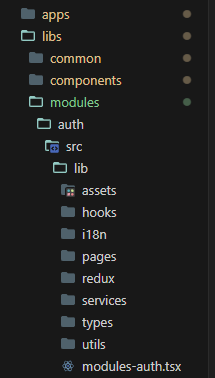
\includegraphics[width=0.3\textwidth]{graphics/sys-design/frontend_folder_structure_1.png}
  \caption{Frontend Source Code Structure}
  \label{fig:frontend_structure}
\end{figure} 


This structure allows us to develop each feature independently while maintaining code reusability and consistency throughout the project.

\subsection{Backend Source Code Structure}
The backend is developed using Java with Spring Boot, following a layered architecture pattern that promotes separation of concerns and maintainability. Our backend follows standard Java package naming conventions with a comprehensive structure organized by technical responsibility.

The main package structure reflects both cross-cutting concerns and feature modules:

\begin{itemize}
    \item \textbf{com.lcp} - Root package that contains all application code
    \begin{itemize}
        \item \textbf{base.dto} - Contains base data transfer object classes that establish inheritance hierarchies and common patterns for all DTOs in the system
        \item \textbf{common} - Houses utilities, constants, and common components shared across the entire application
        \item \textbf{configuration} - Contains Spring configuration classes, including bean definitions, property sources, and application profiles
        \item \textbf{exception} - Centralizes exception handling with custom exception classes and global exception handlers
        \item \textbf{security} - Implements authentication, authorization, and other security-related functionality
        \item \textbf{util} - Provides general-purpose utility classes that support various operations throughout the application
    \end{itemize}
\end{itemize}

Each business feature module follows a consistent layered architecture:

\begin{itemize}
    \item \textbf{/controller} - Contains REST API endpoints that handle HTTP requests and responses. Controllers are responsible for request validation, authentication verification, and routing to appropriate service methods.
    
    \item \textbf{/dto} - Data Transfer Objects that define the structure of data exchanged between the client and server. These objects isolate the internal entity model from external API contracts.
    
    \item \textbf{/entity} - JPA entity classes that map directly to database tables. These classes include field definitions, relationships, constraints, and JPA annotations.
    
    \item \textbf{/mapper} - Contains object mapper classes that transform data between entities and DTOs, ensuring clean separation between persistence and API layers.
    
    \item \textbf{/repository} - Implements the data access layer using Spring Data JPA repositories. These interfaces provide methods for CRUD operations and custom queries against the database.
    
    \item \textbf{/service} - Houses the business logic implementation. Service classes orchestrate operations across multiple repositories, implement transaction boundaries, and enforce business rules.
    
    \item \textbf{/common} - Module-specific utilities, constants, and shared components that are relevant only within the scope of the particular module.
\end{itemize}

This layered architecture provides several benefits:

\begin{itemize}
    \item Clear separation of concerns, making the codebase easier to understand and maintain
    \item Improved testability with well-defined boundaries between layers
    \item Consistent patterns across different modules that reduce cognitive load for developers
    \item Flexibility to modify implementation details in one layer without affecting others
    \item Enhanced security through proper encapsulation of business logic and data access
\end{itemize}

\begin{figure}[H]
  \centering
  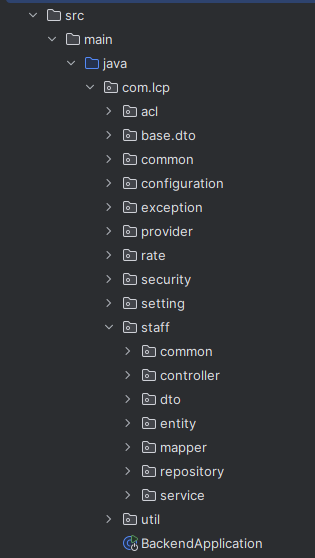
\includegraphics[width=0.3\textwidth]{graphics/sys-design/backend_folder_structure_2.png}
  \caption{Typical Module Internal Structure}
  \label{fig:module_structure}
\end{figure}

The architecture follows the dependency inversion principle, with controllers depending on services, which depend on repositories, creating a clean flow of control and data throughout the application.

\section{Interfaces implementation}
Below are the key interfaces implemented in our system, along with their respective functionalities:
% Authentication Interfaces
\begin{figure}[H]
    \centering
    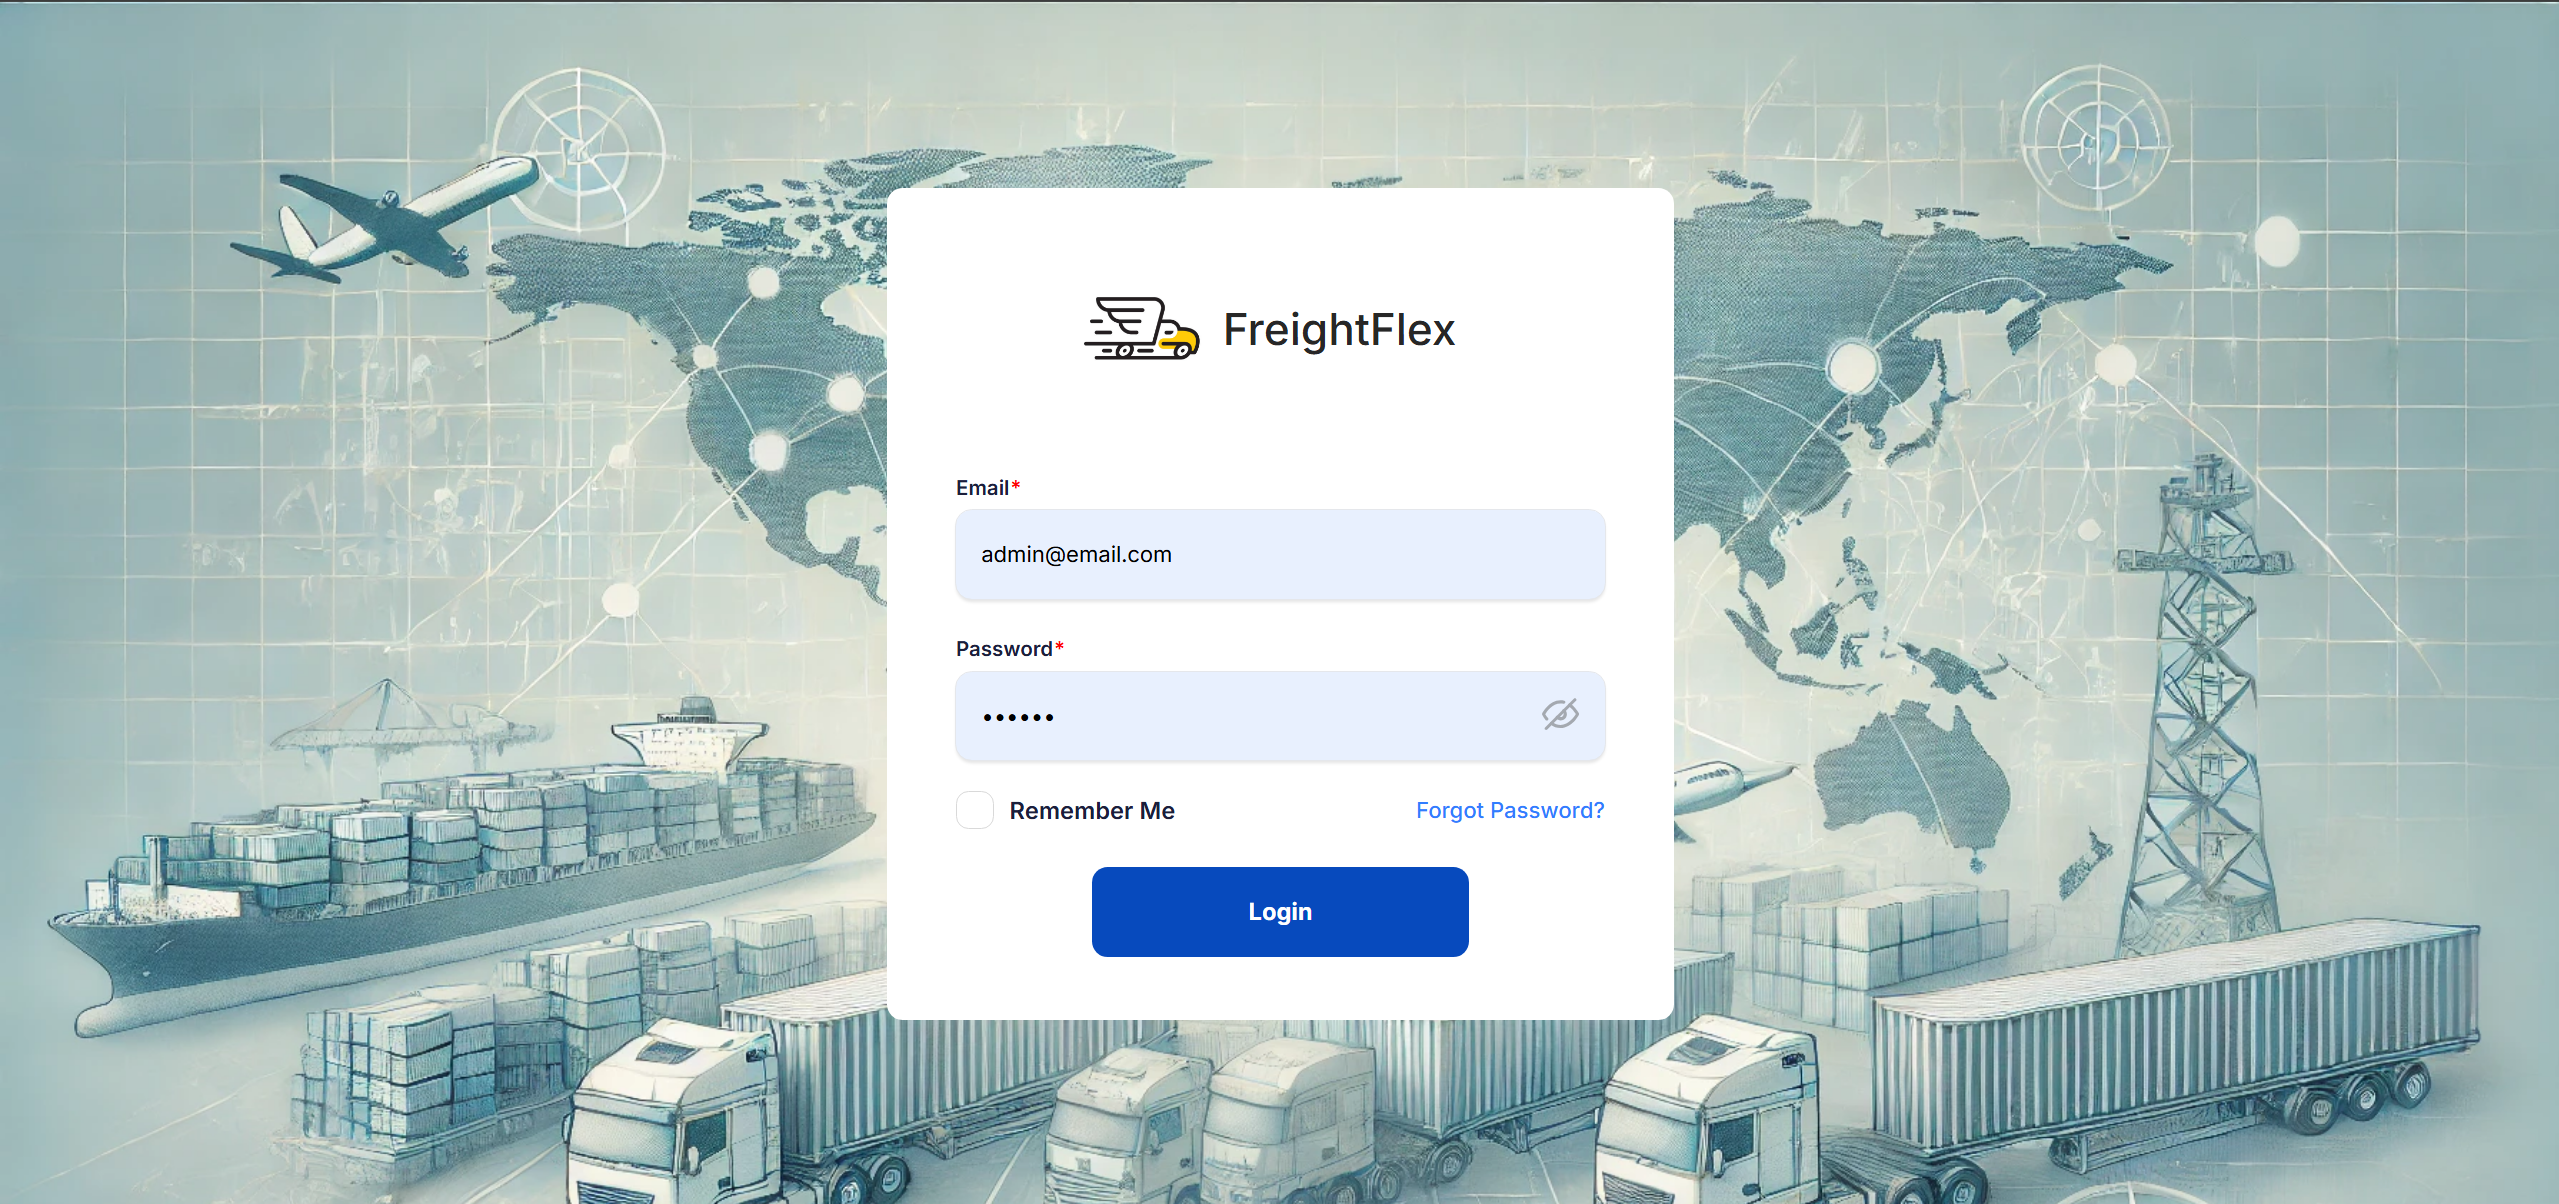
\includegraphics[width=15cm]{graphics/UI/login.png}
    \caption{Login Interface}
    \label{fig:login}
\end{figure}

\begin{figure}[H]
    \centering
    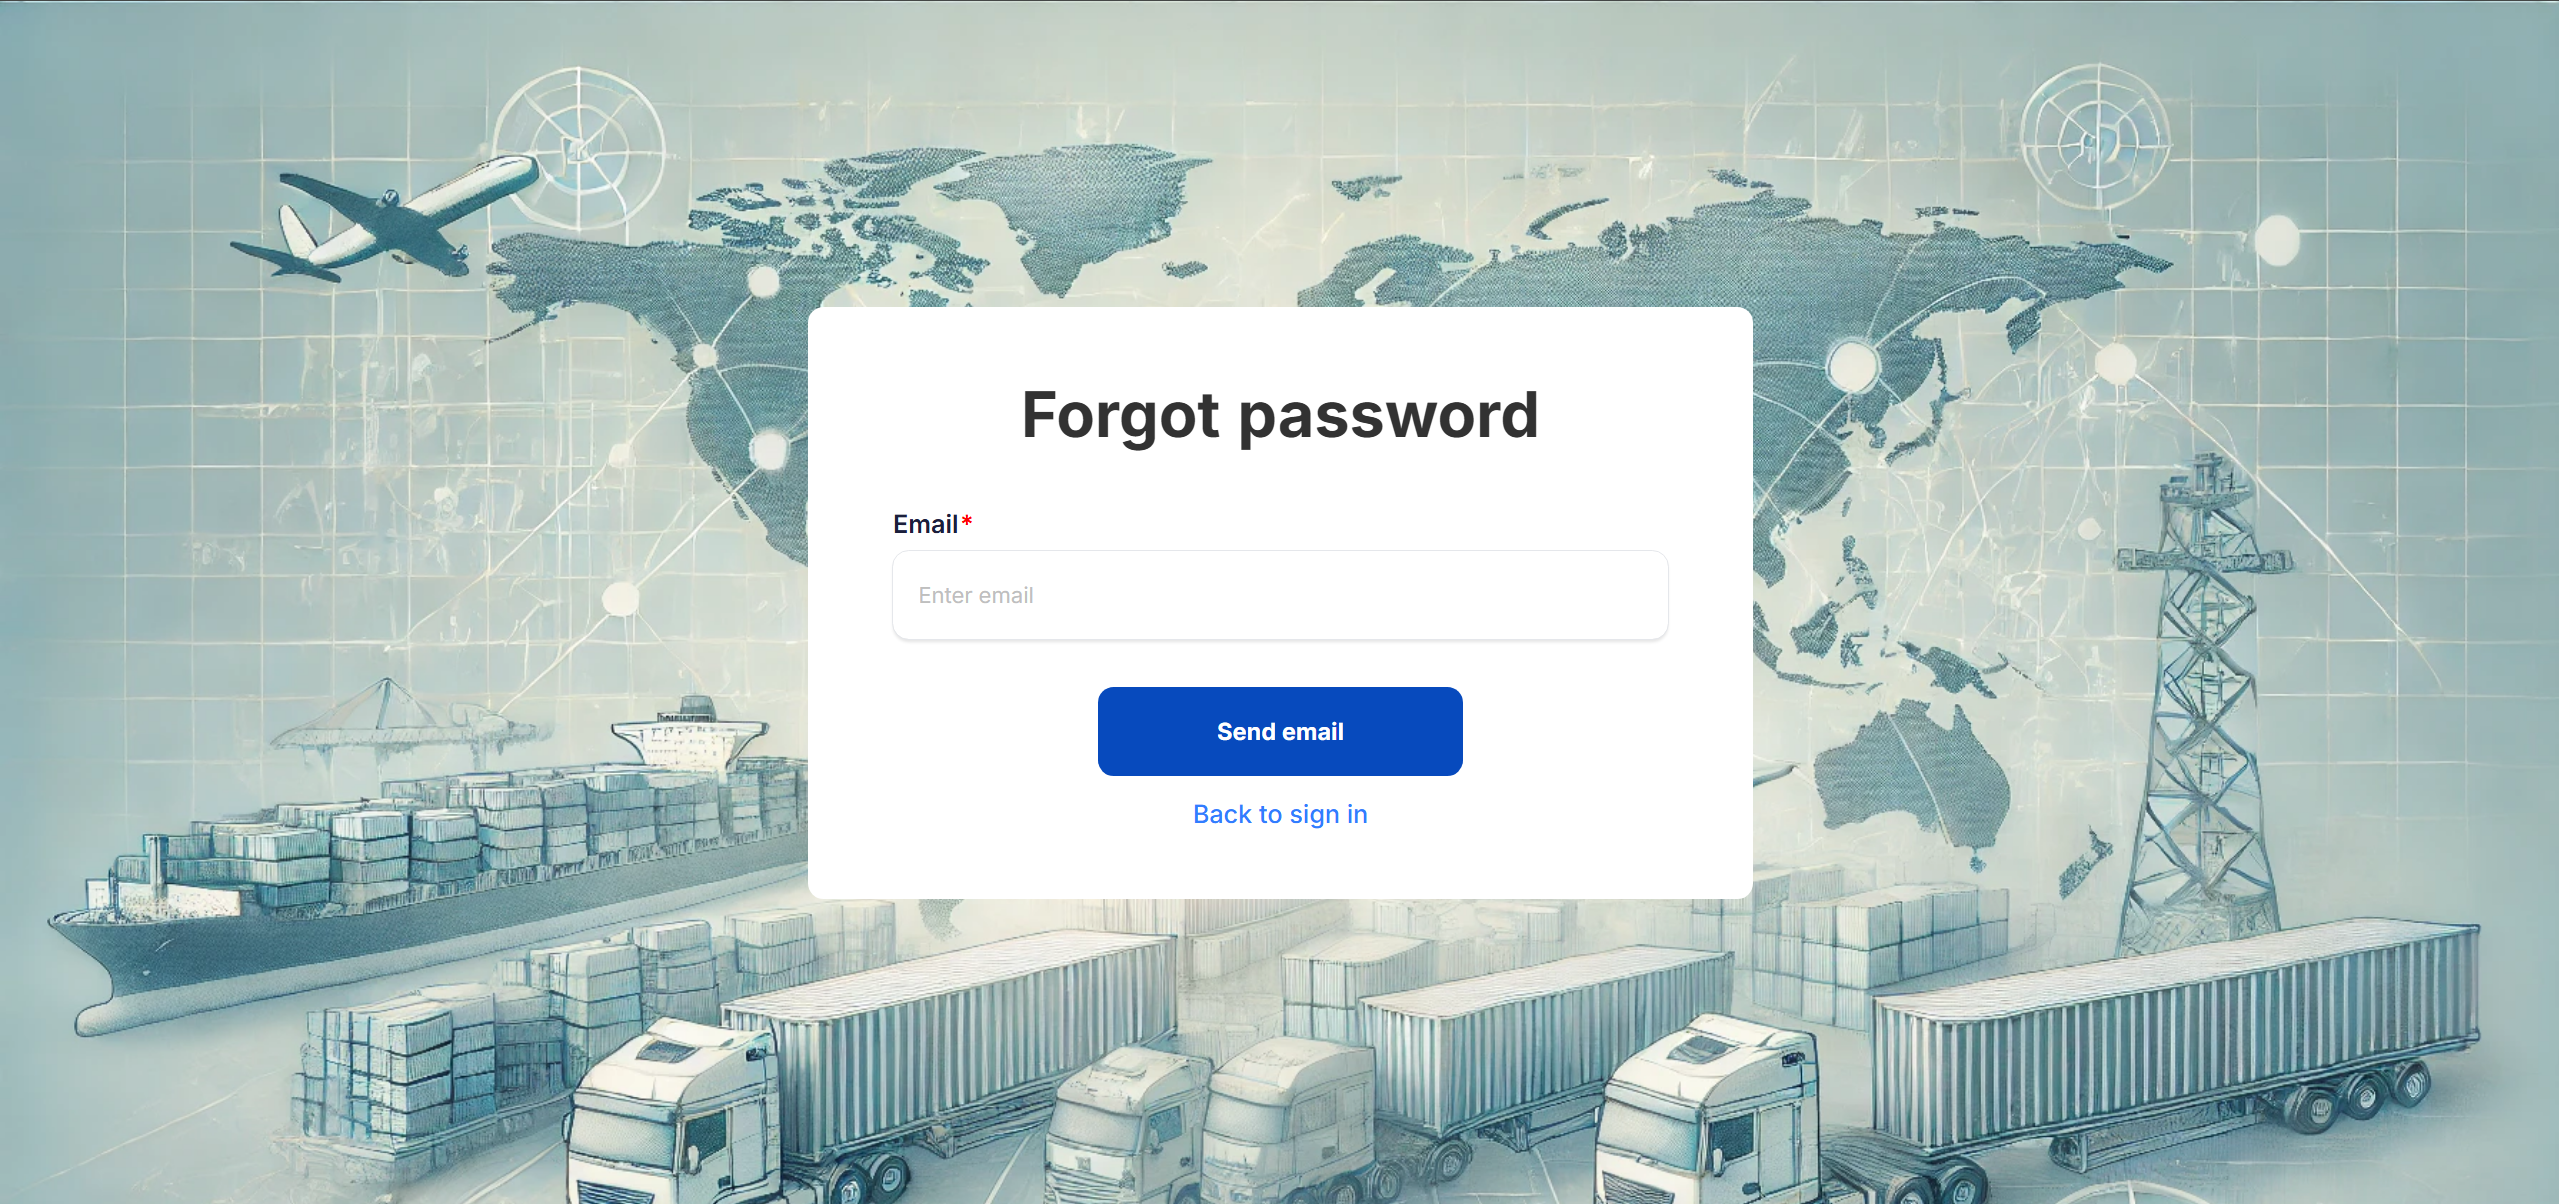
\includegraphics[width=15cm]{graphics/UI/forgot.png}
    \caption{Password Recovery Interface}
    \label{fig:forgot}
\end{figure}

% Main Dashboard Interface
\begin{figure}[H]
    \centering
    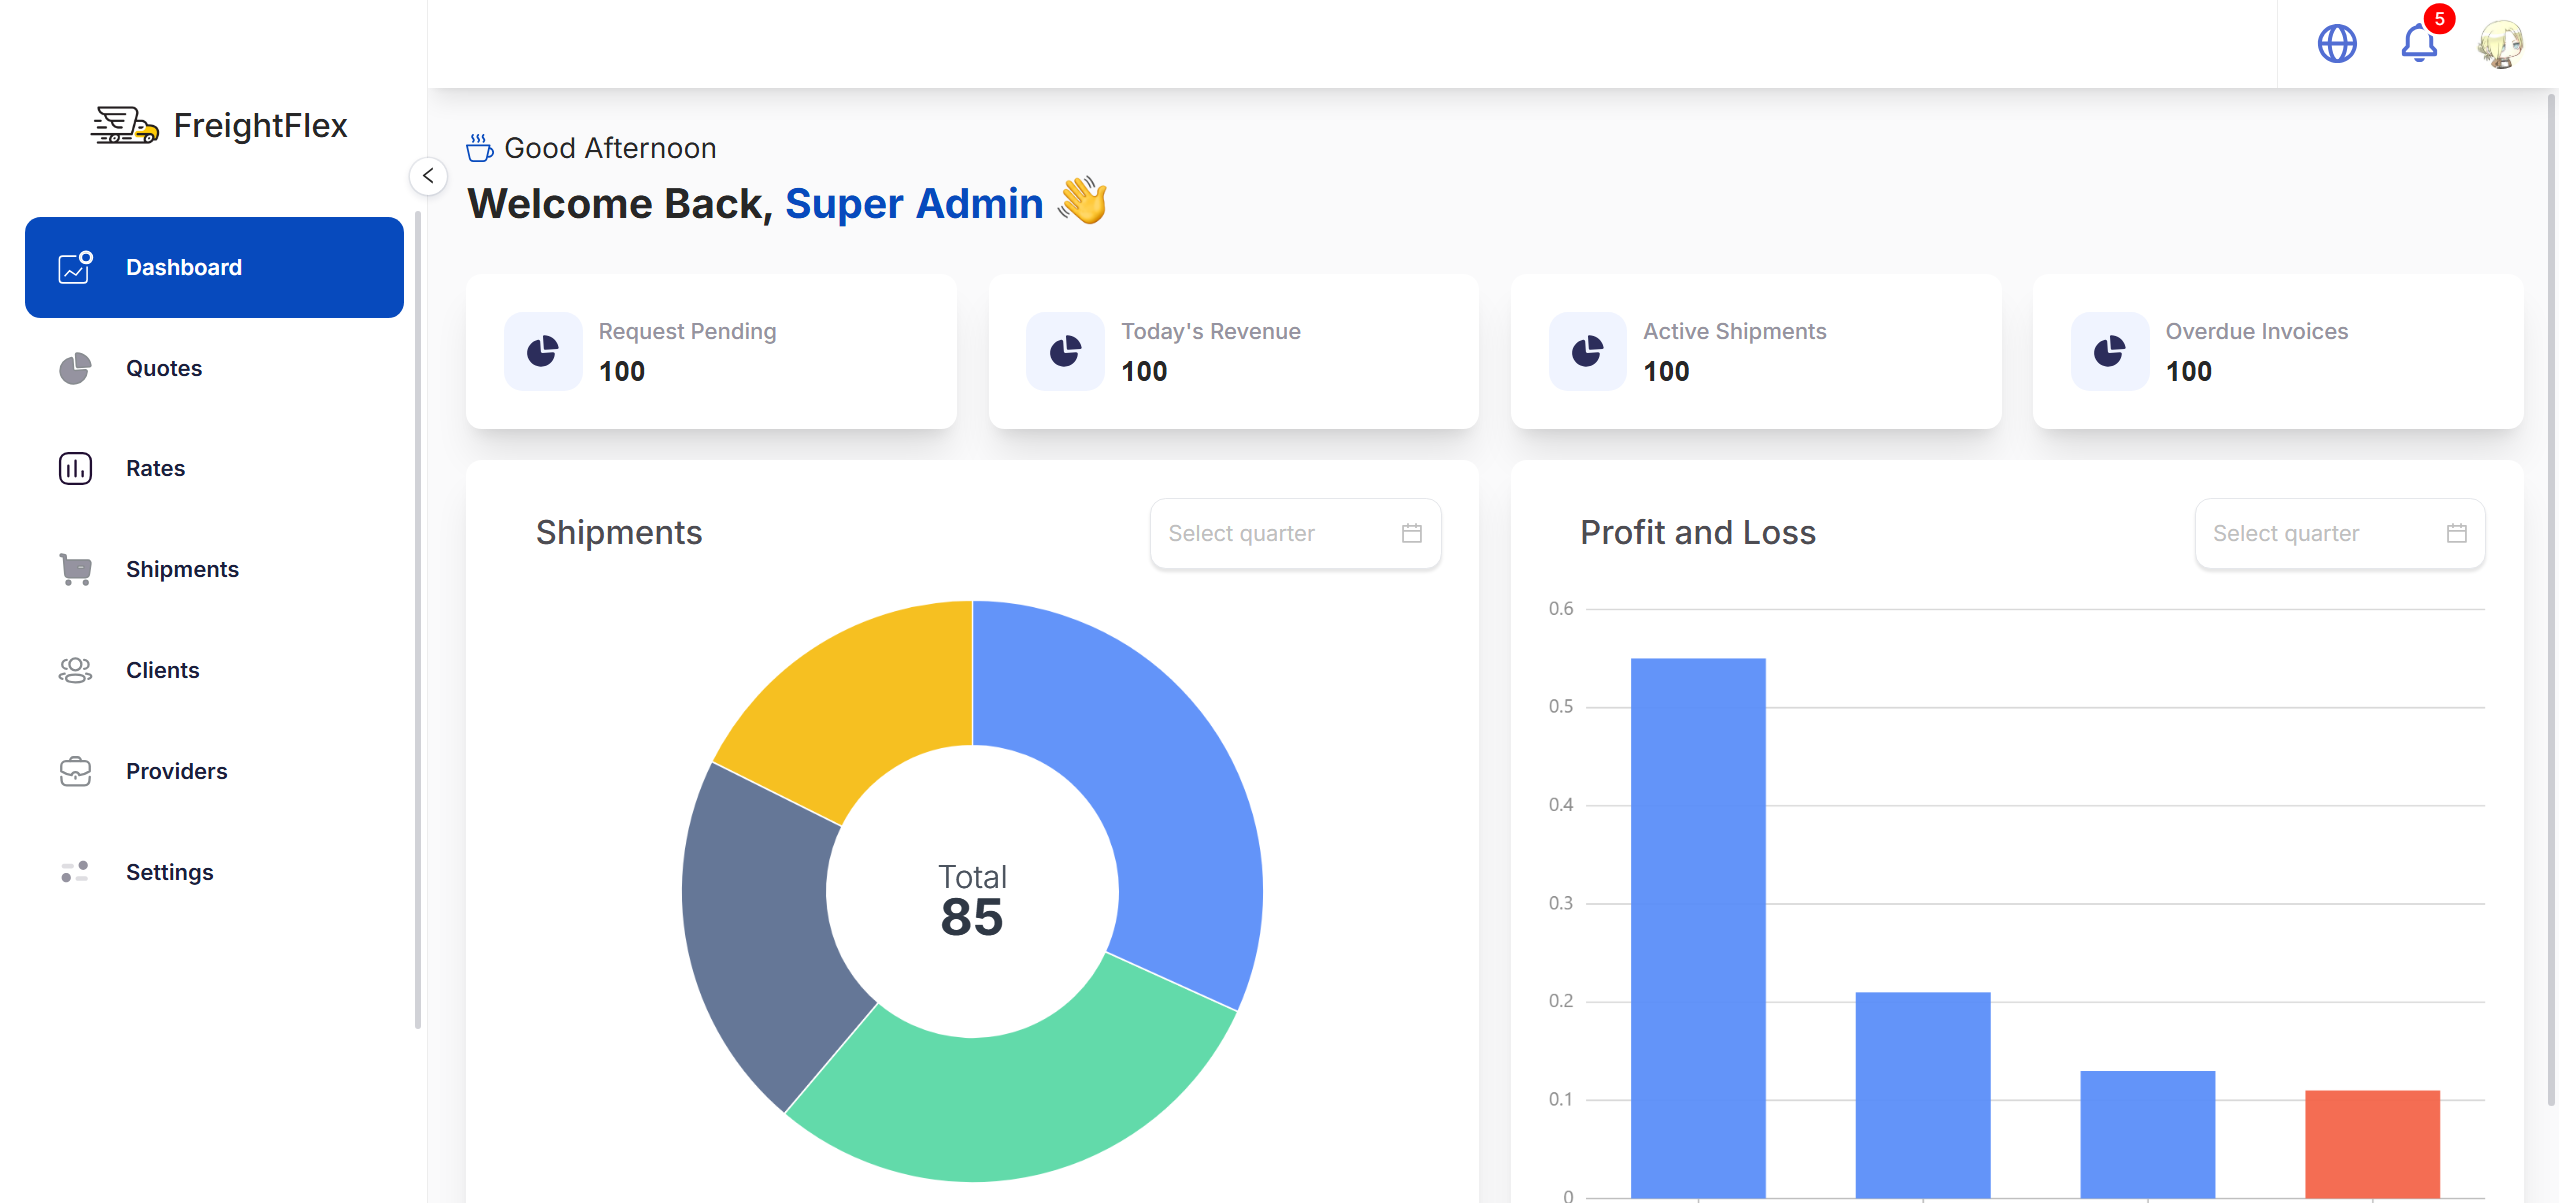
\includegraphics[width=15cm]{graphics/UI/admin-dashboard.png}
    \caption{Administrator Dashboard}
    \label{fig:admin-dashboard}
\end{figure}

% Landing Page
\begin{figure}[H]
    \centering
    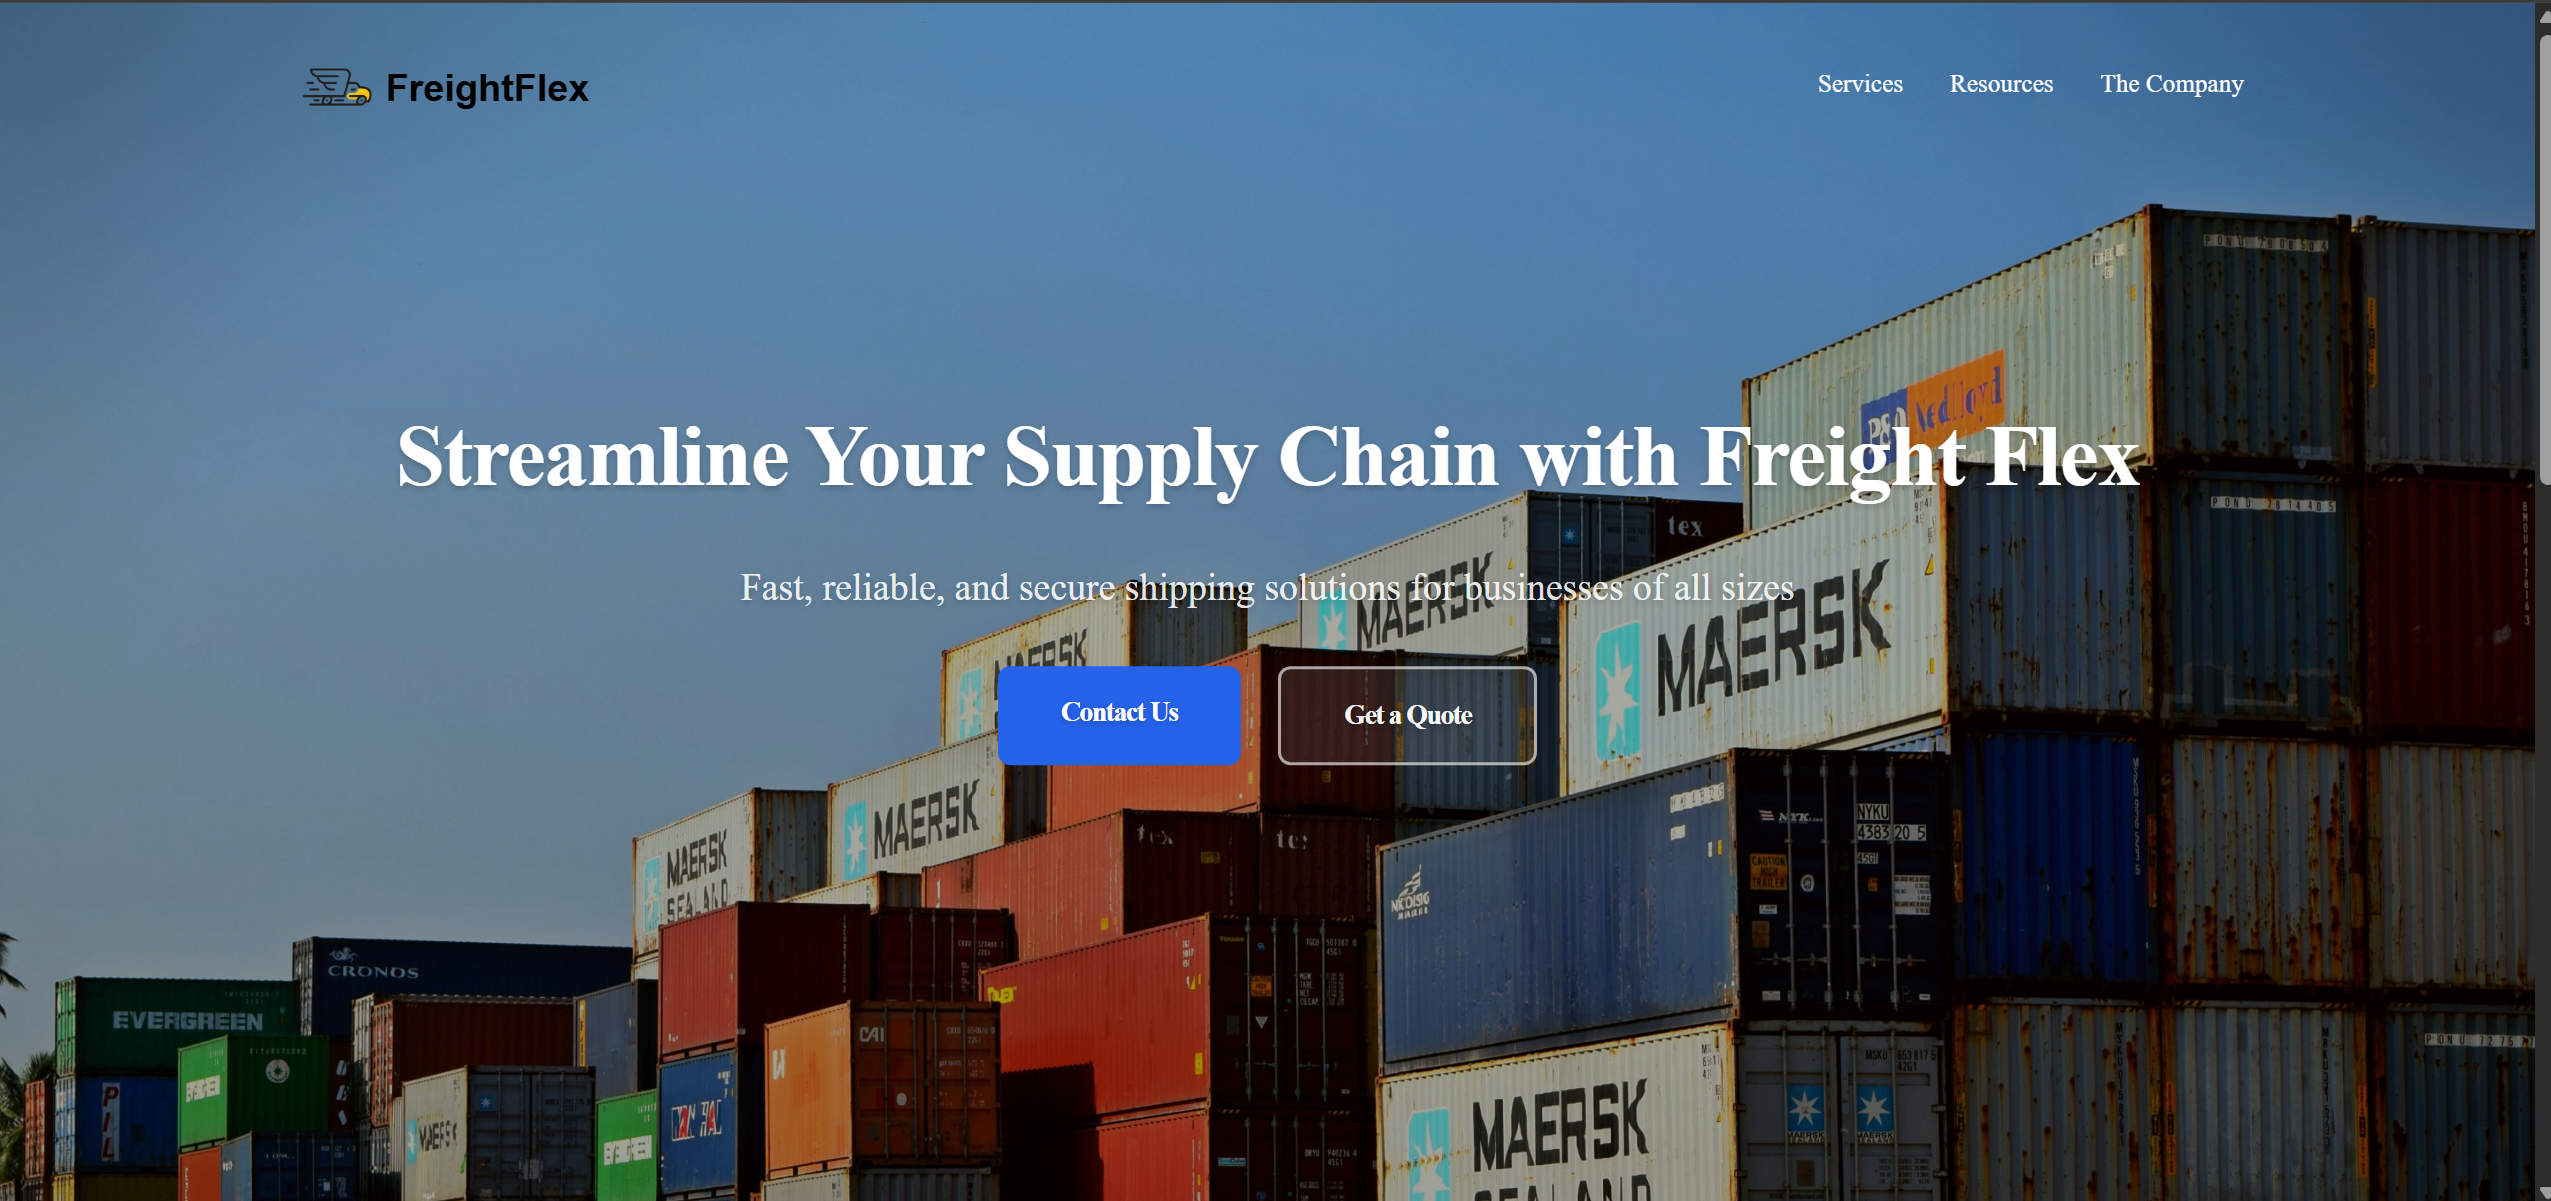
\includegraphics[width=15cm]{graphics/UI/landing-page.png}
    \caption{System Landing Page}
    \label{fig:landing-page}
\end{figure}

% Client Management Interfaces
\begin{figure}[H]
    \centering
    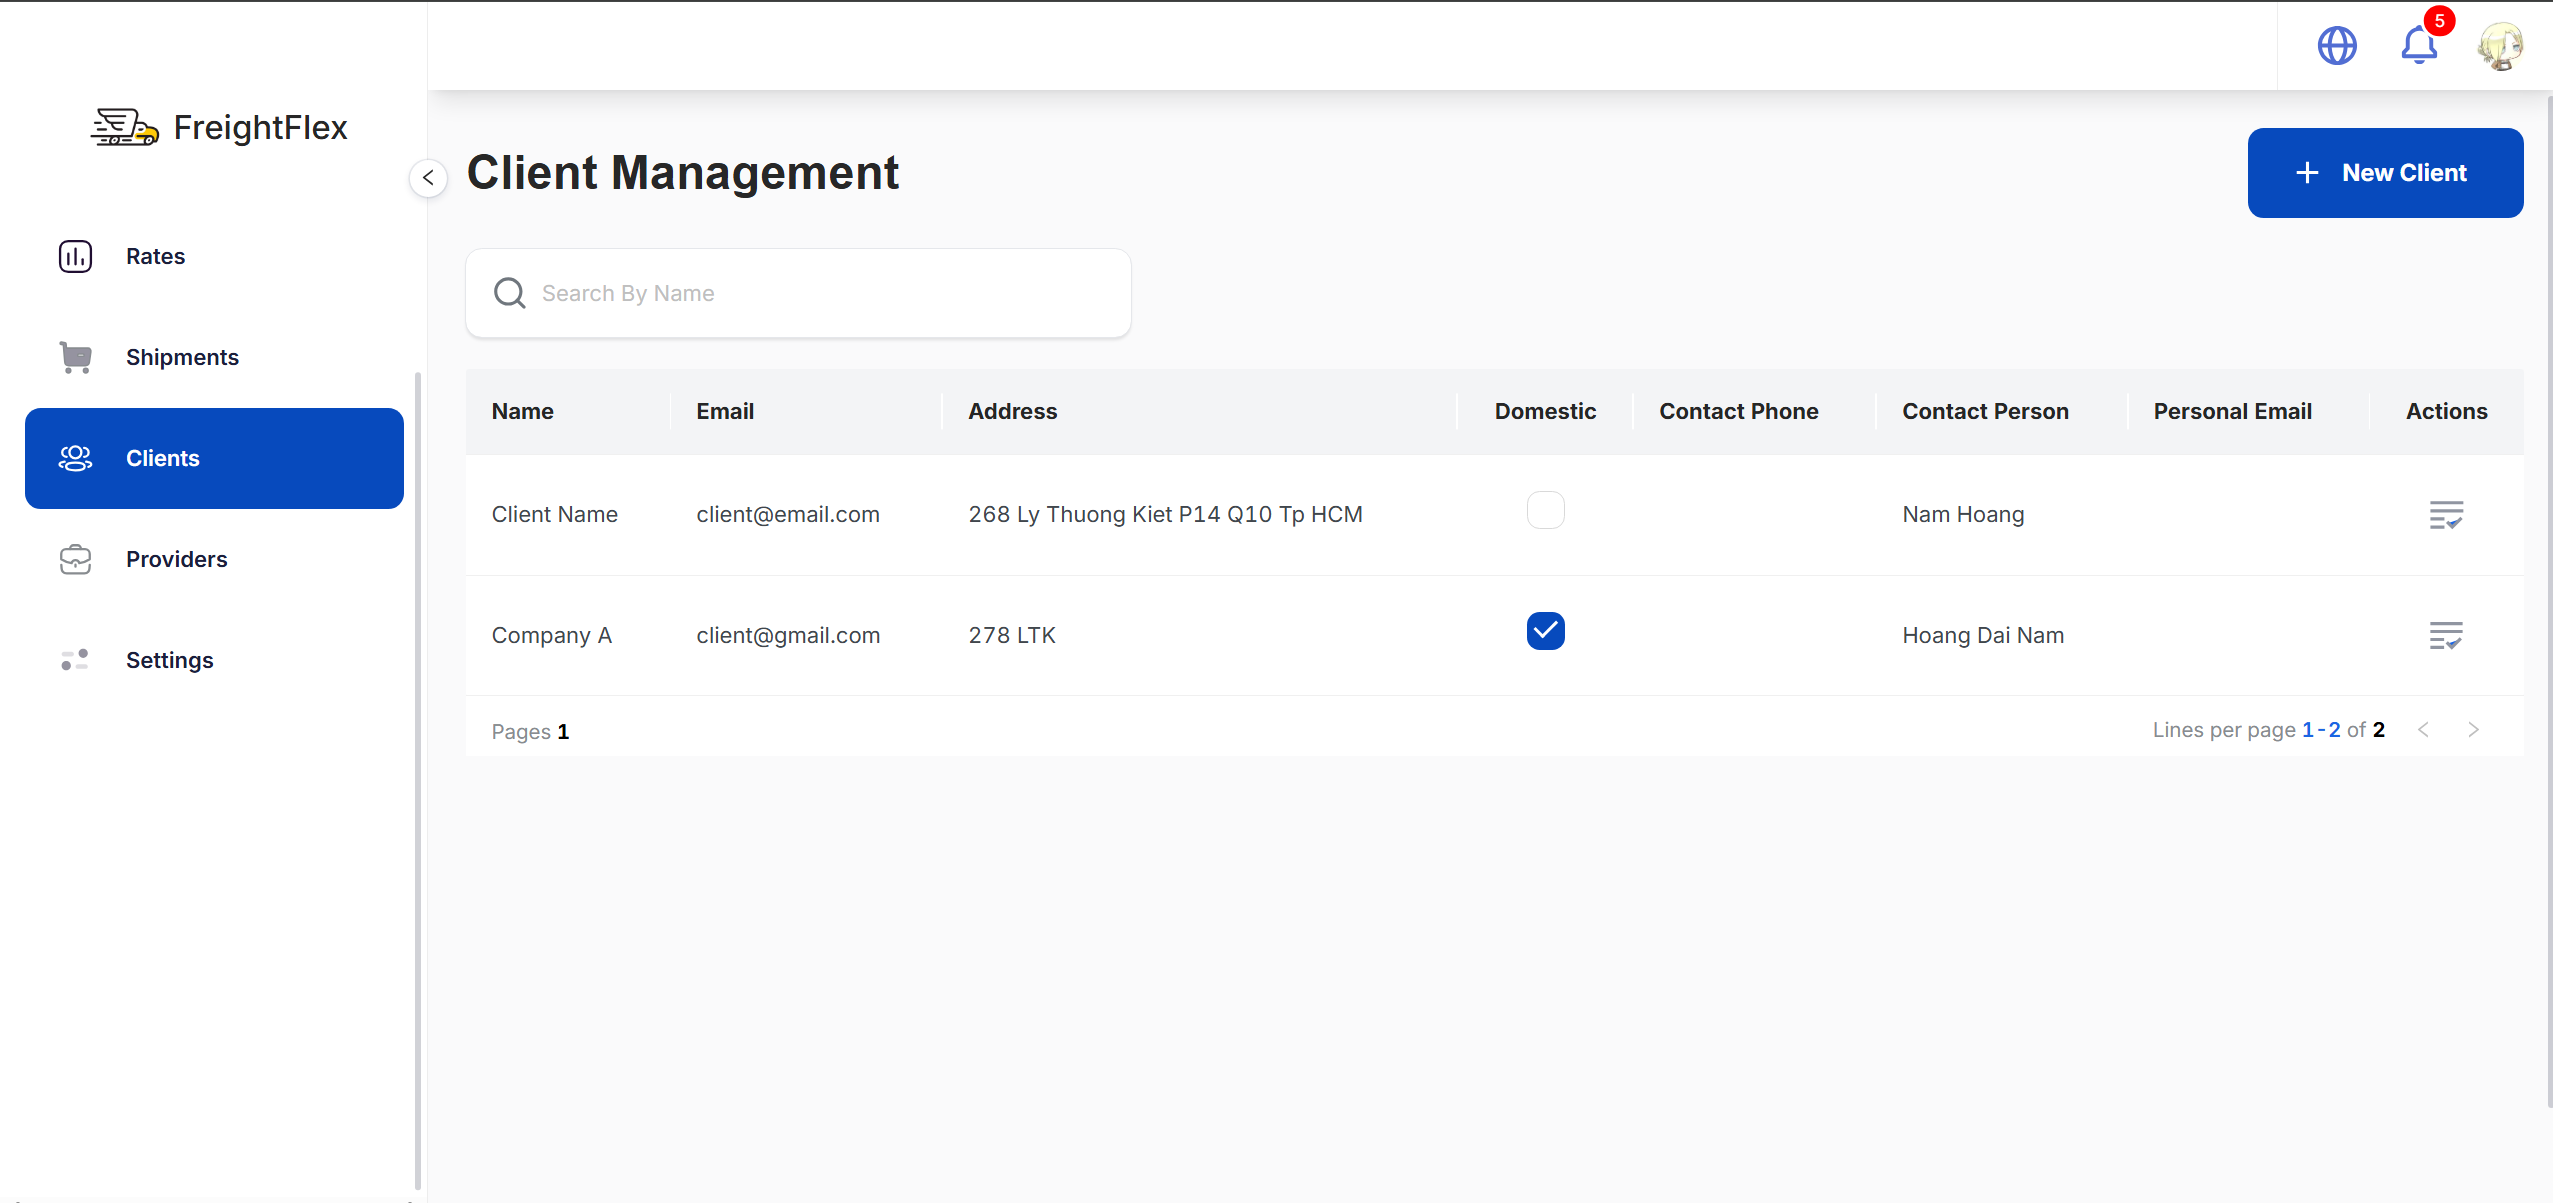
\includegraphics[width=15cm]{graphics/UI/client_management.png}
    \caption{Client Management Overview}
    \label{fig:client-management}
\end{figure}

\begin{figure}[H]
    \centering
    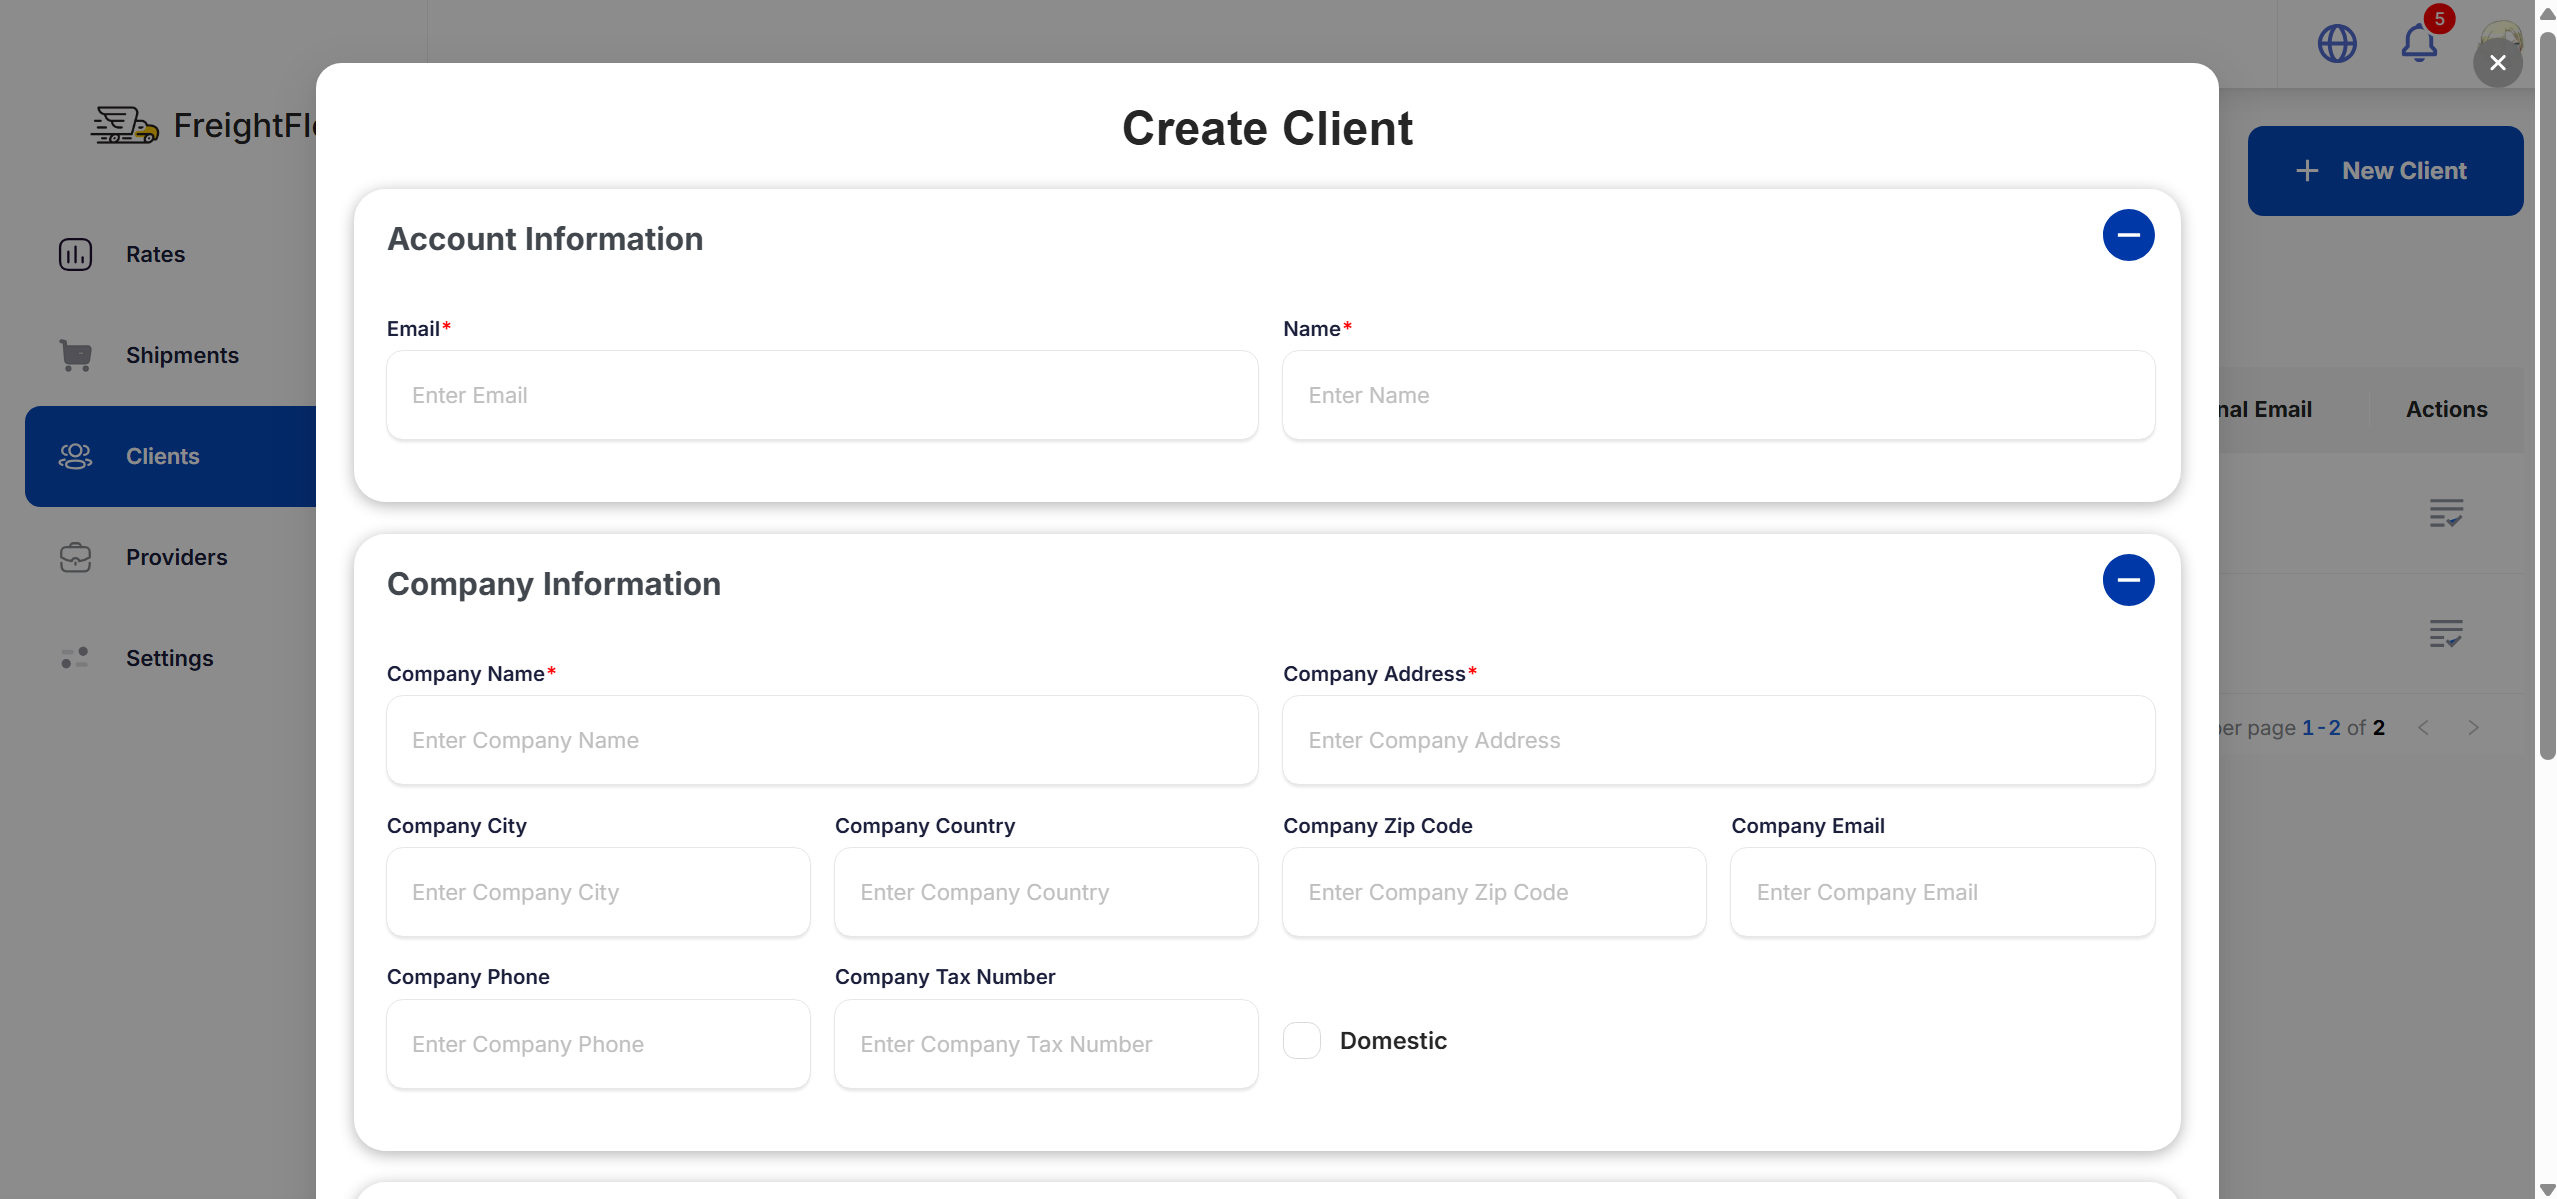
\includegraphics[width=15cm]{graphics/UI/new_client.png}
    \caption{New Client Registration}
    \label{fig:new-client}
\end{figure}

% User and Role Management
\begin{figure}[H]
    \centering
    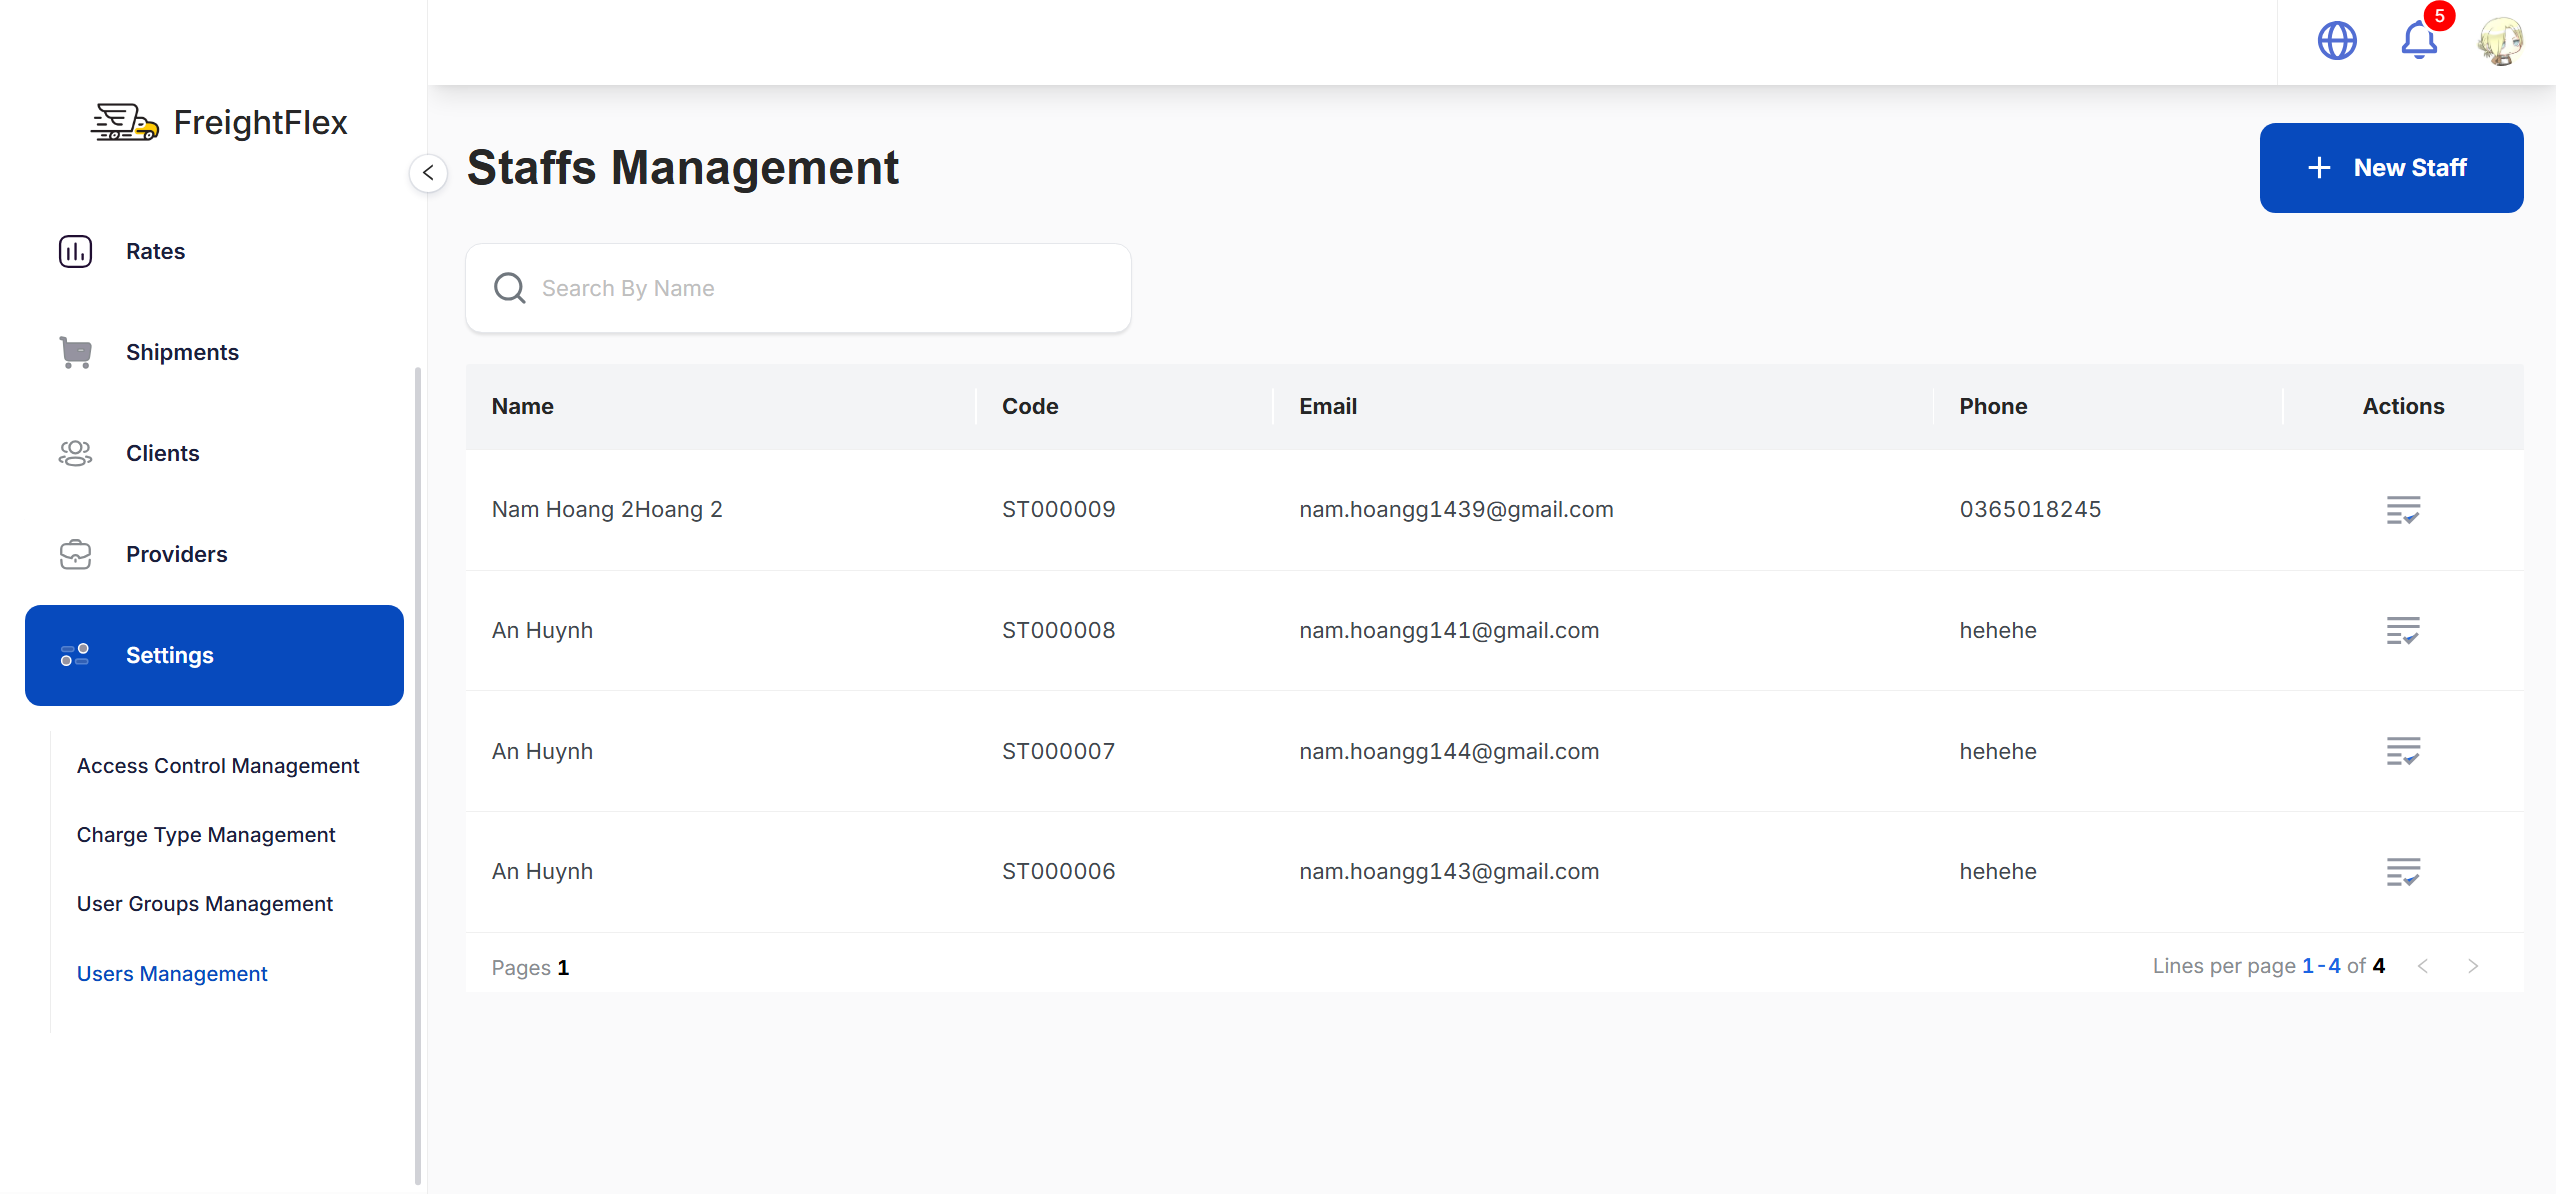
\includegraphics[width=15cm]{graphics/UI/user-management.png}
    \caption{User Management}
    \label{fig:user-management}
\end{figure}

\begin{figure}[H]
    \centering
    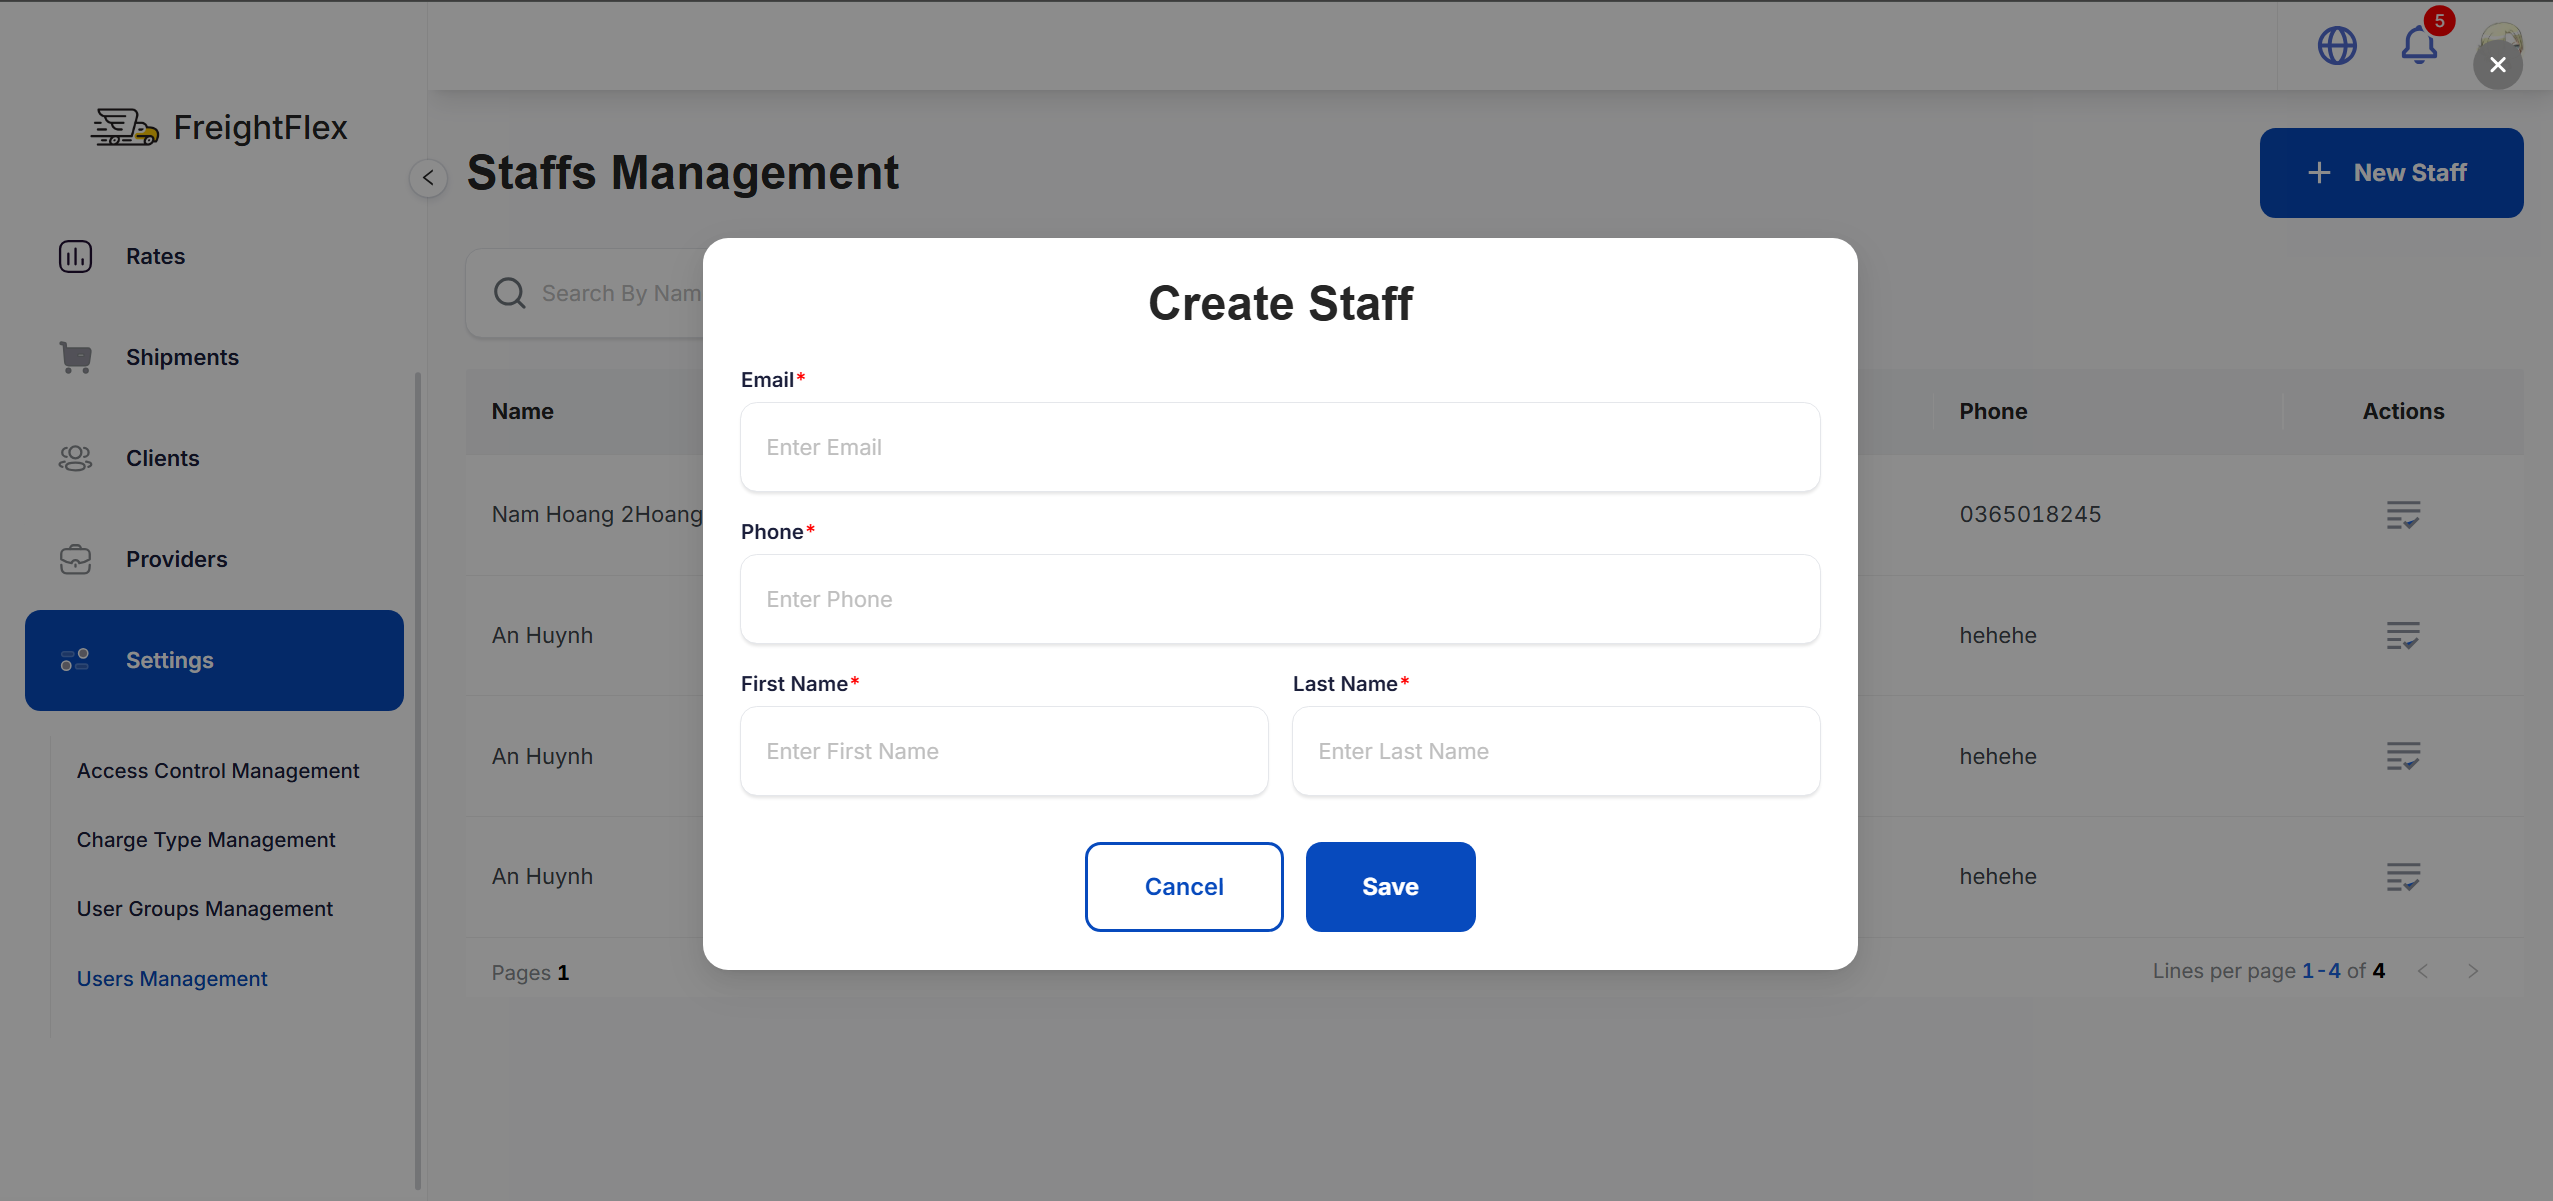
\includegraphics[width=15cm]{graphics/UI/new-user.png}
    \caption{New User Creation}
    \label{fig:new-user}
\end{figure}

\begin{figure}[H]
    \centering
    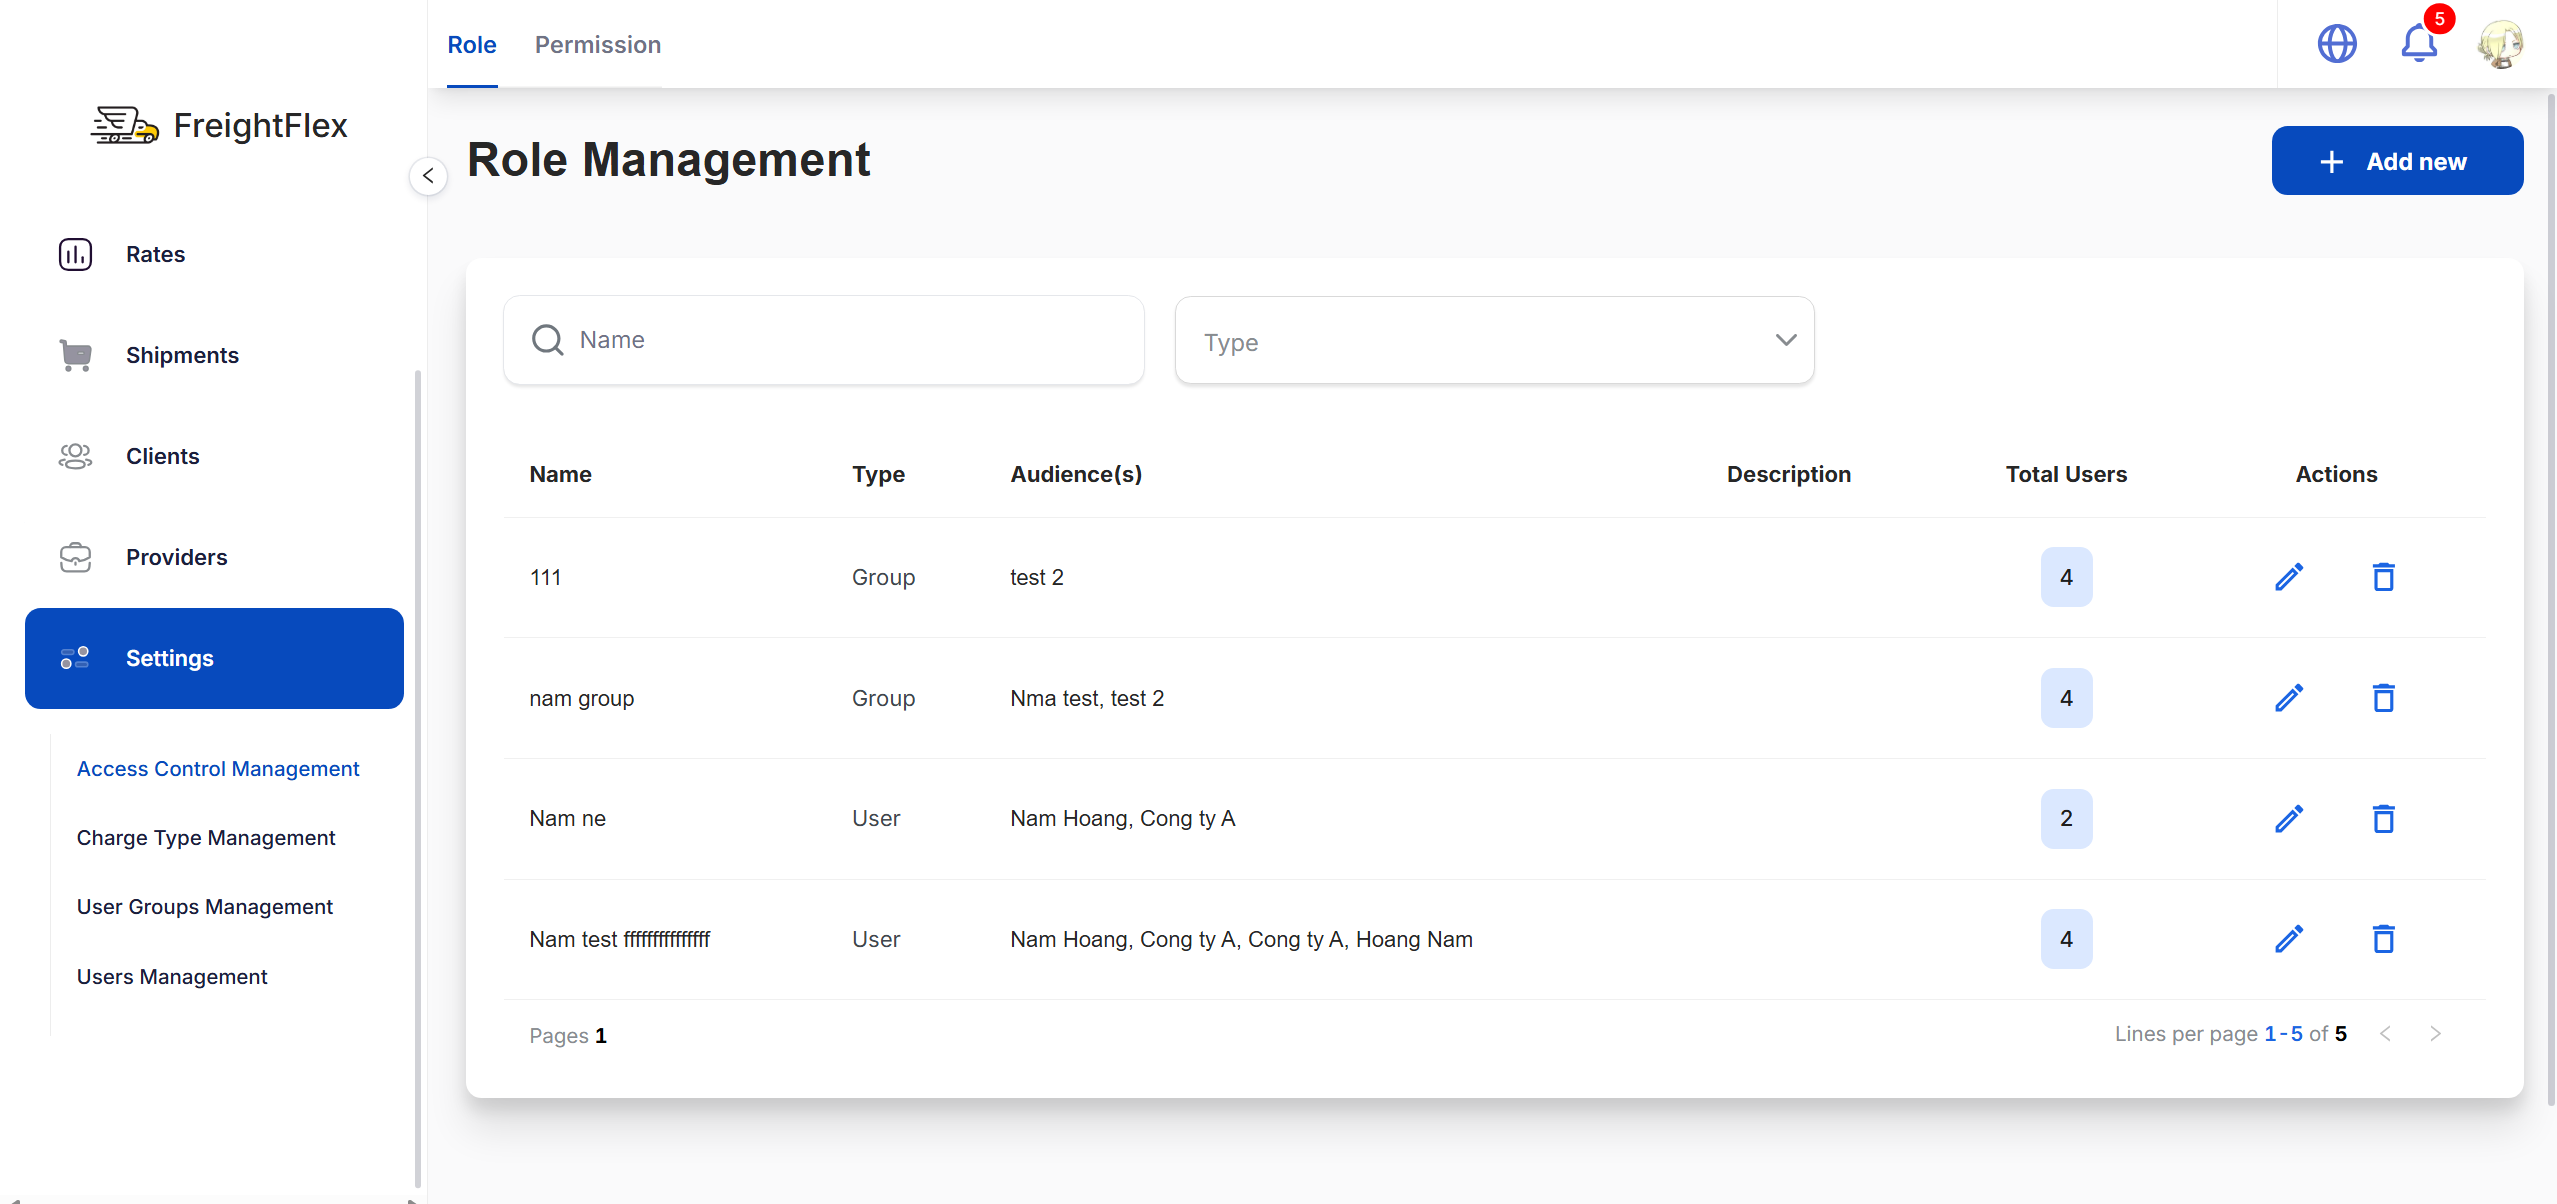
\includegraphics[width=15cm]{graphics/UI/role-management.png}
    \caption{Role Management}
    \label{fig:role-management}
\end{figure}

\begin{figure}[H]
    \centering
    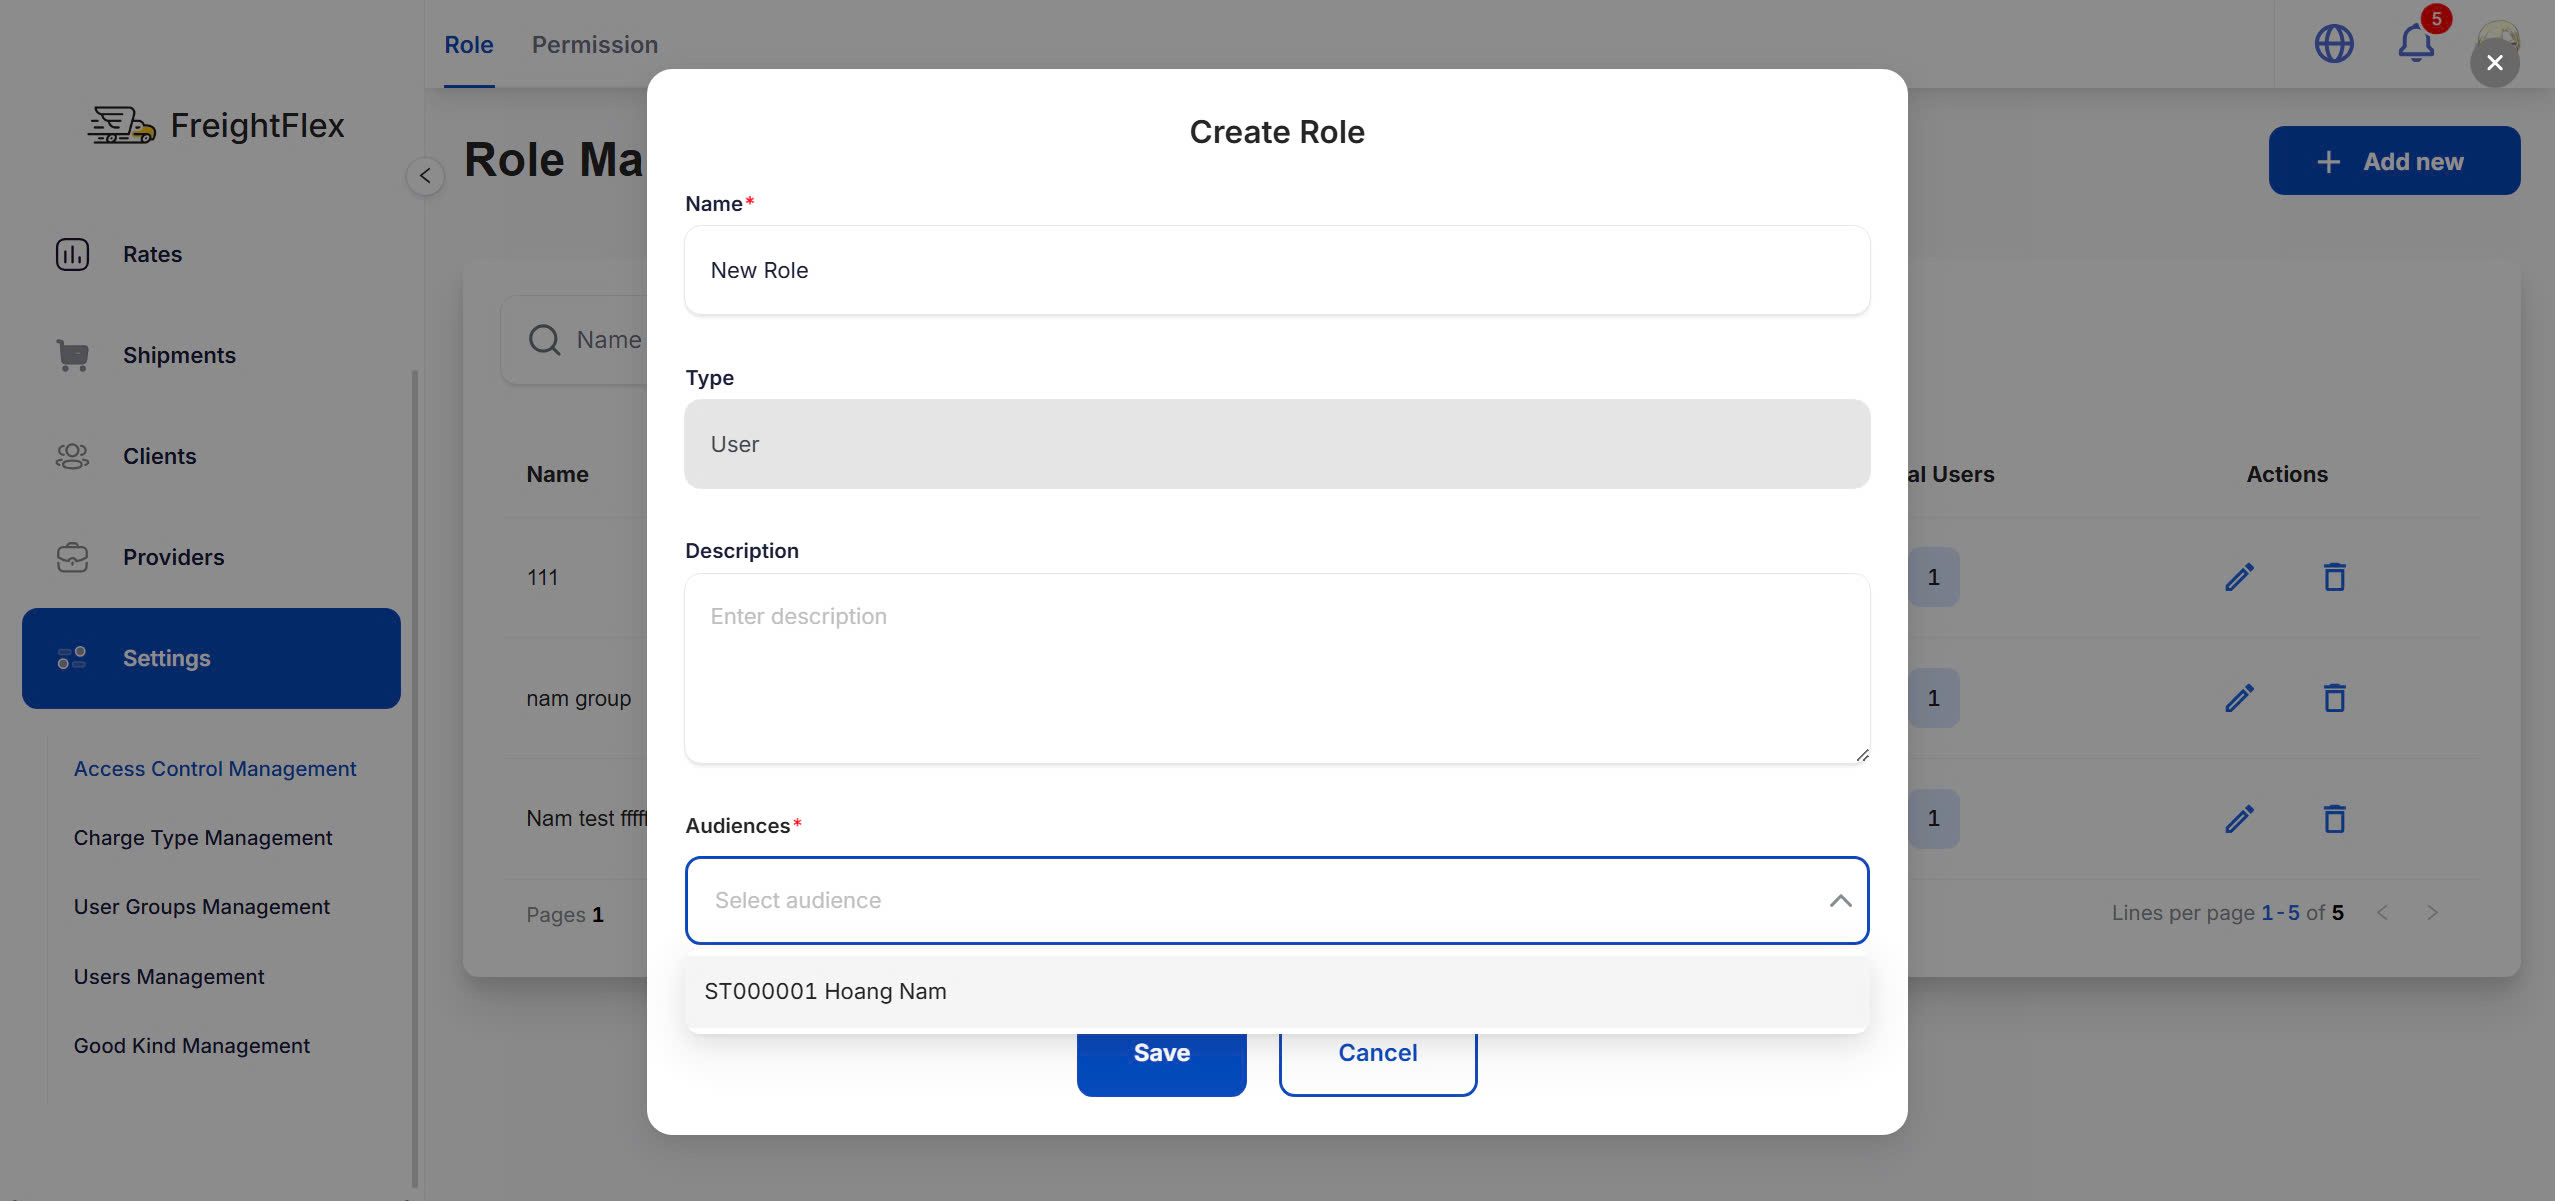
\includegraphics[width=15cm]{graphics/UI/new-role.png}
    \caption{New Role Creation}
    \label{fig:new-role}
\end{figure}

\begin{figure}[H]
    \centering
    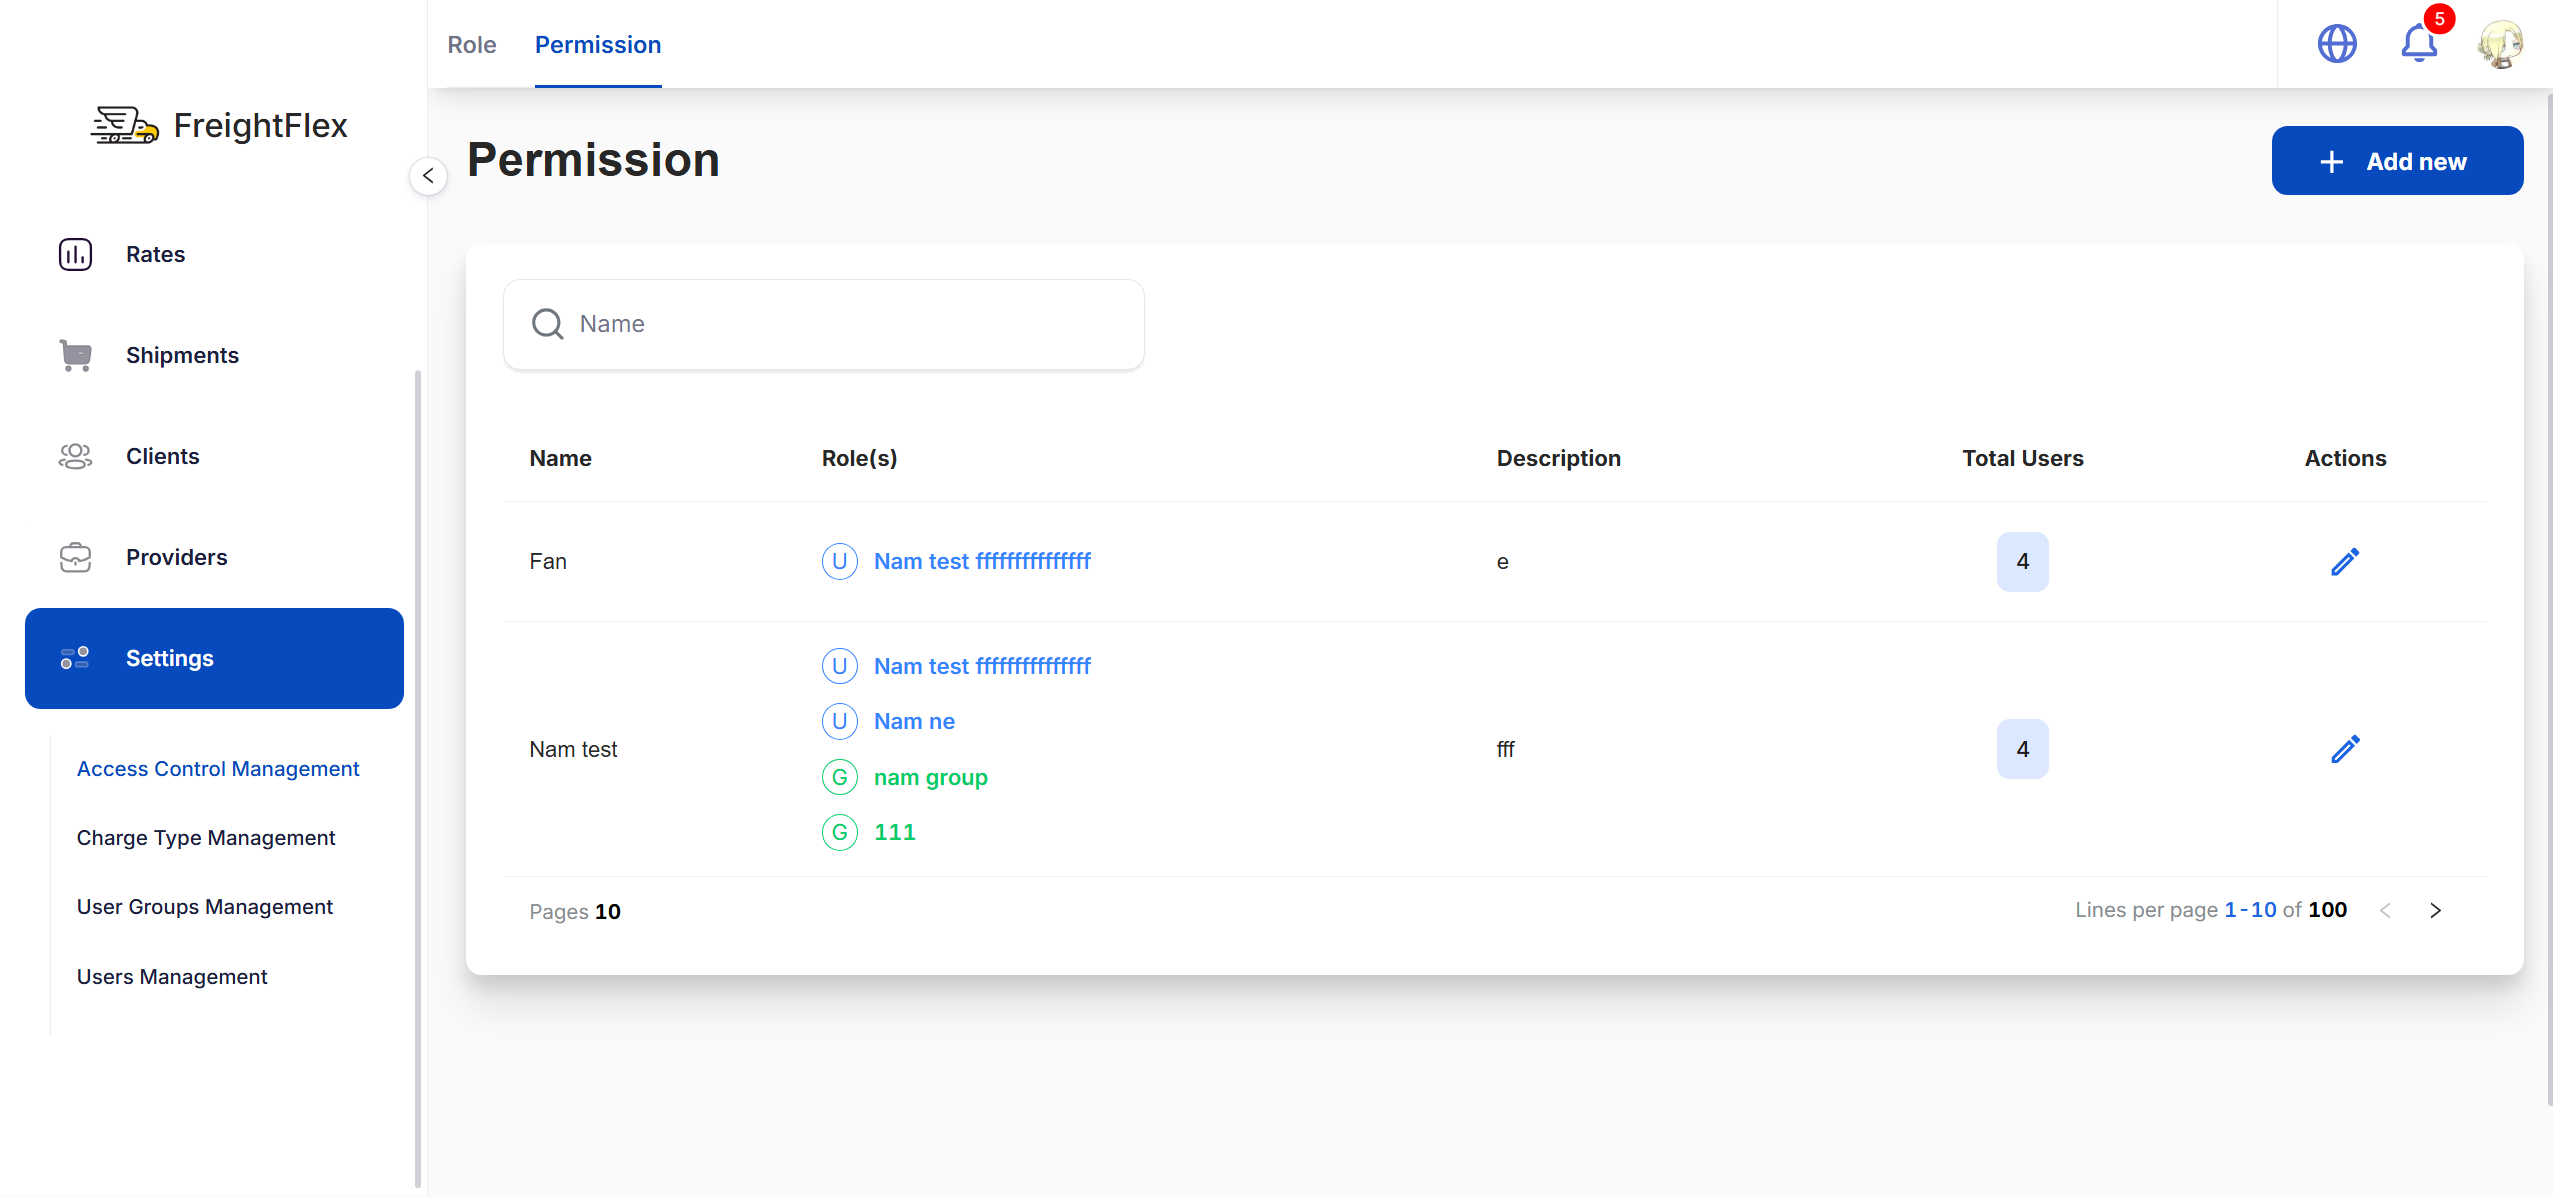
\includegraphics[width=15cm]{graphics/UI/permission-management.png}
    \caption{Permission Management}
    \label{fig:permission-management}
\end{figure}

\begin{figure}[H]
    \centering
    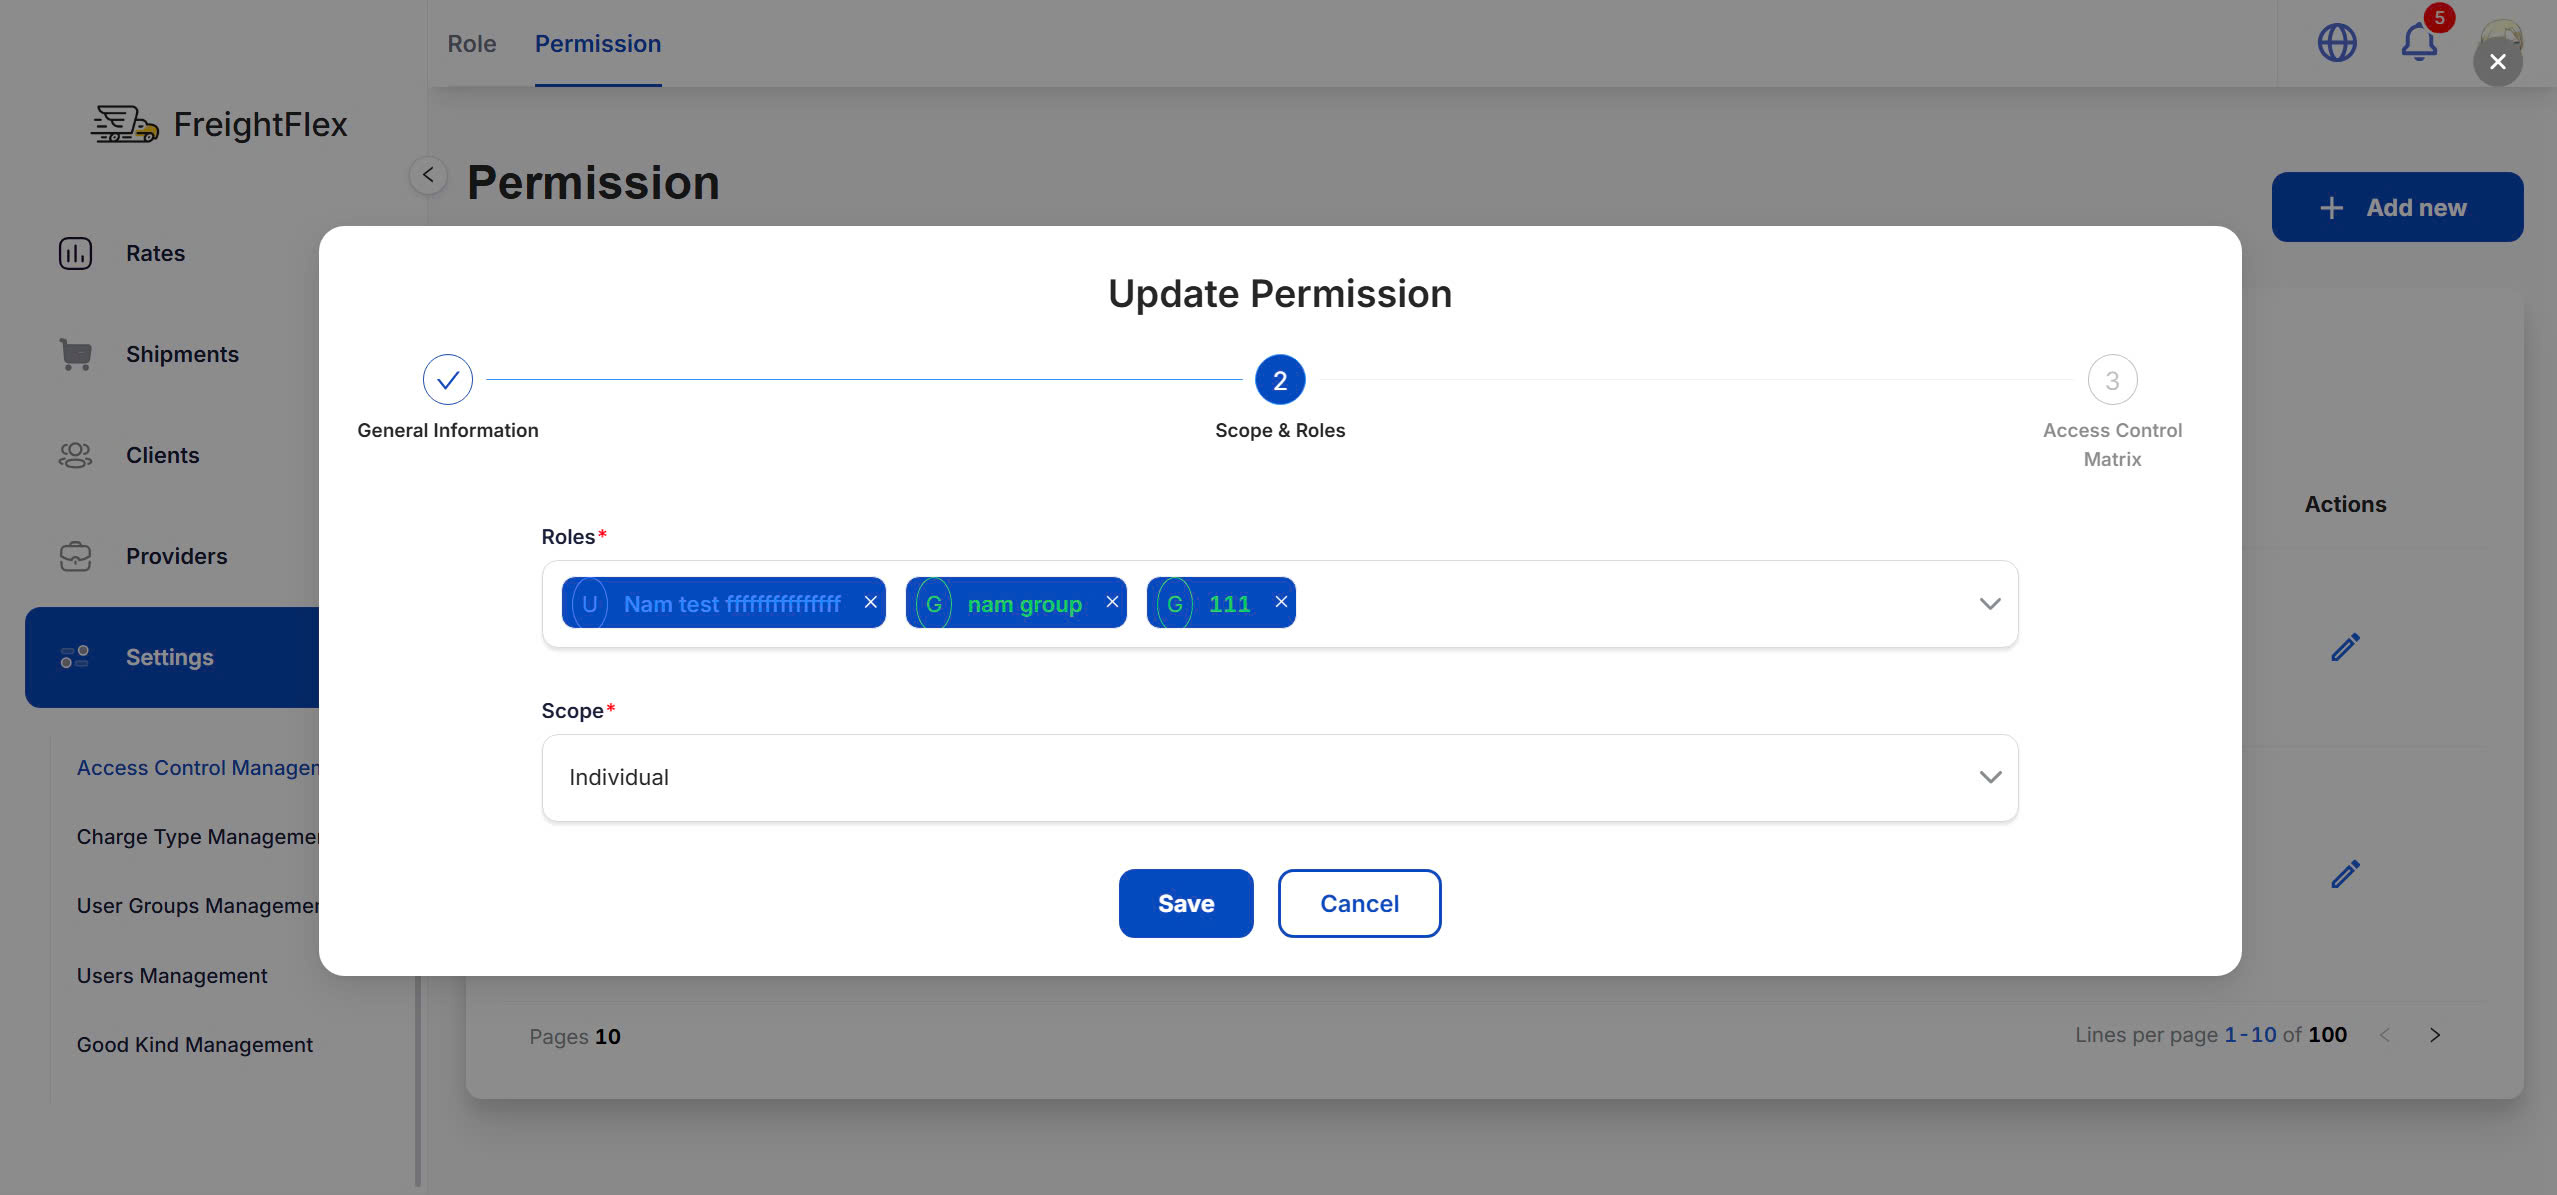
\includegraphics[width=15cm]{graphics/UI/new-permission.png}
    \caption{New Permission Creation}
    \label{fig:new-permission}
\end{figure}

\begin{figure}[H]
    \centering
    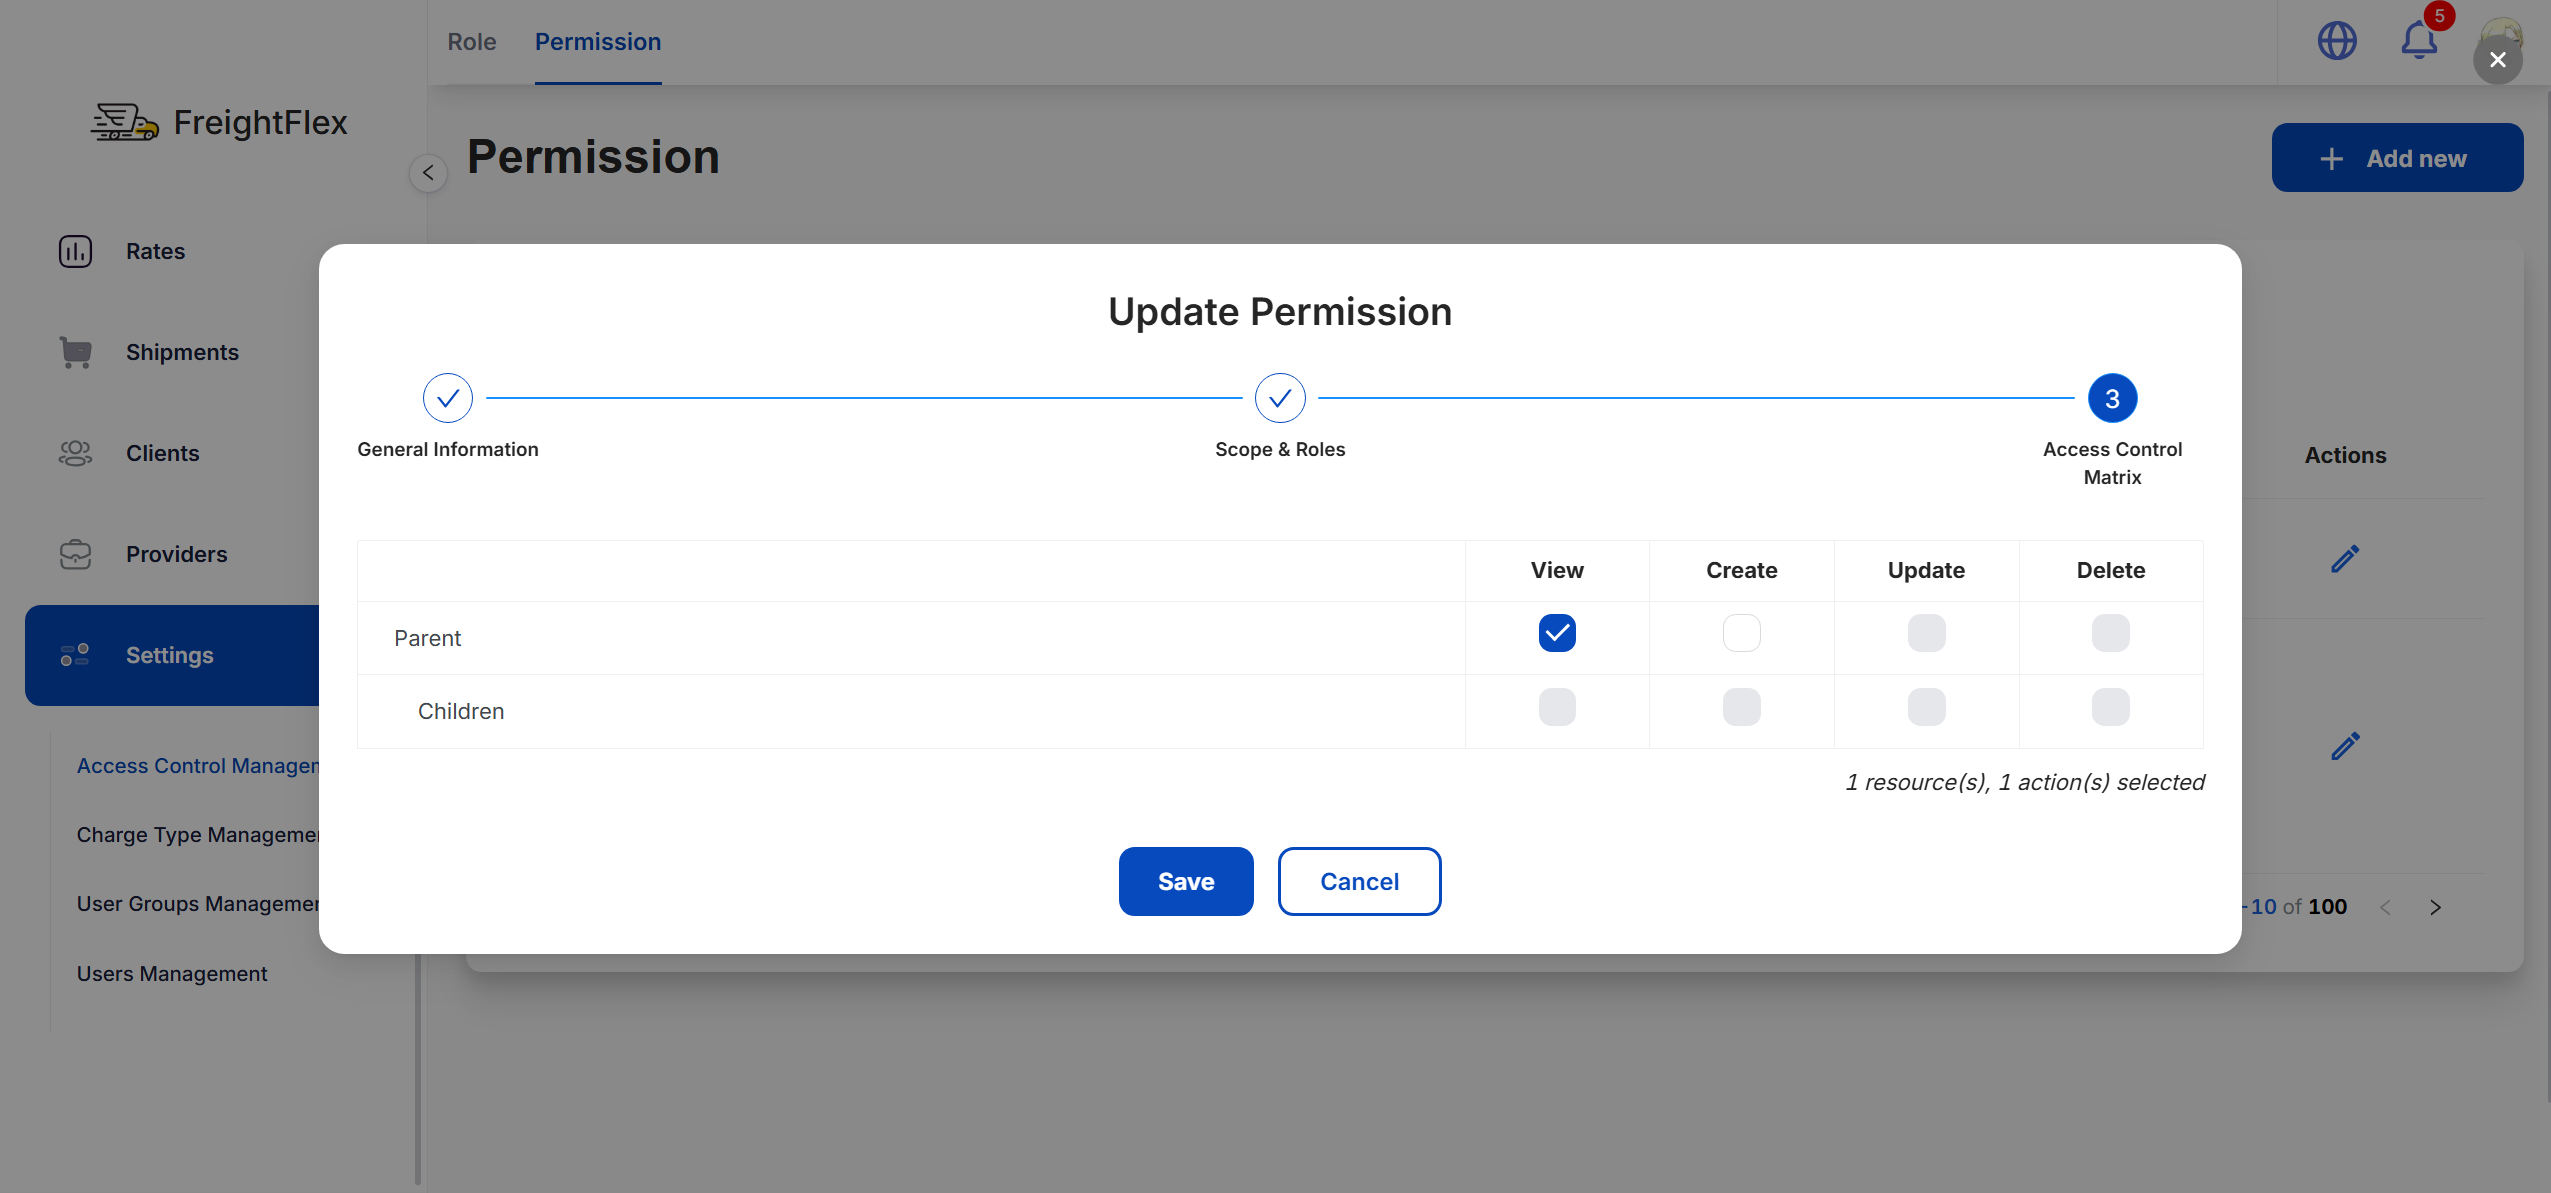
\includegraphics[width=15cm]{graphics/UI/new-permission-2.png}
    \caption{New Permission Creation}
    \label{fig:new-permission-2}
\end{figure}

% Group Management
\begin{figure}[H]
    \centering
    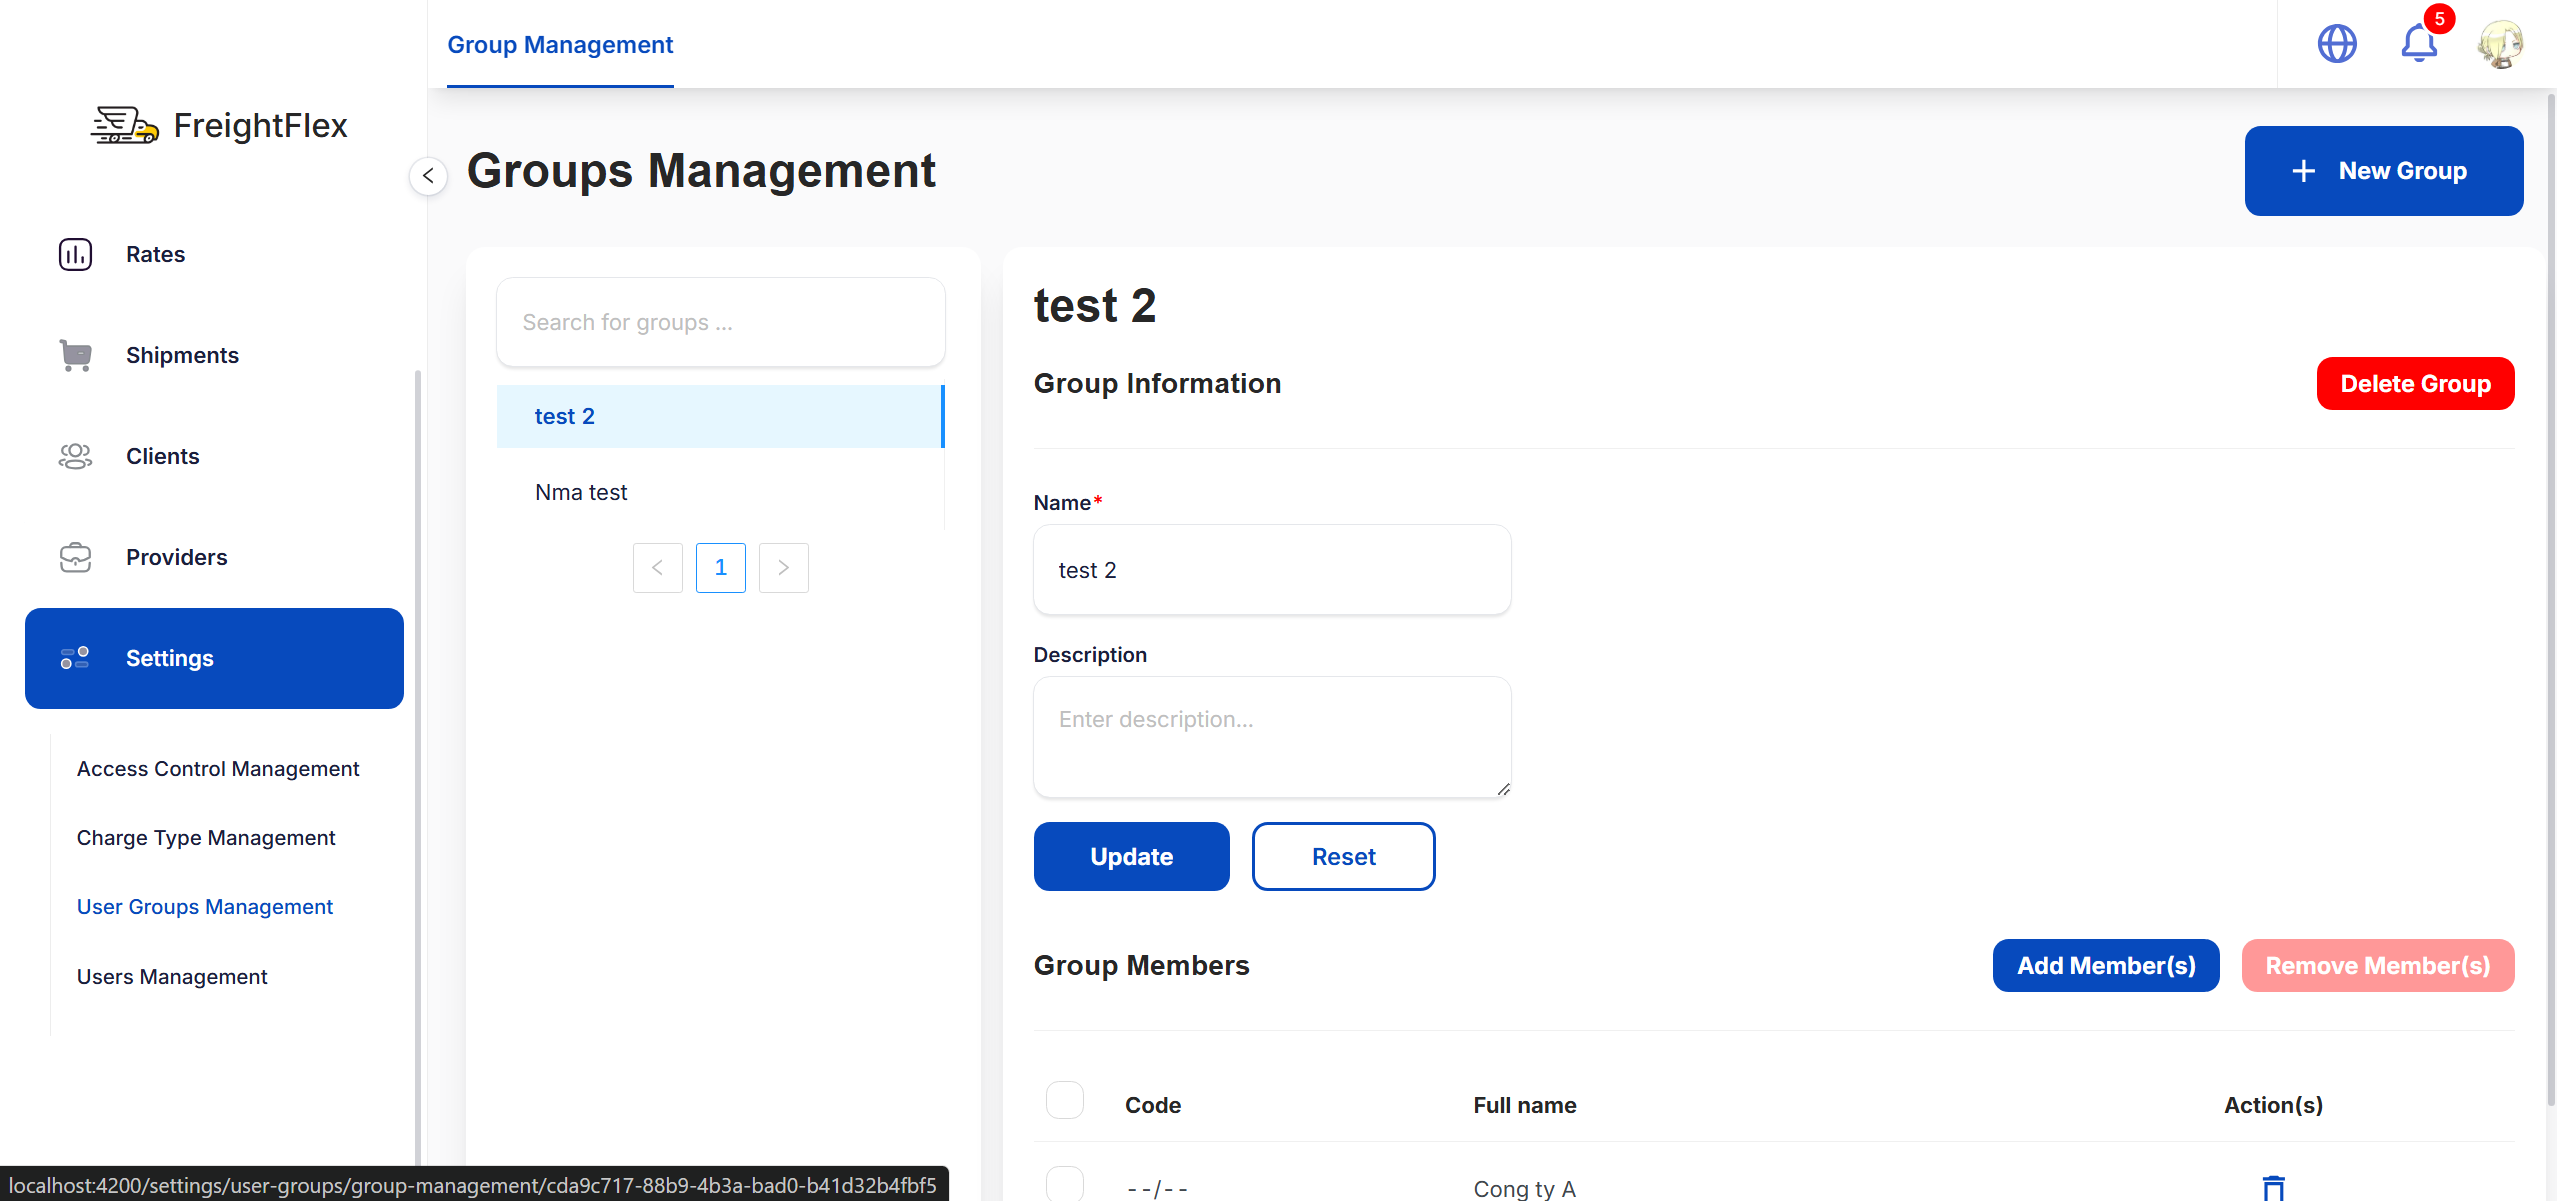
\includegraphics[width=15cm]{graphics/UI/group-management.png}
    \caption{Group Management Overview}
    \label{fig:group-management}
\end{figure}

\begin{figure}[H]
    \centering
    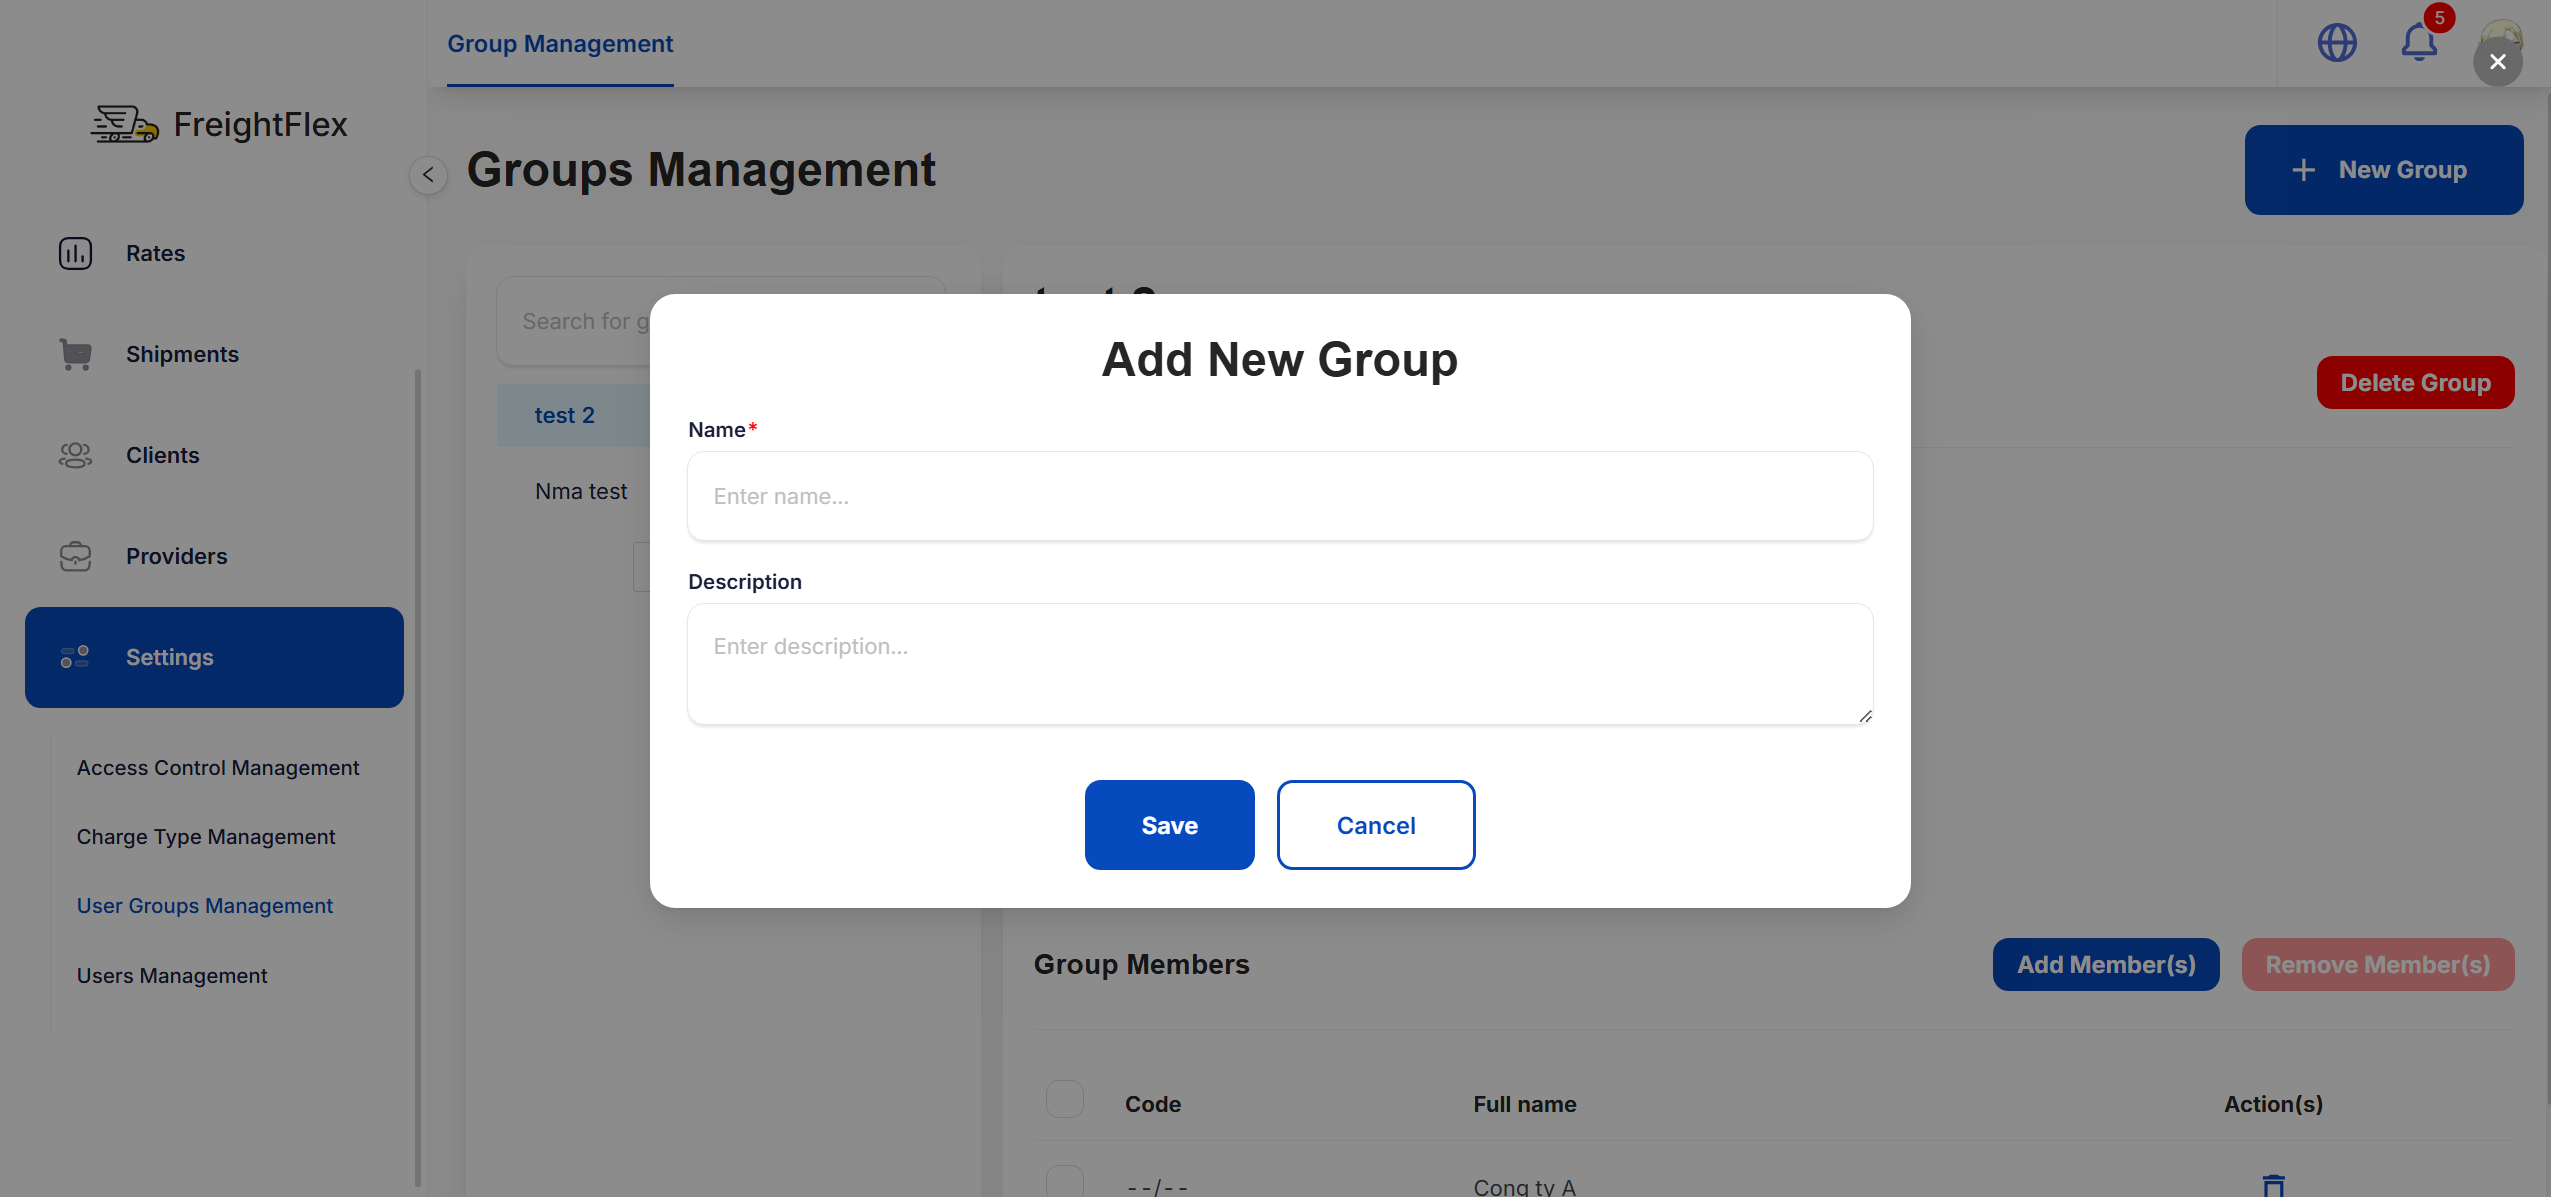
\includegraphics[width=15cm]{graphics/UI/new-group.png}
    \caption{New Group Creation}
    \label{fig:new-group}
\end{figure}

% Provider Management
\begin{figure}[H]
    \centering
    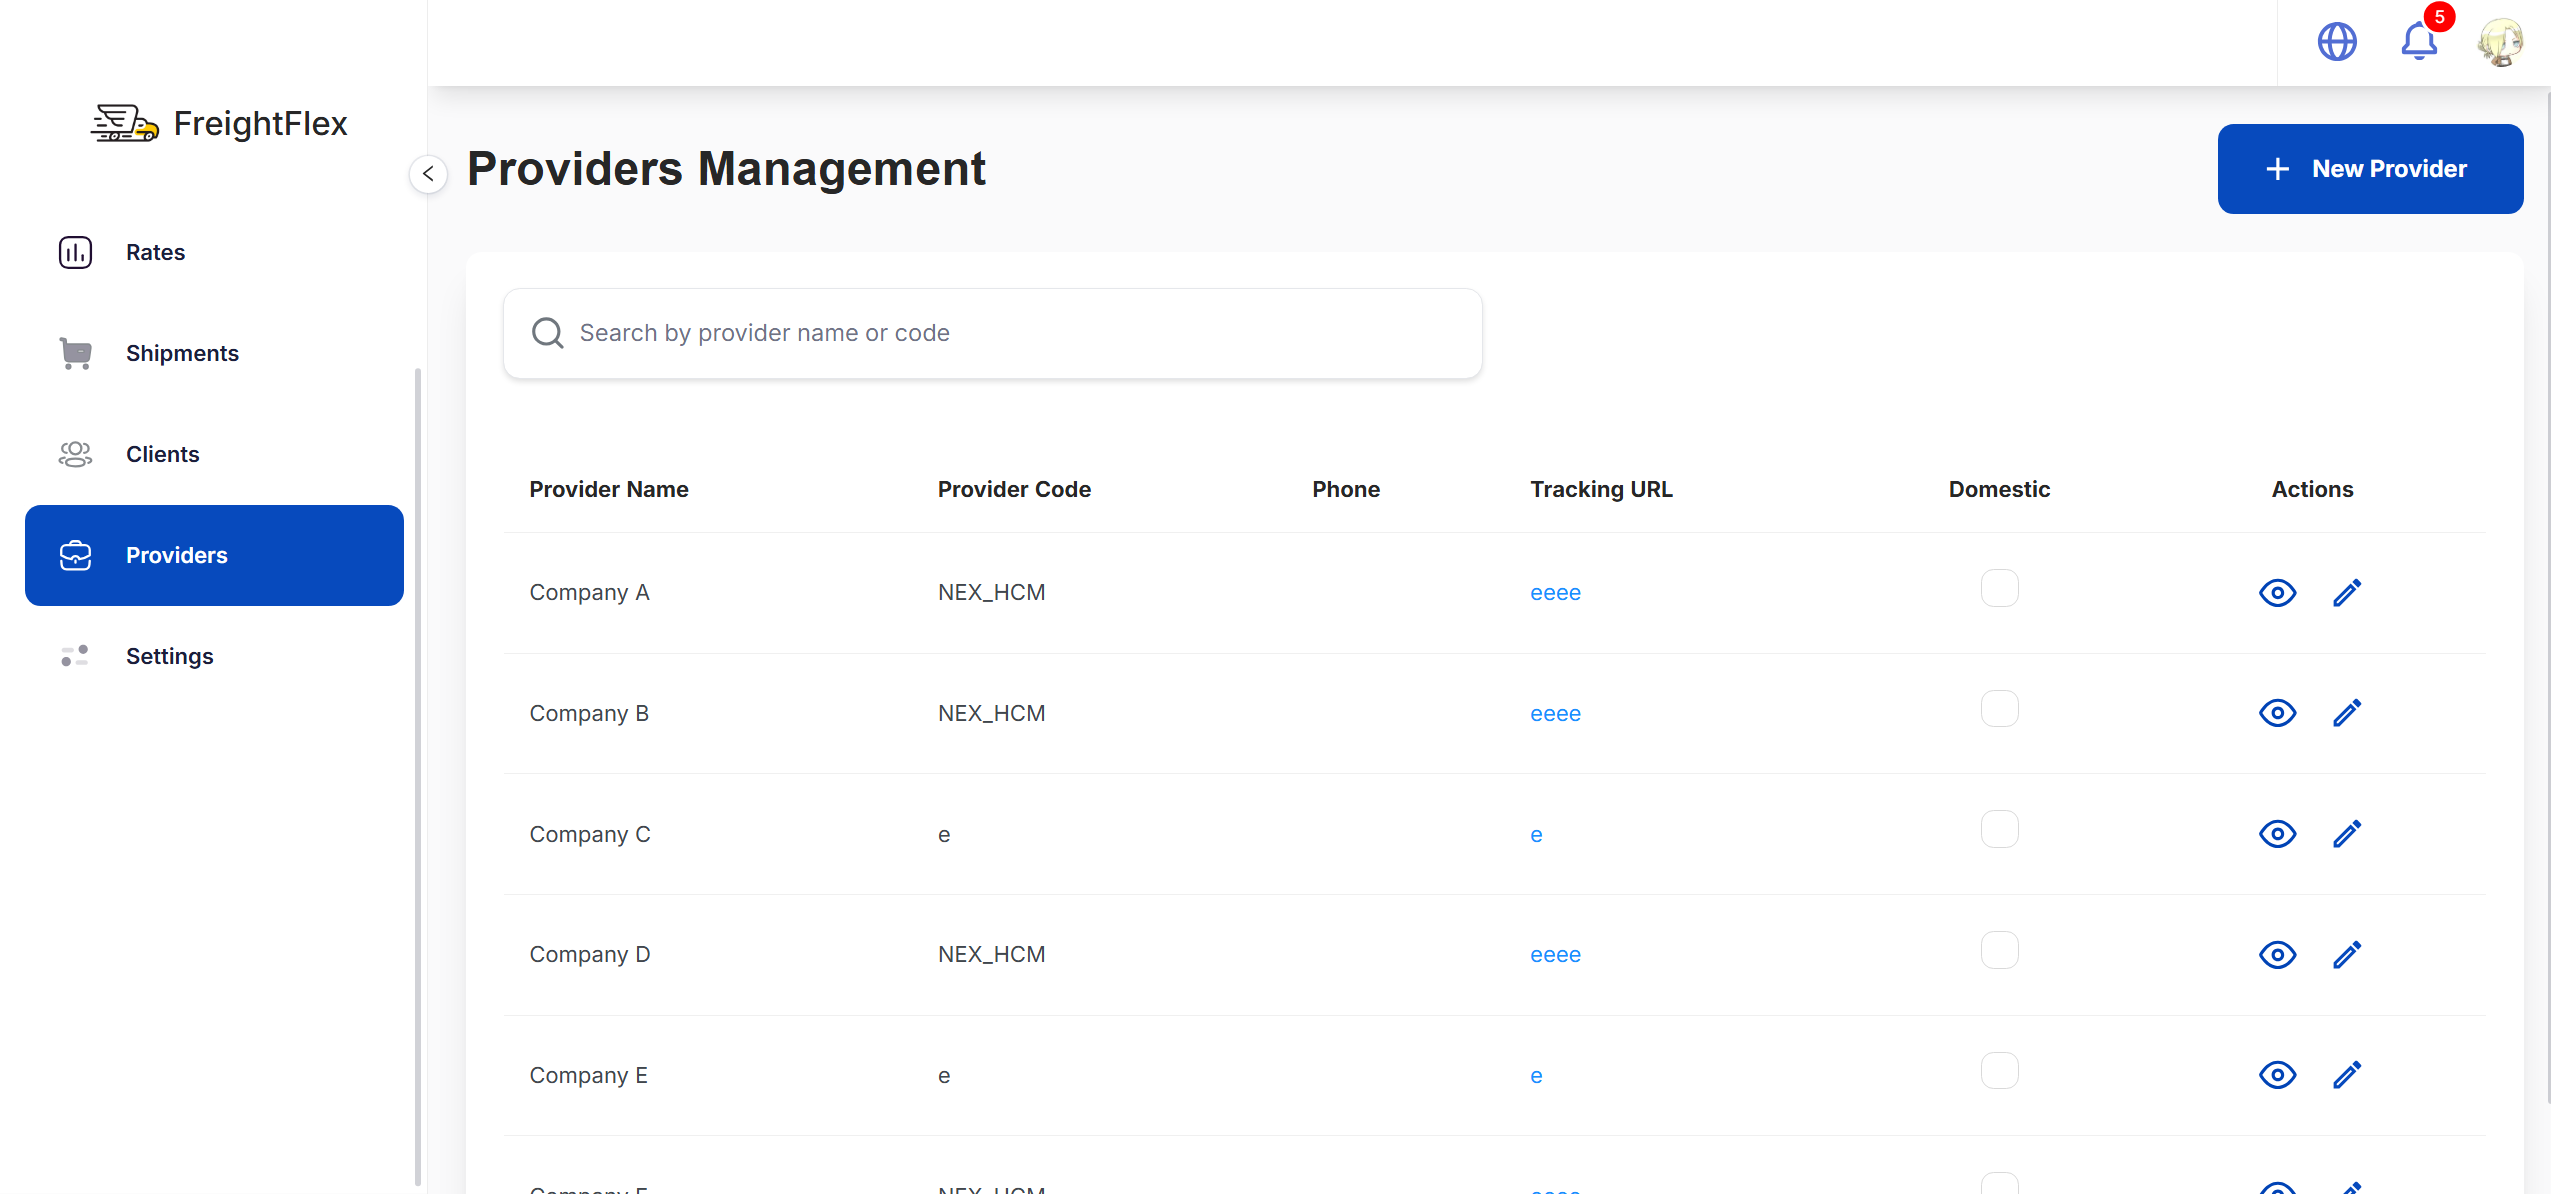
\includegraphics[width=15cm]{graphics/UI/provider-management.png}
    \caption{Provider Management Overview}
    \label{fig:provider-management}
\end{figure}

\begin{figure}[H]
    \centering
    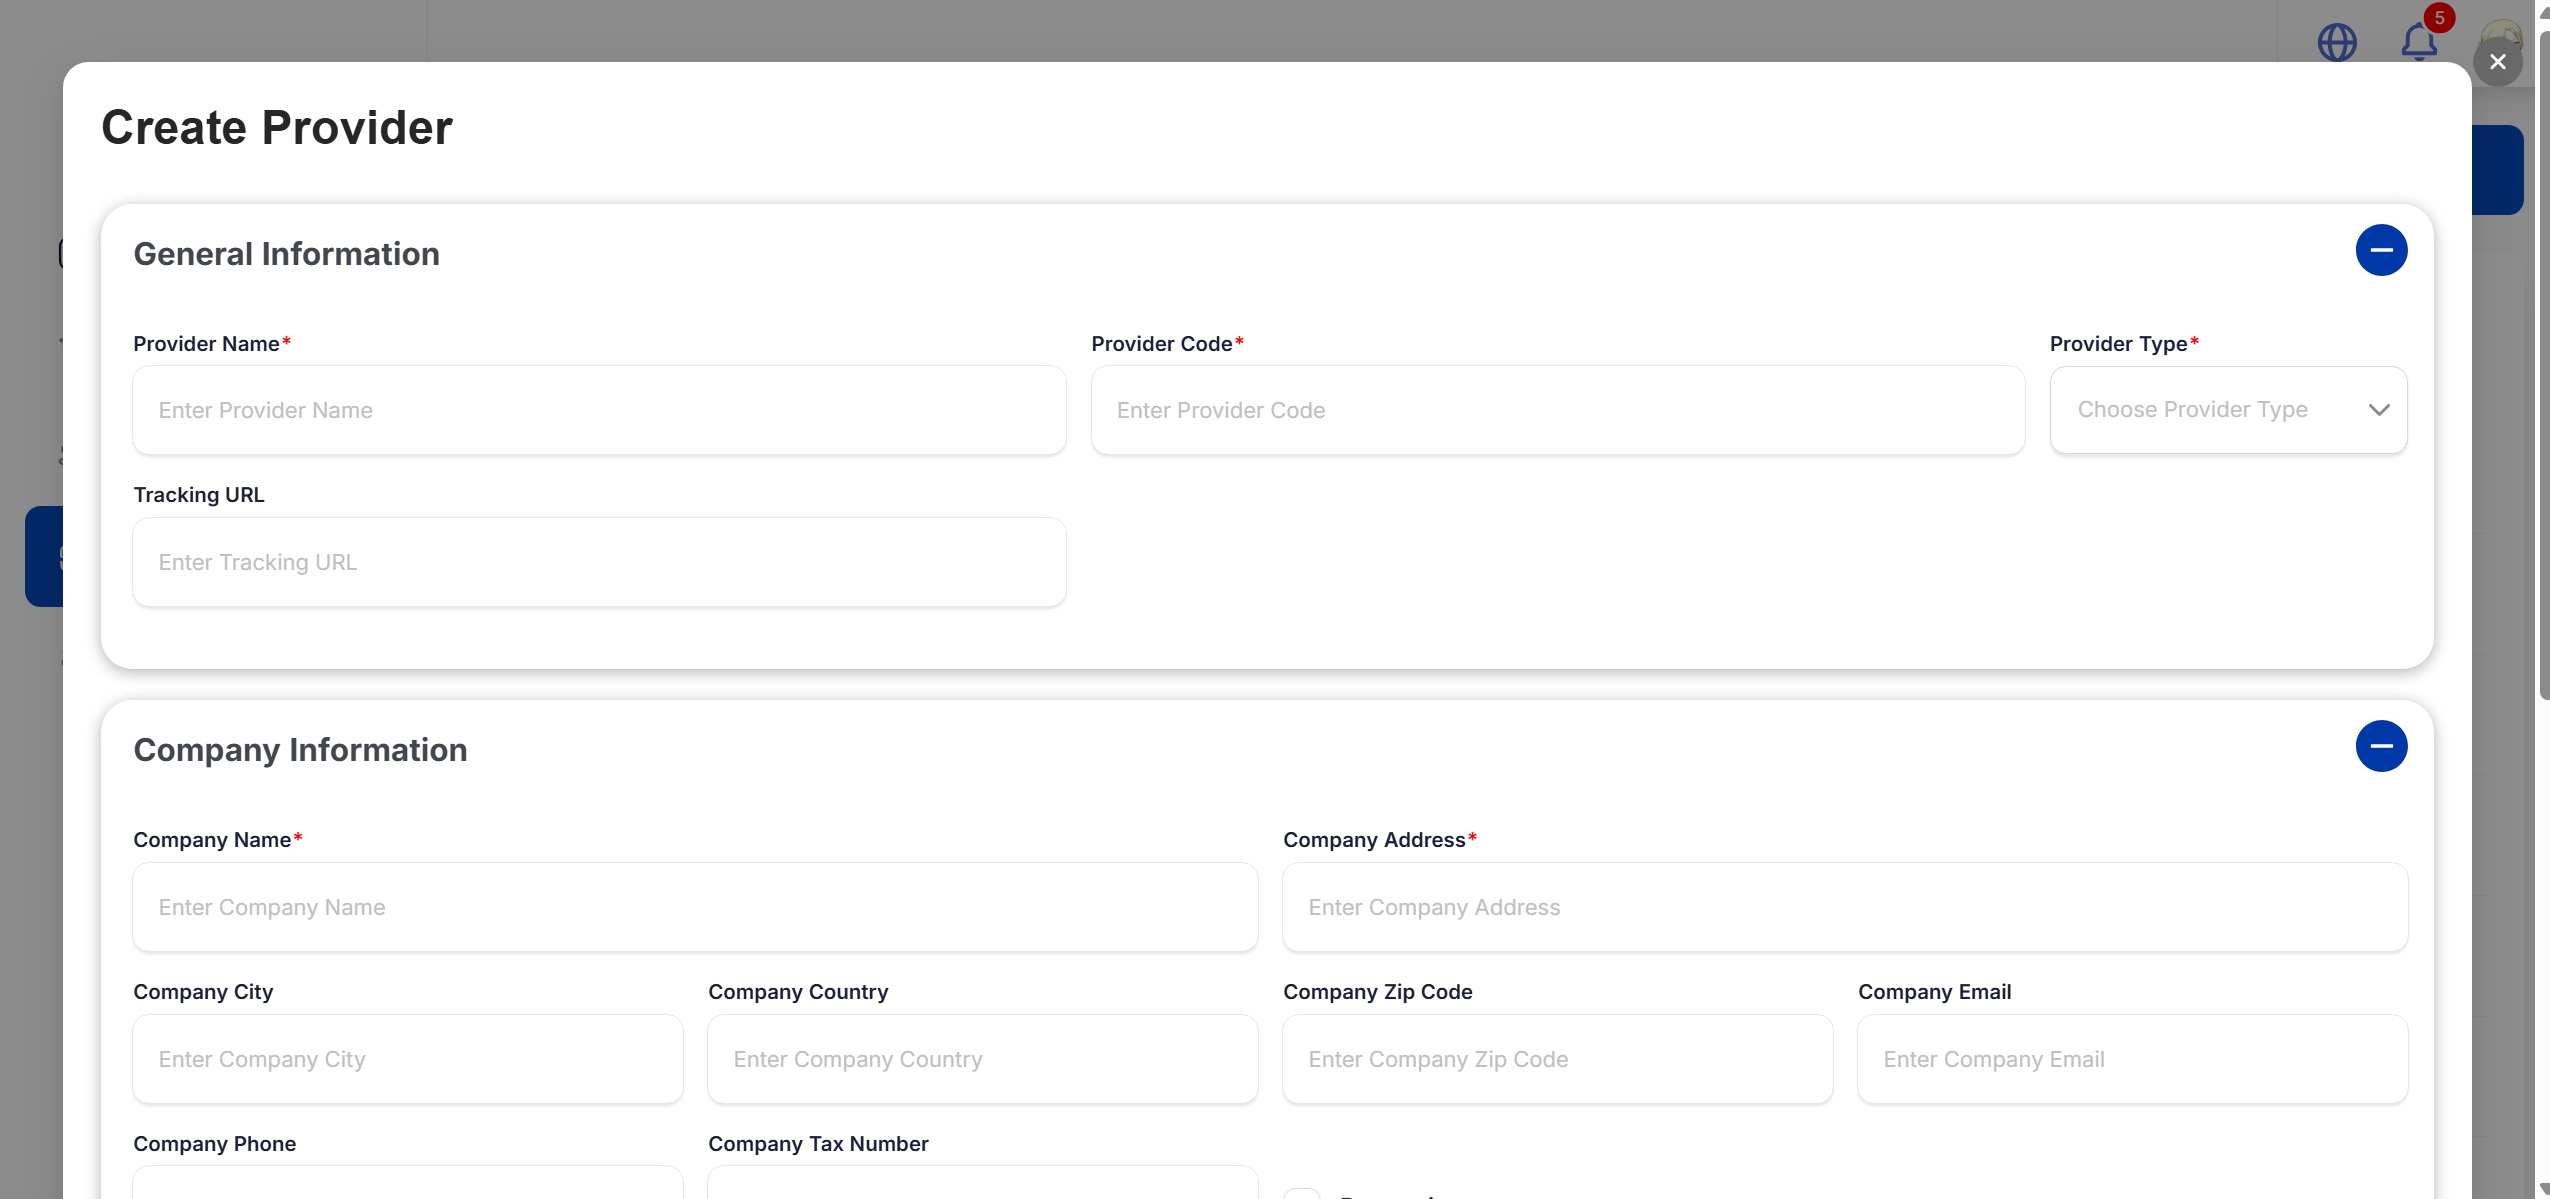
\includegraphics[width=15cm]{graphics/UI/new-provider.png}
    \caption{New Provider Registration}
    \label{fig:new-provider}
\end{figure}

% Charge and Rate Management
\begin{figure}[H]
    \centering
    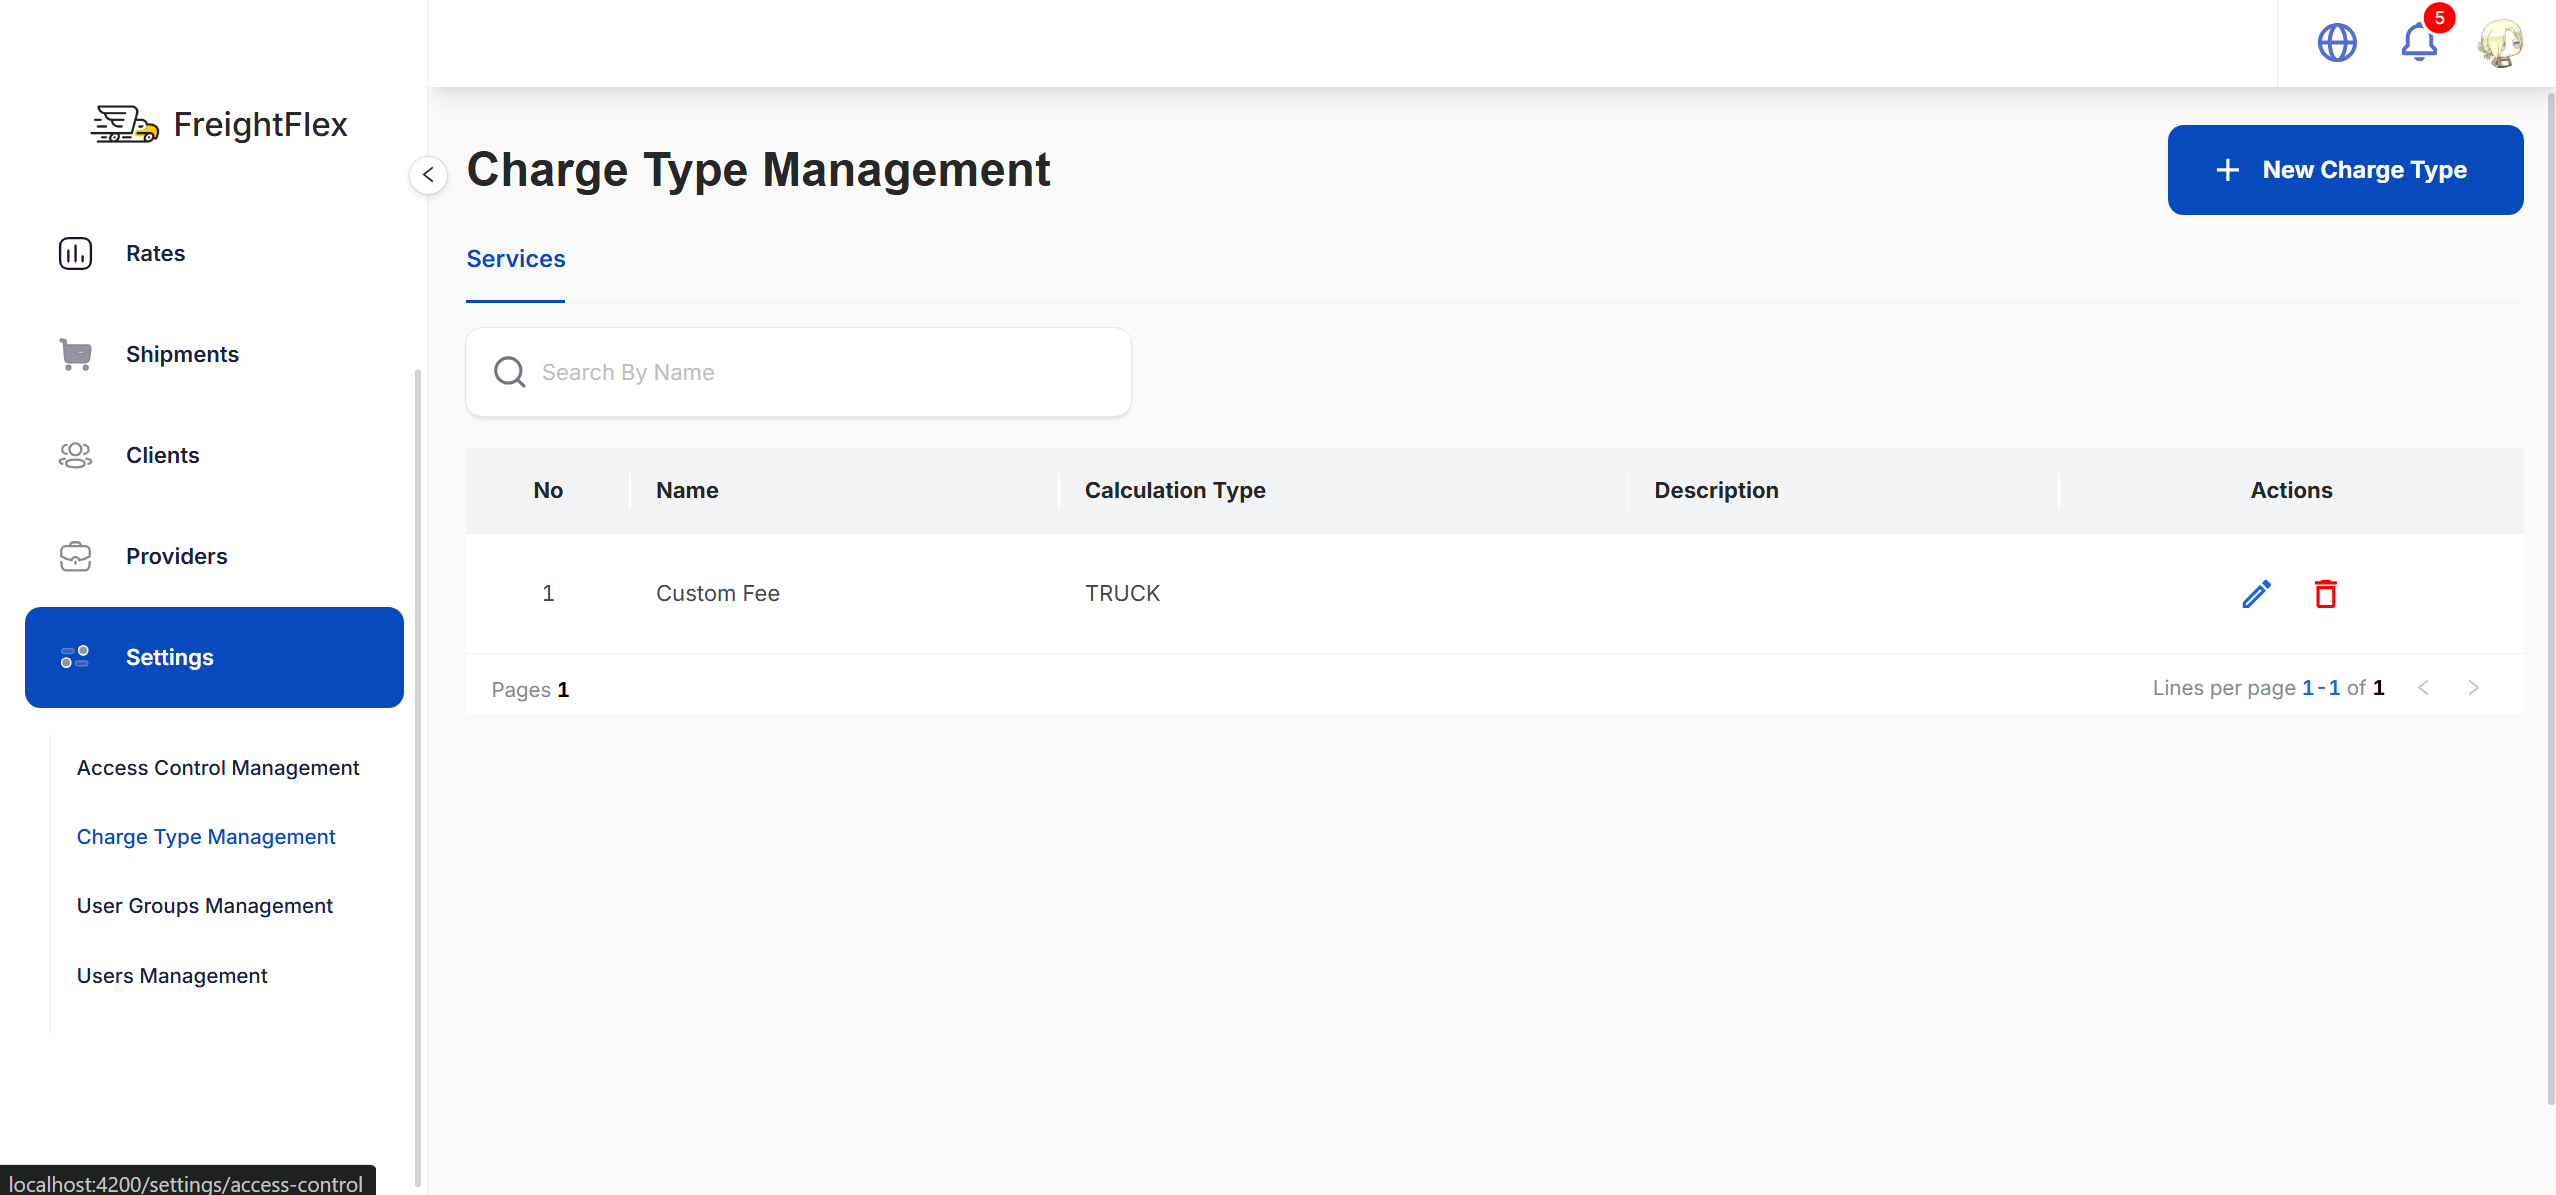
\includegraphics[width=15cm]{graphics/UI/charge-type-management.png}
    \caption{Charge Type Management}
    \label{fig:charge-type-management}
\end{figure}

\begin{figure}[H]
    \centering
    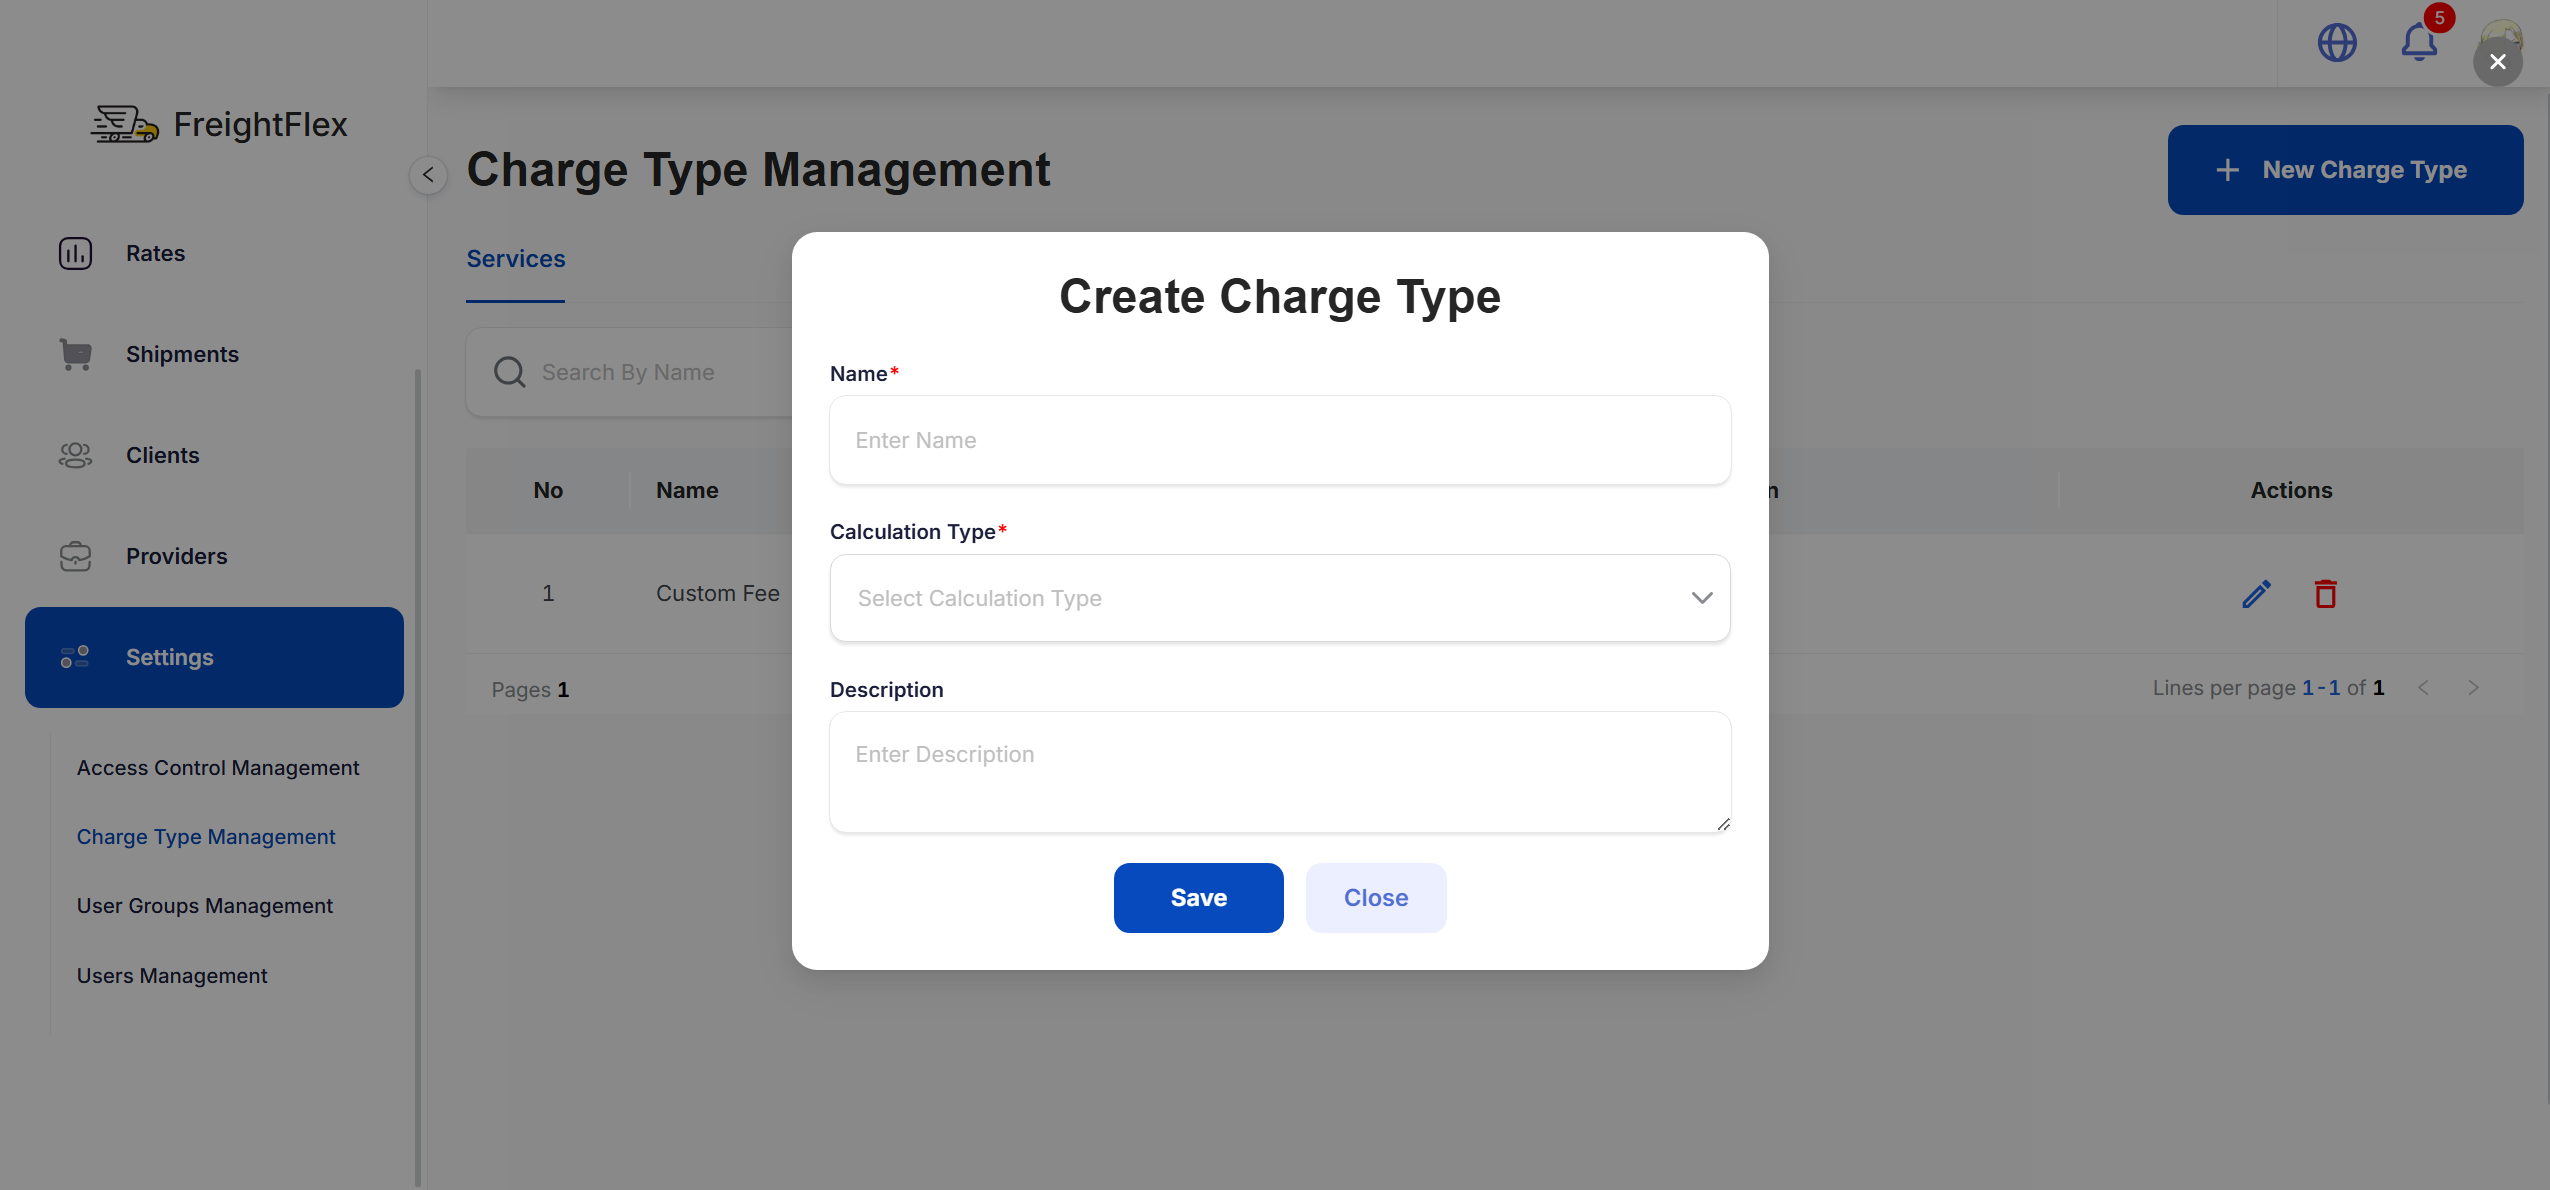
\includegraphics[width=15cm]{graphics/UI/new-charge-type.png}
    \caption{New Charge Type Creation}
    \label{fig:new-charge-type}
\end{figure}

\begin{figure}[H]
    \centering
    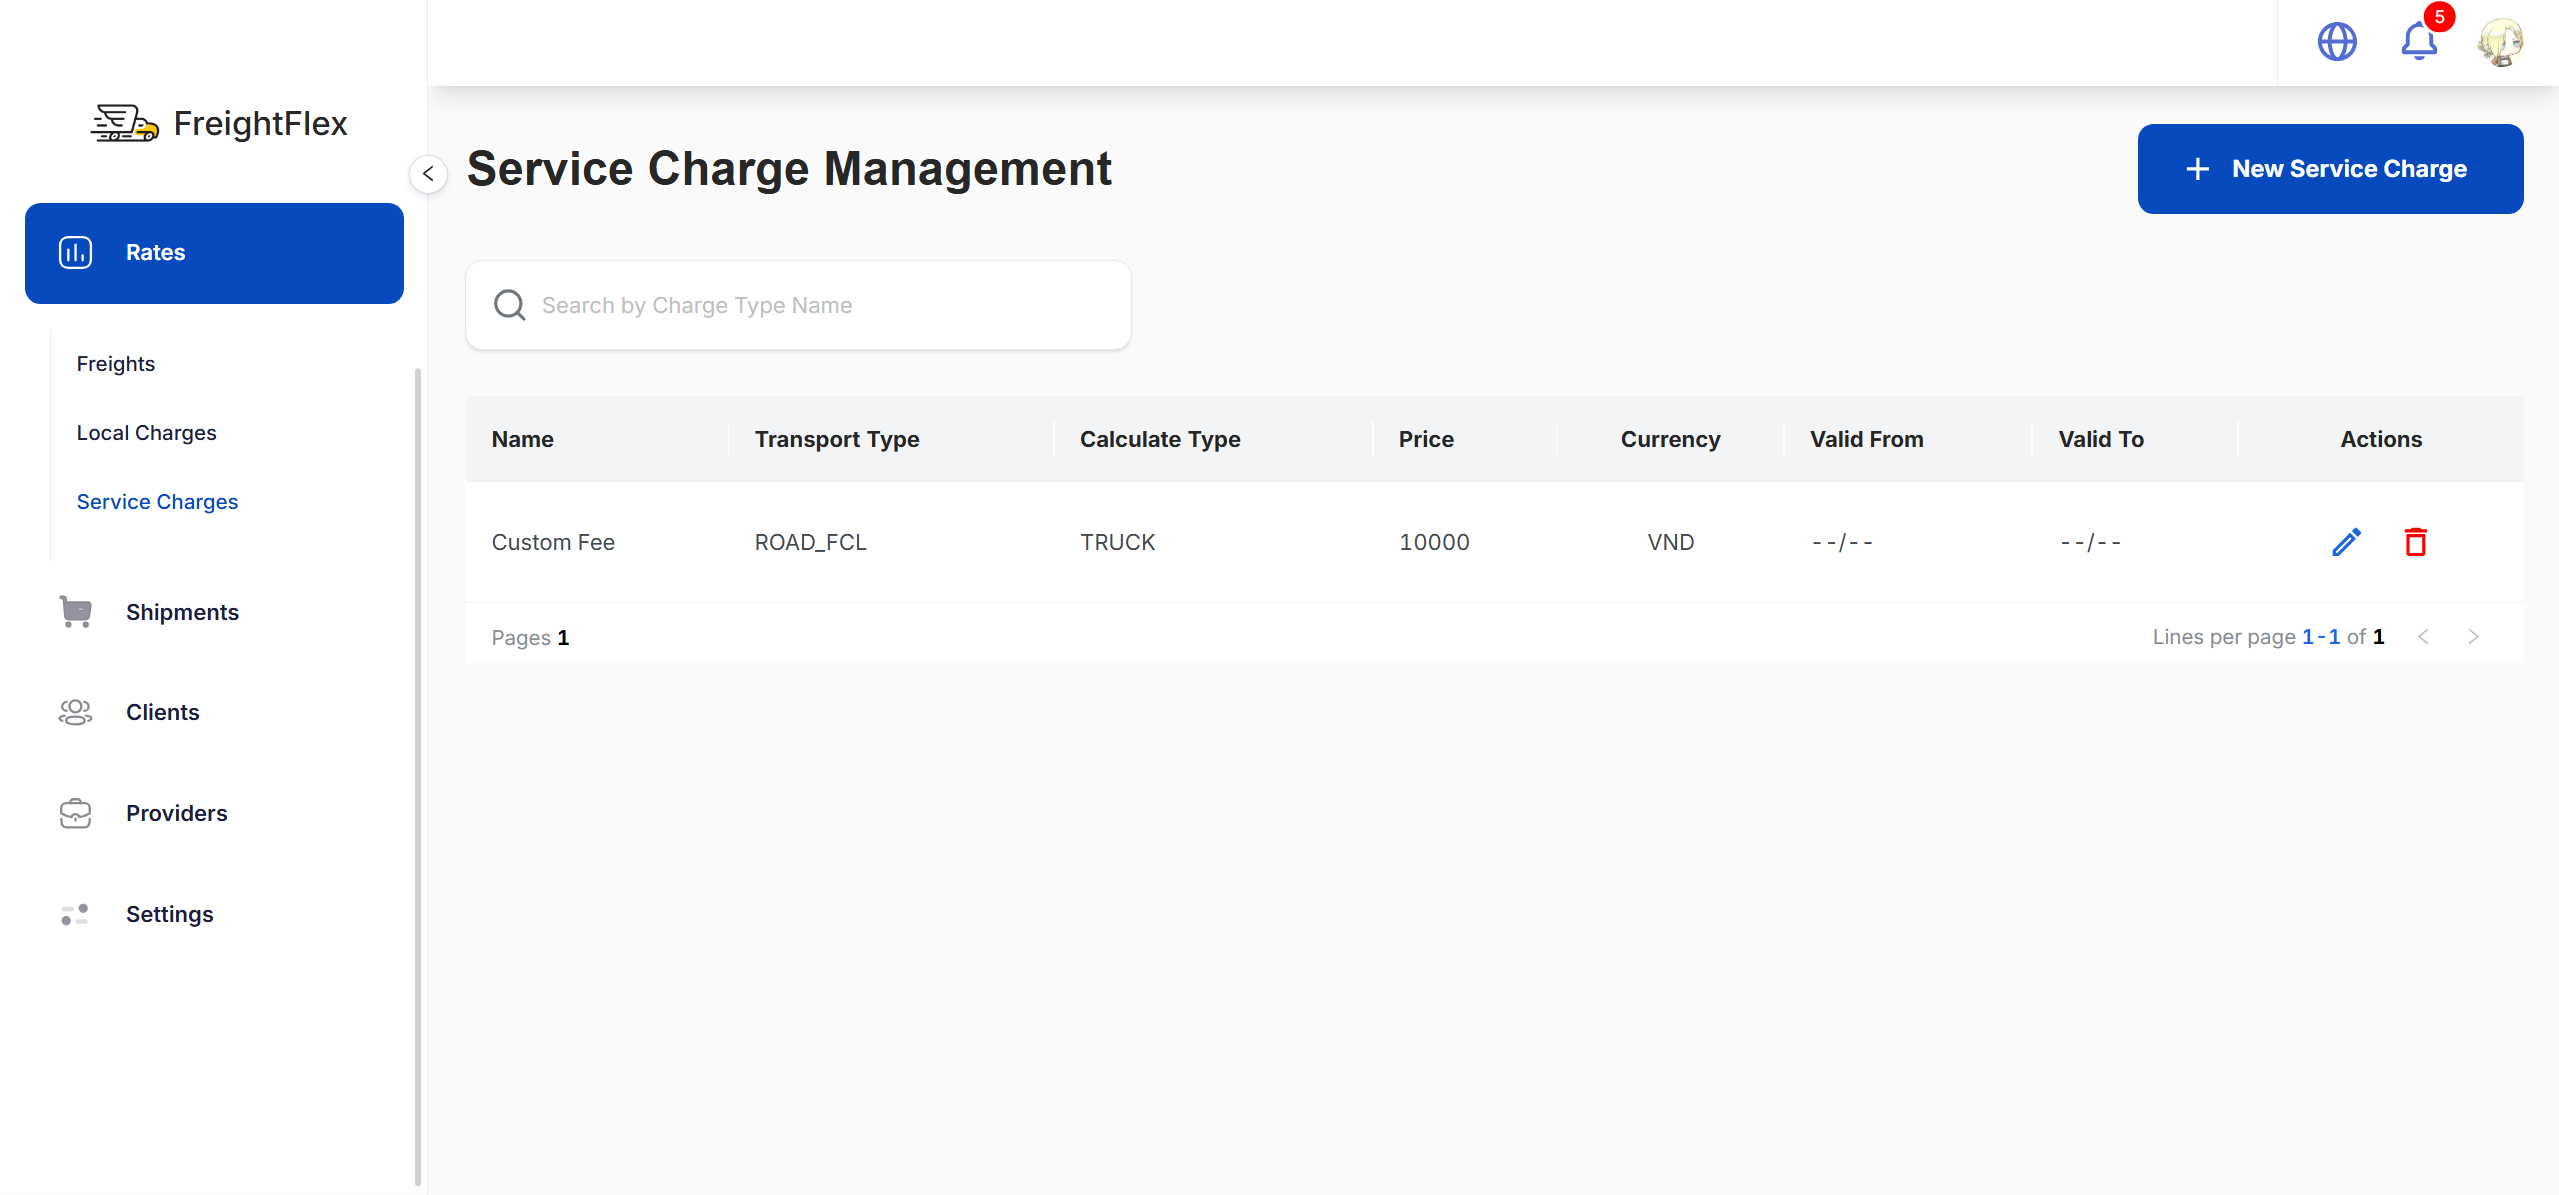
\includegraphics[width=15cm]{graphics/UI/service-charge-management.png}
    \caption{Service Charge Management}
    \label{fig:service-charge-management}
\end{figure}

\begin{figure}[H]
    \centering
    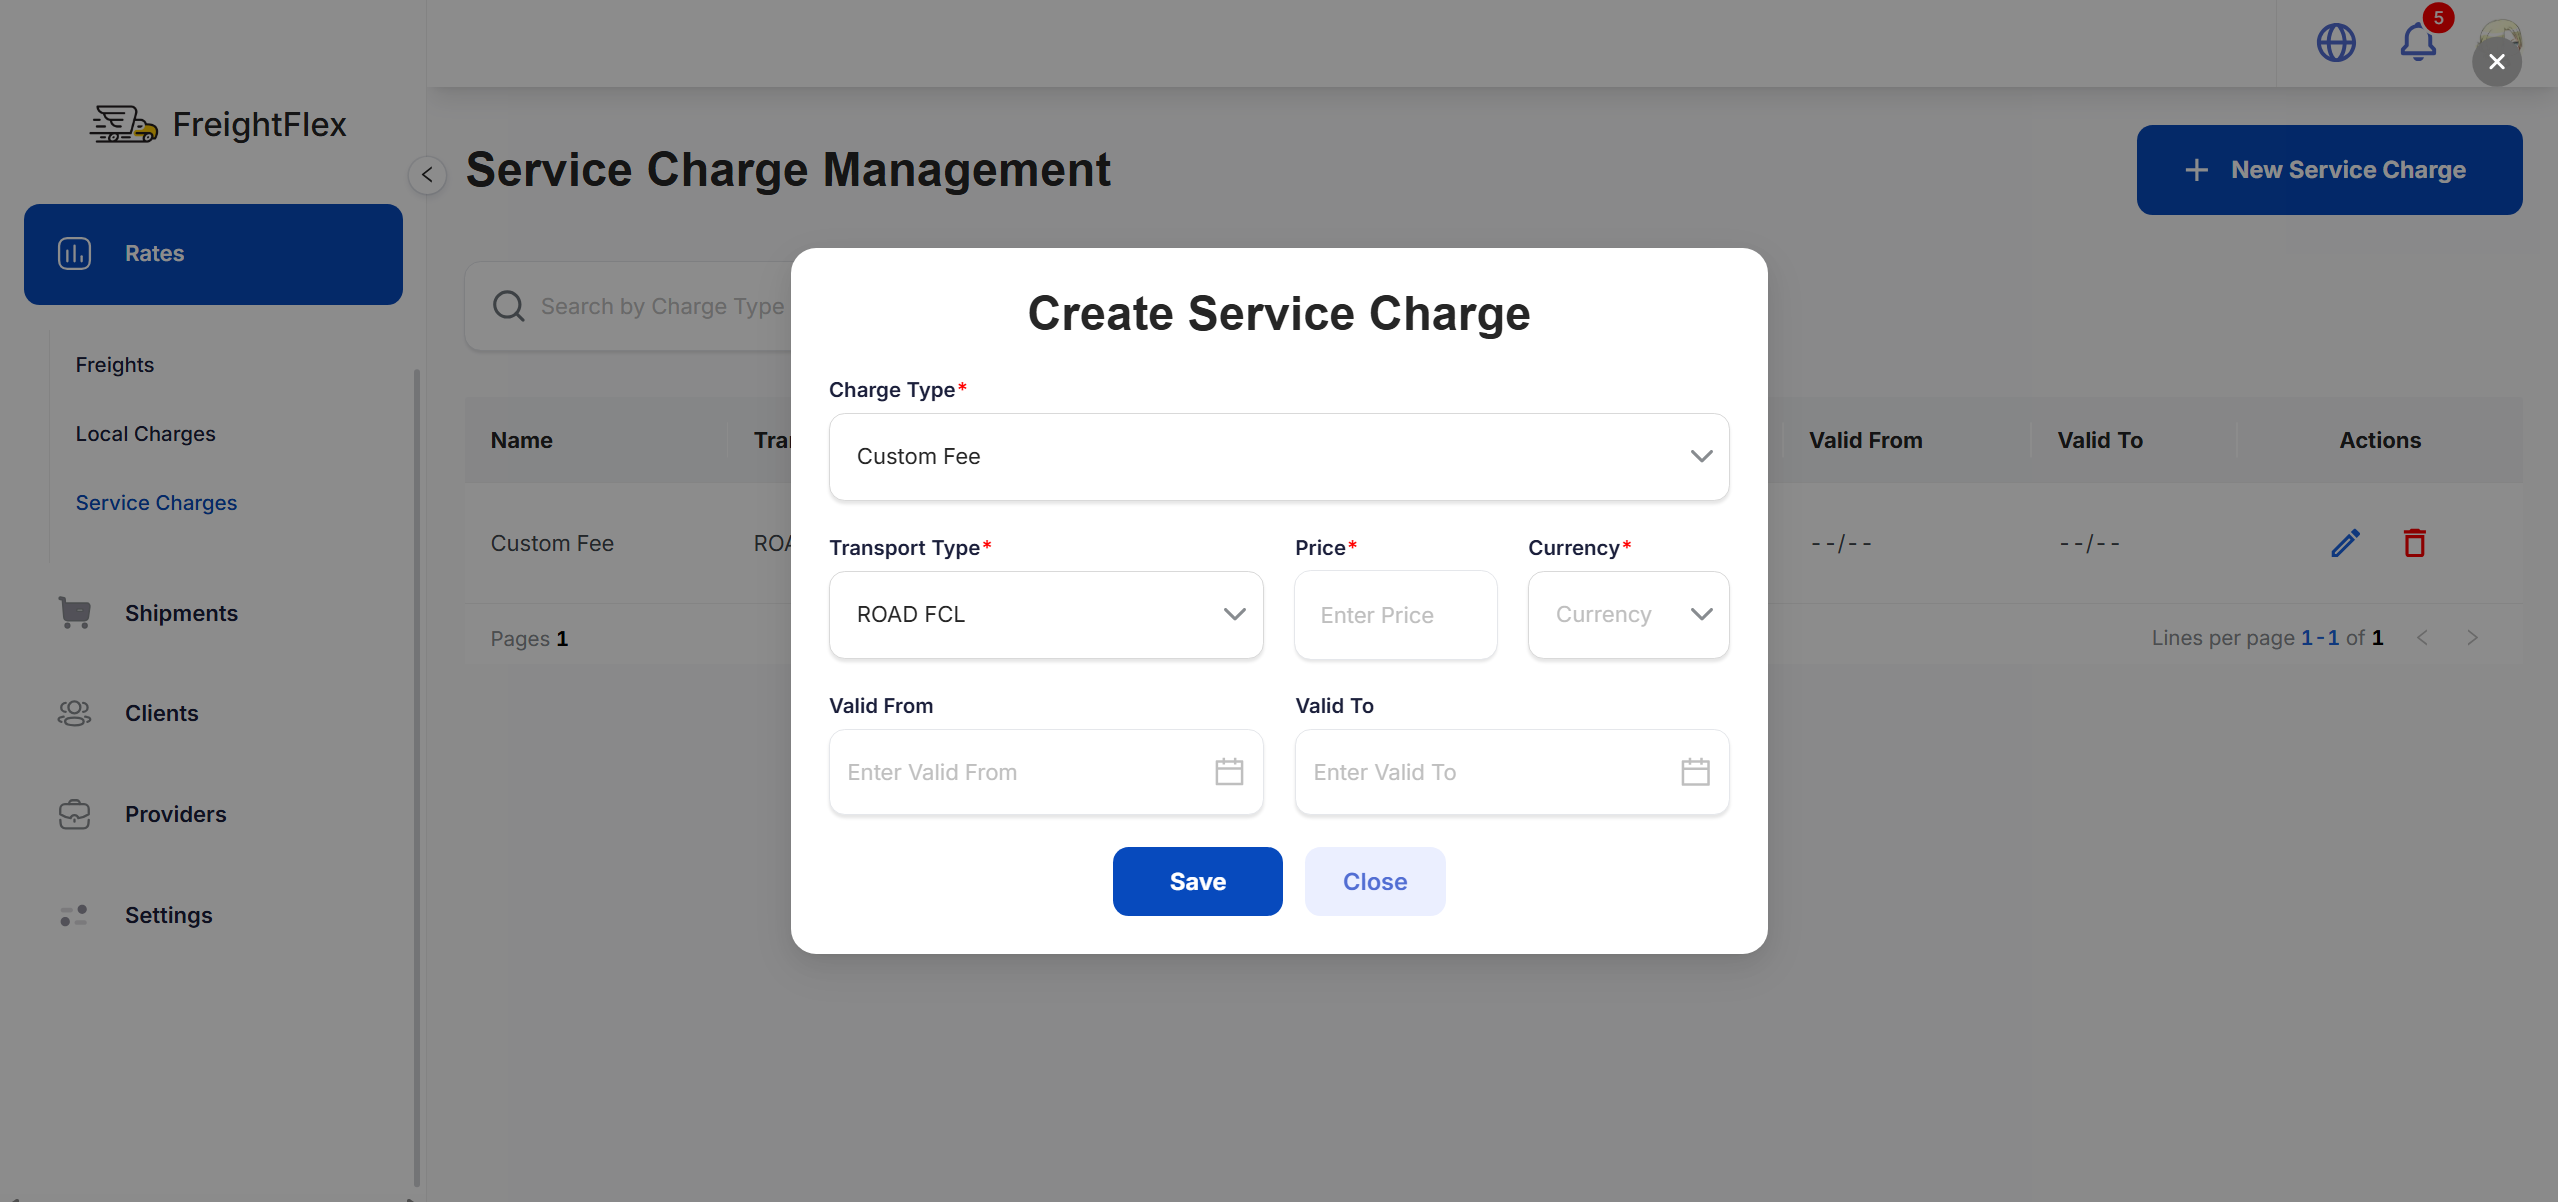
\includegraphics[width=15cm]{graphics/UI/new-service-charge.png}
    \caption{New Service Charge Creation}
    \label{fig:new-service-charge}
\end{figure}

\begin{figure}[H]
    \centering
    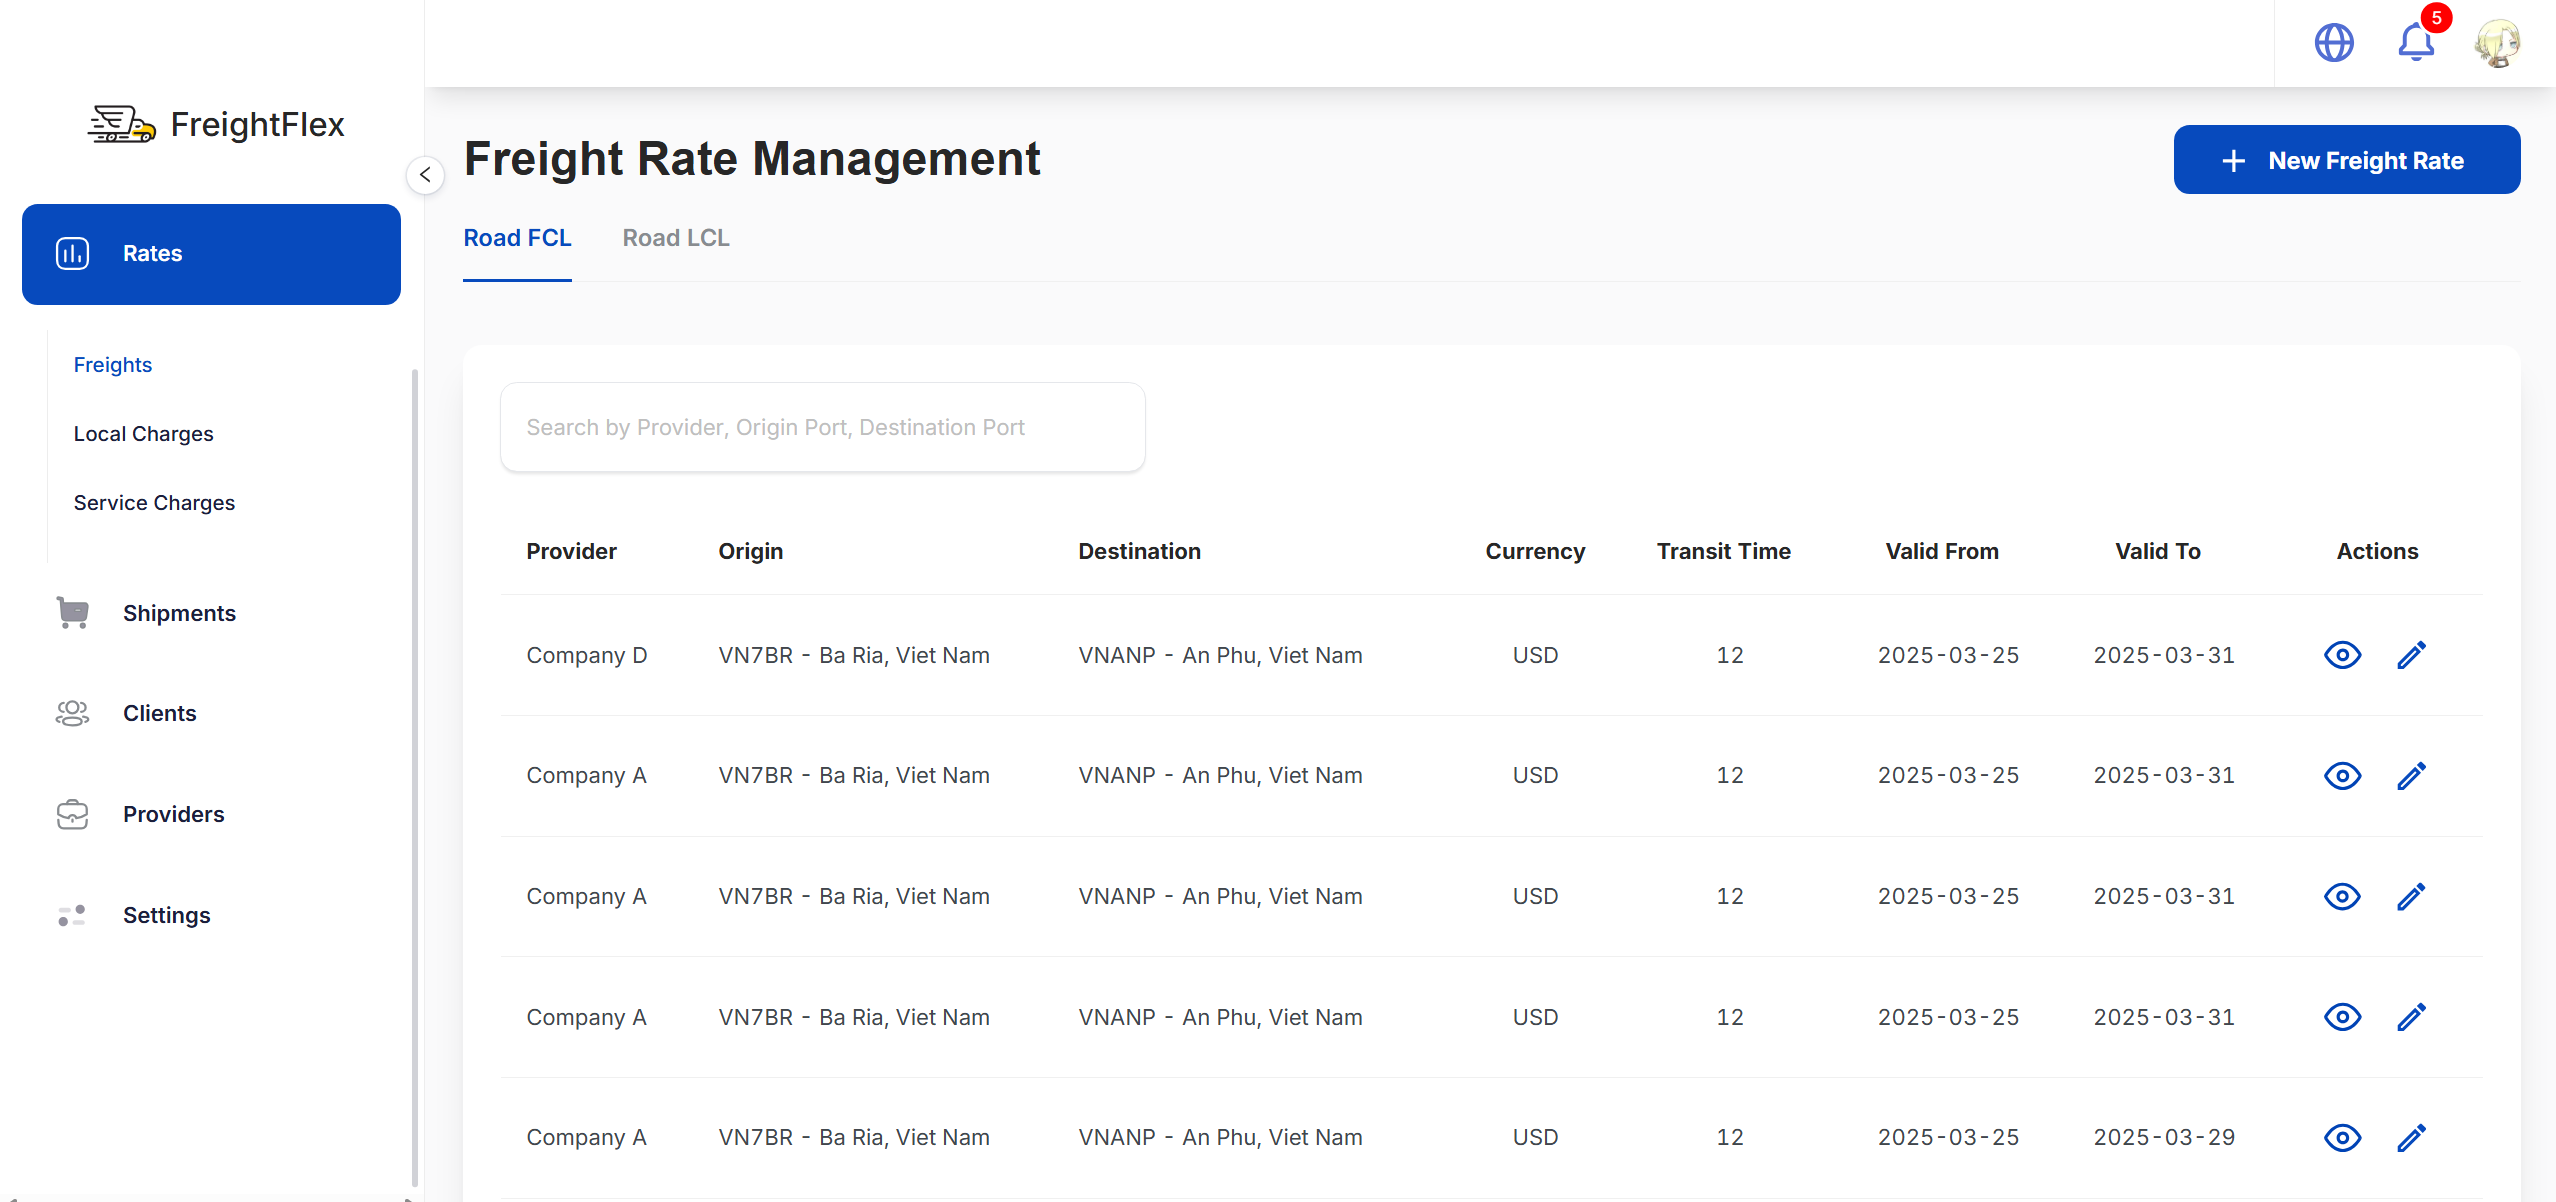
\includegraphics[width=15cm]{graphics/UI/rate-management.png}
    \caption{Rate Management}
    \label{fig:rate-management}
\end{figure}

\begin{figure}[H]
    \centering
    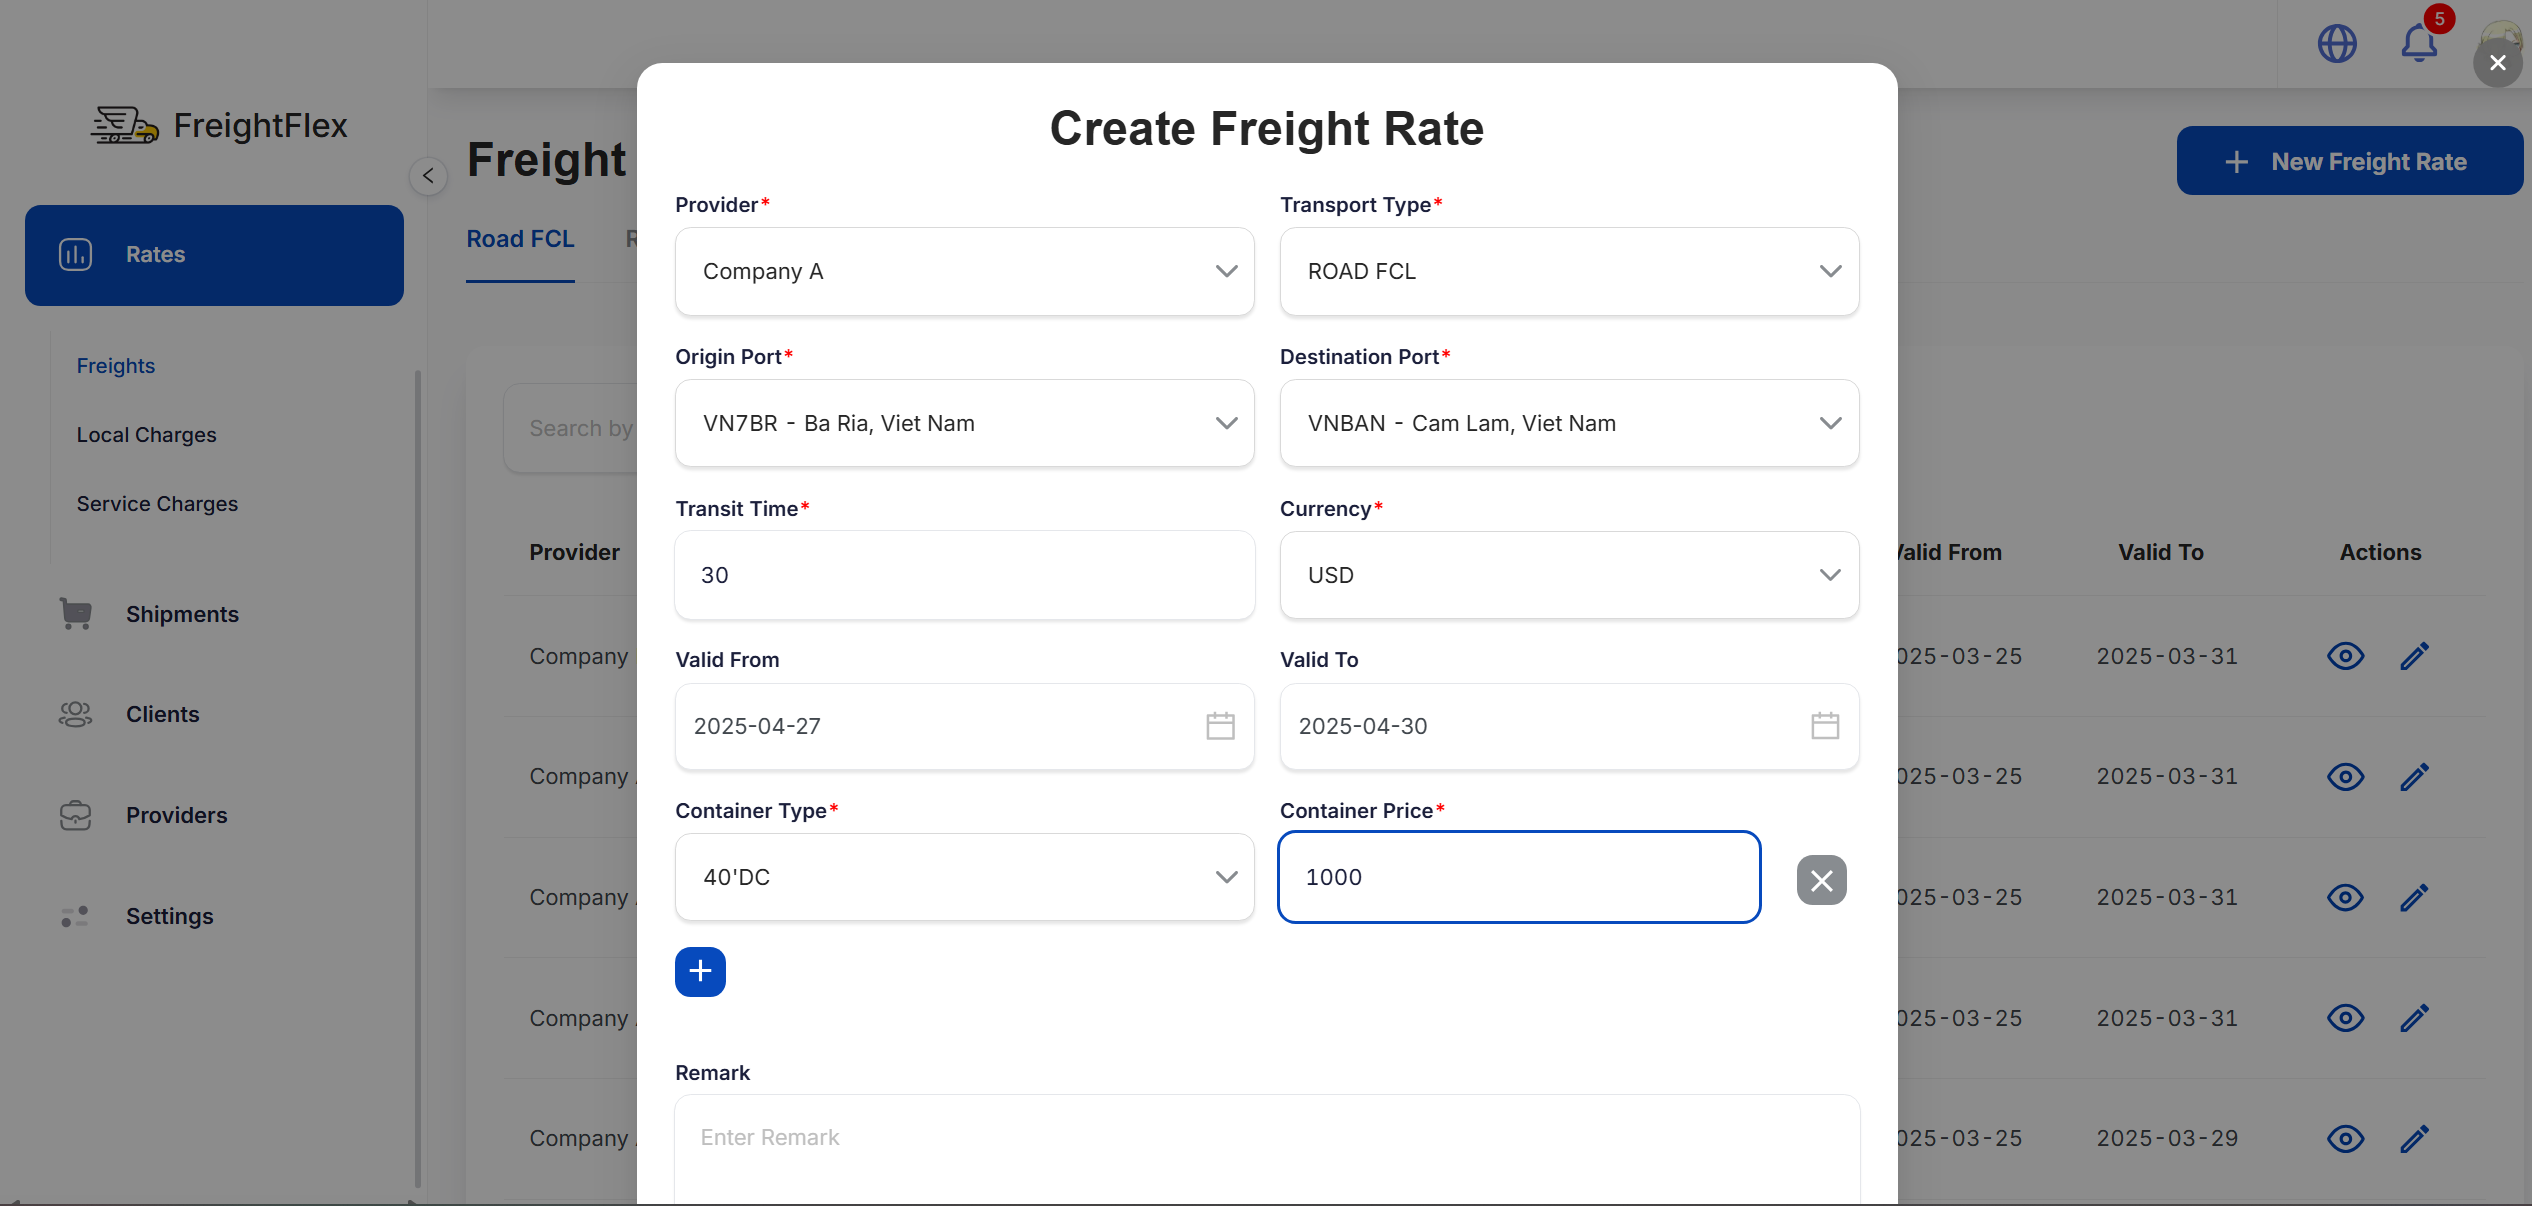
\includegraphics[width=15cm]{graphics/UI/new-freight-rate.png}
    \caption{New Freight Rate Creation}
    \label{fig:new-freight-rate}
\end{figure}

% Shipment and Quote Management
\begin{figure}[H]
    \centering
    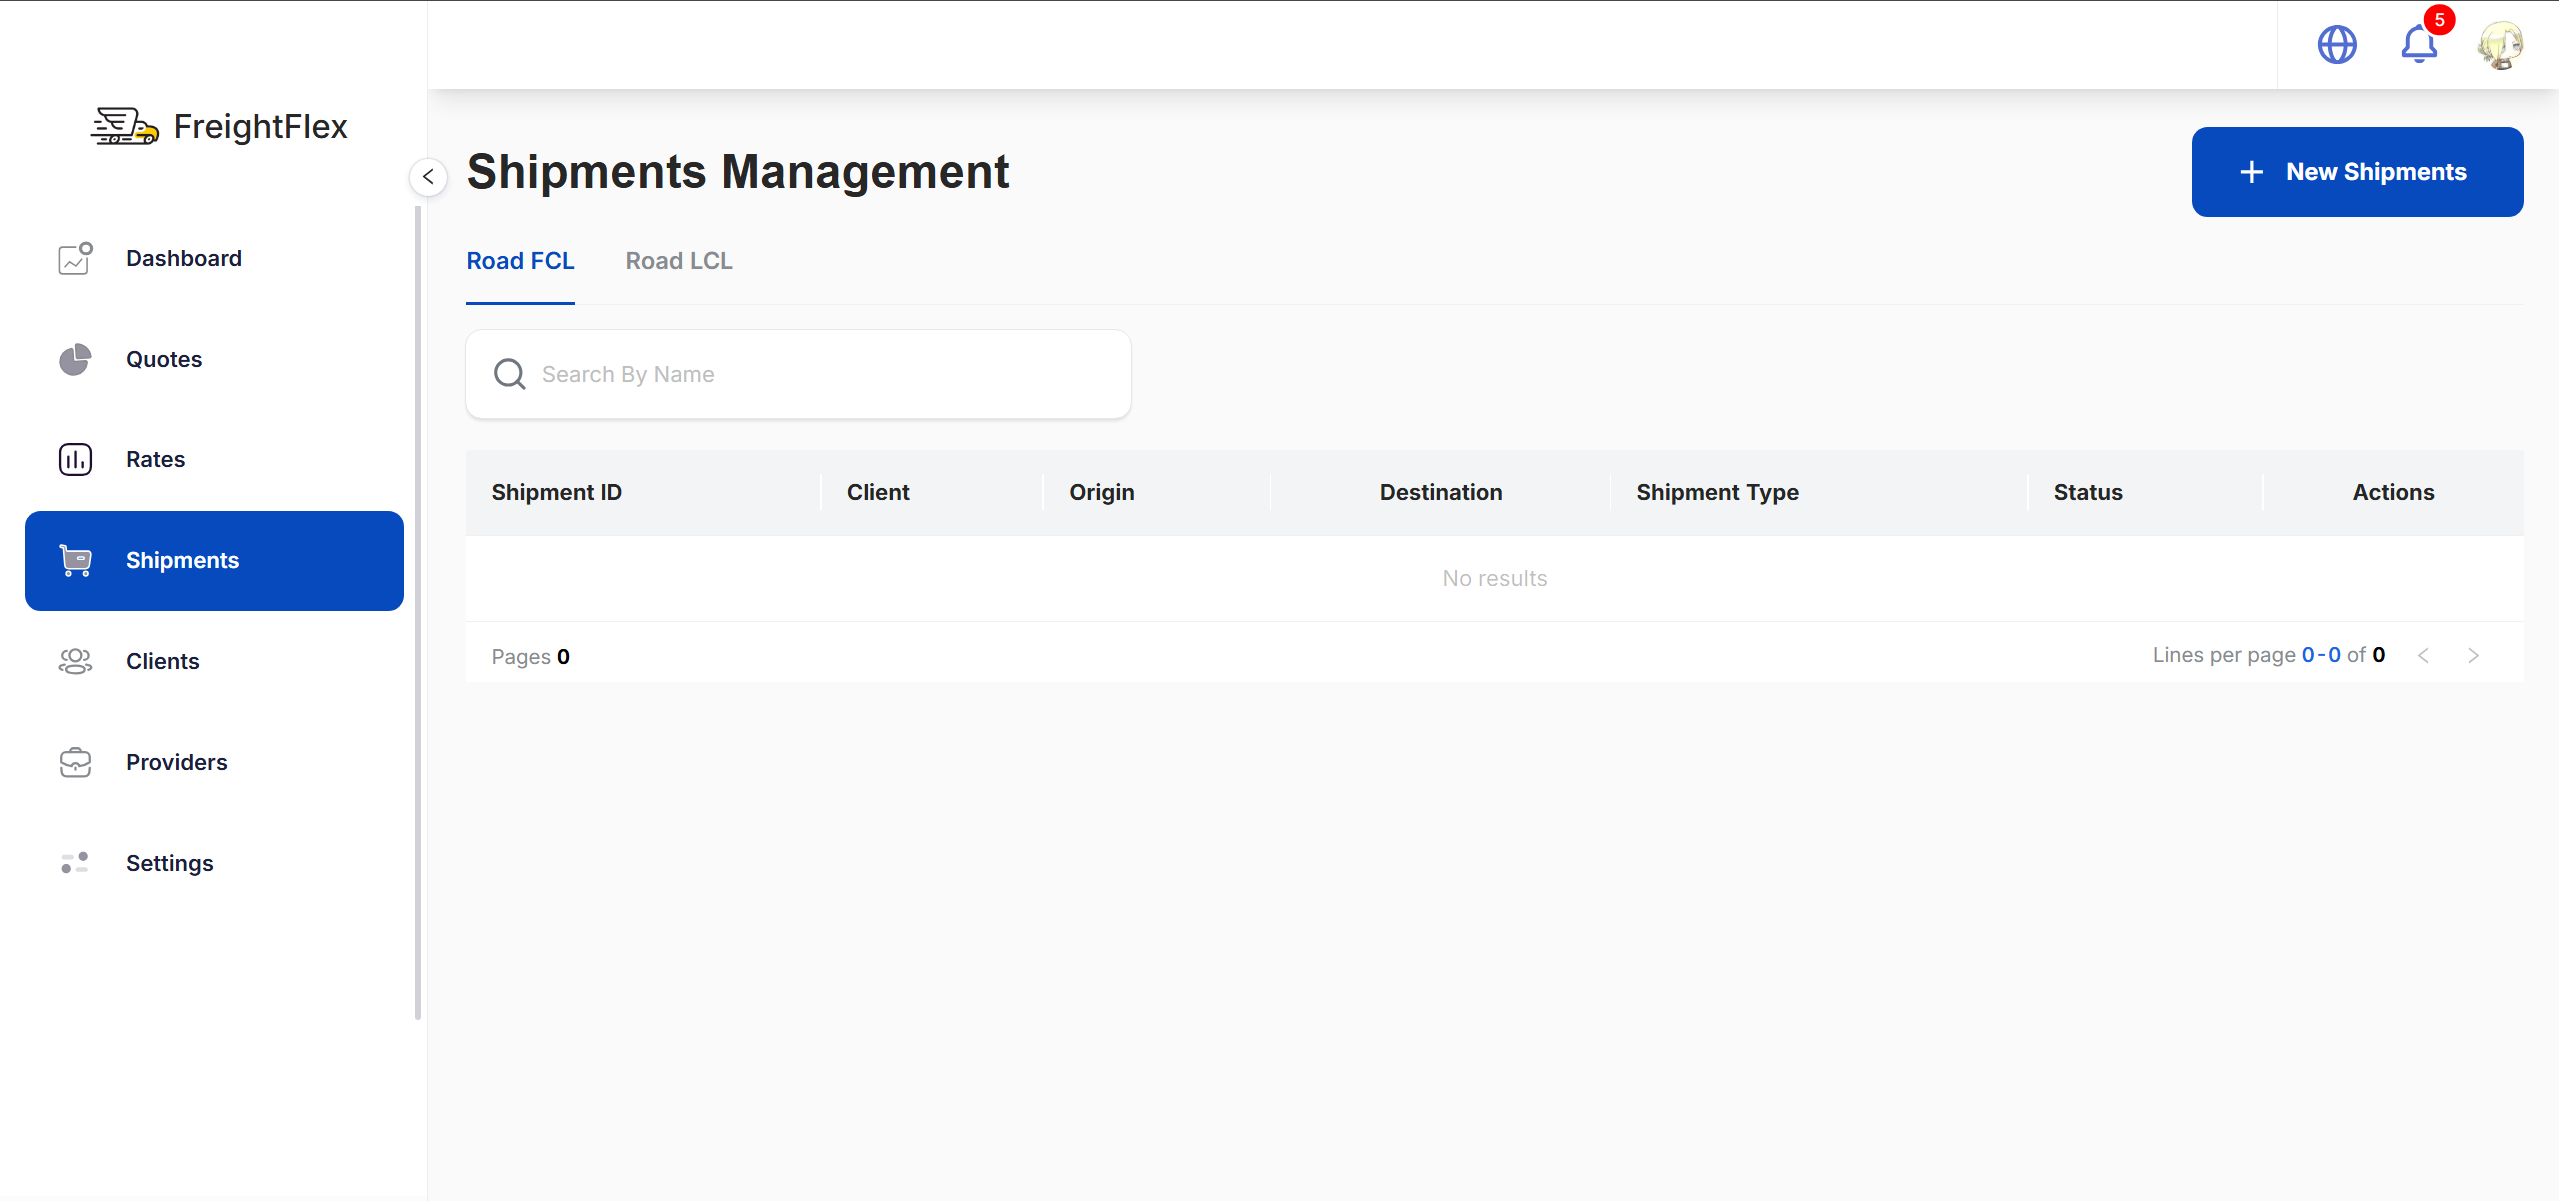
\includegraphics[width=15cm]{graphics/UI/shipment-management.png}
    \caption{Shipment Management}
    \label{fig:shipment-management}
\end{figure}

\begin{figure}[H]
    \centering
    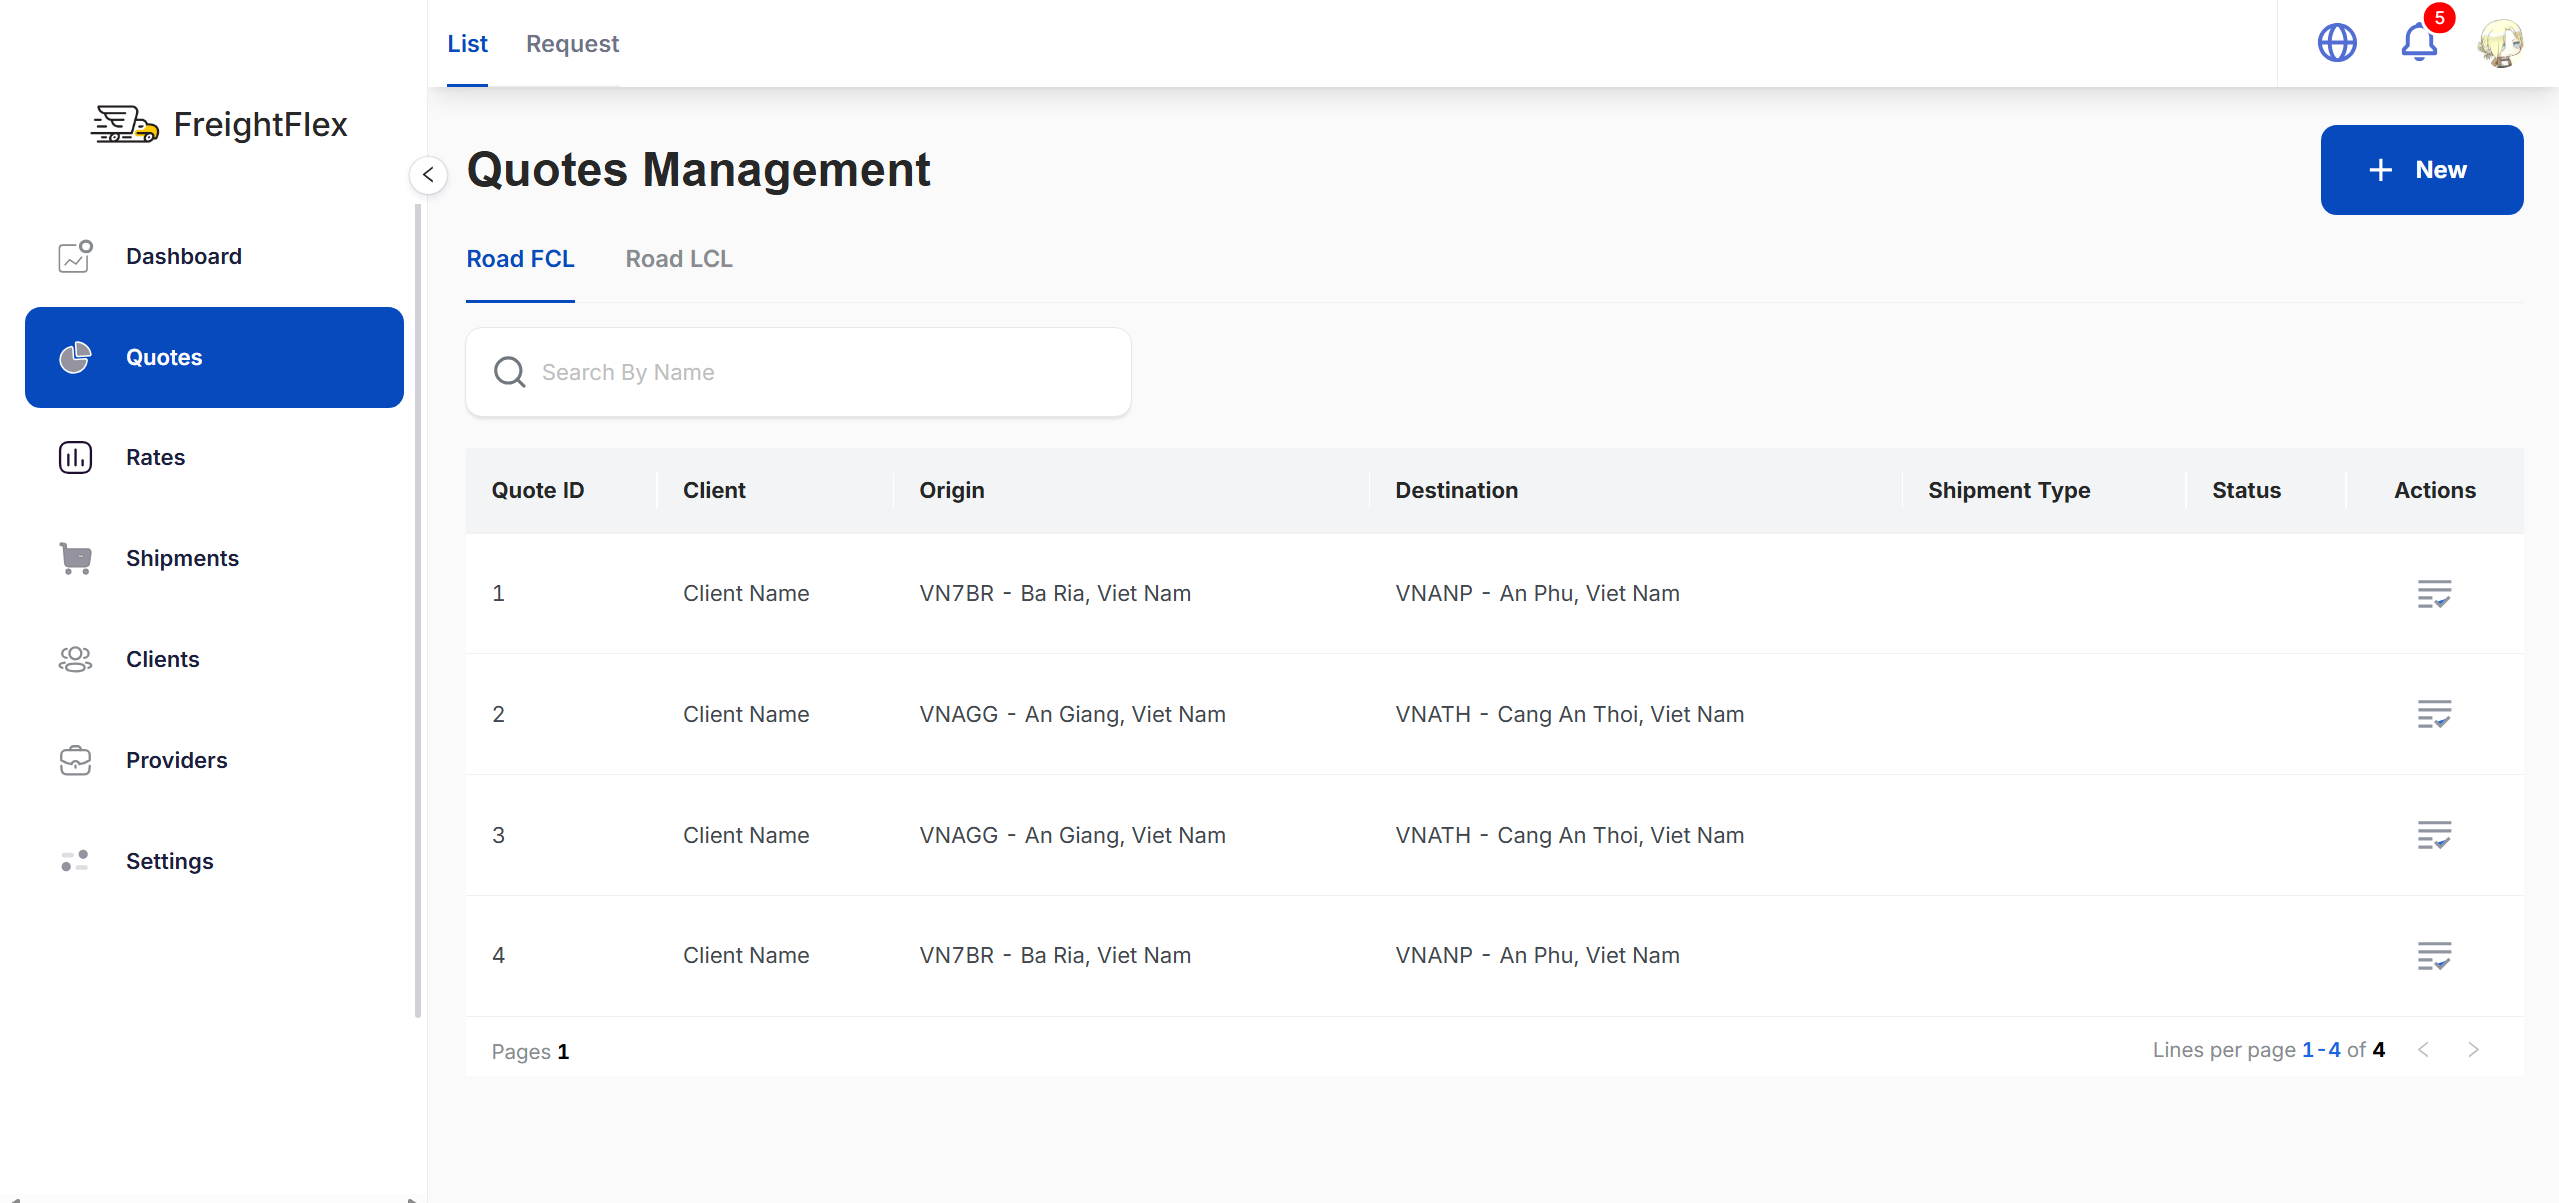
\includegraphics[width=15cm]{graphics/UI/quote-managemet.png}
    \caption{Quote Management}
    \label{fig:quote-management}
\end{figure}

\begin{figure}[H]
    \centering
    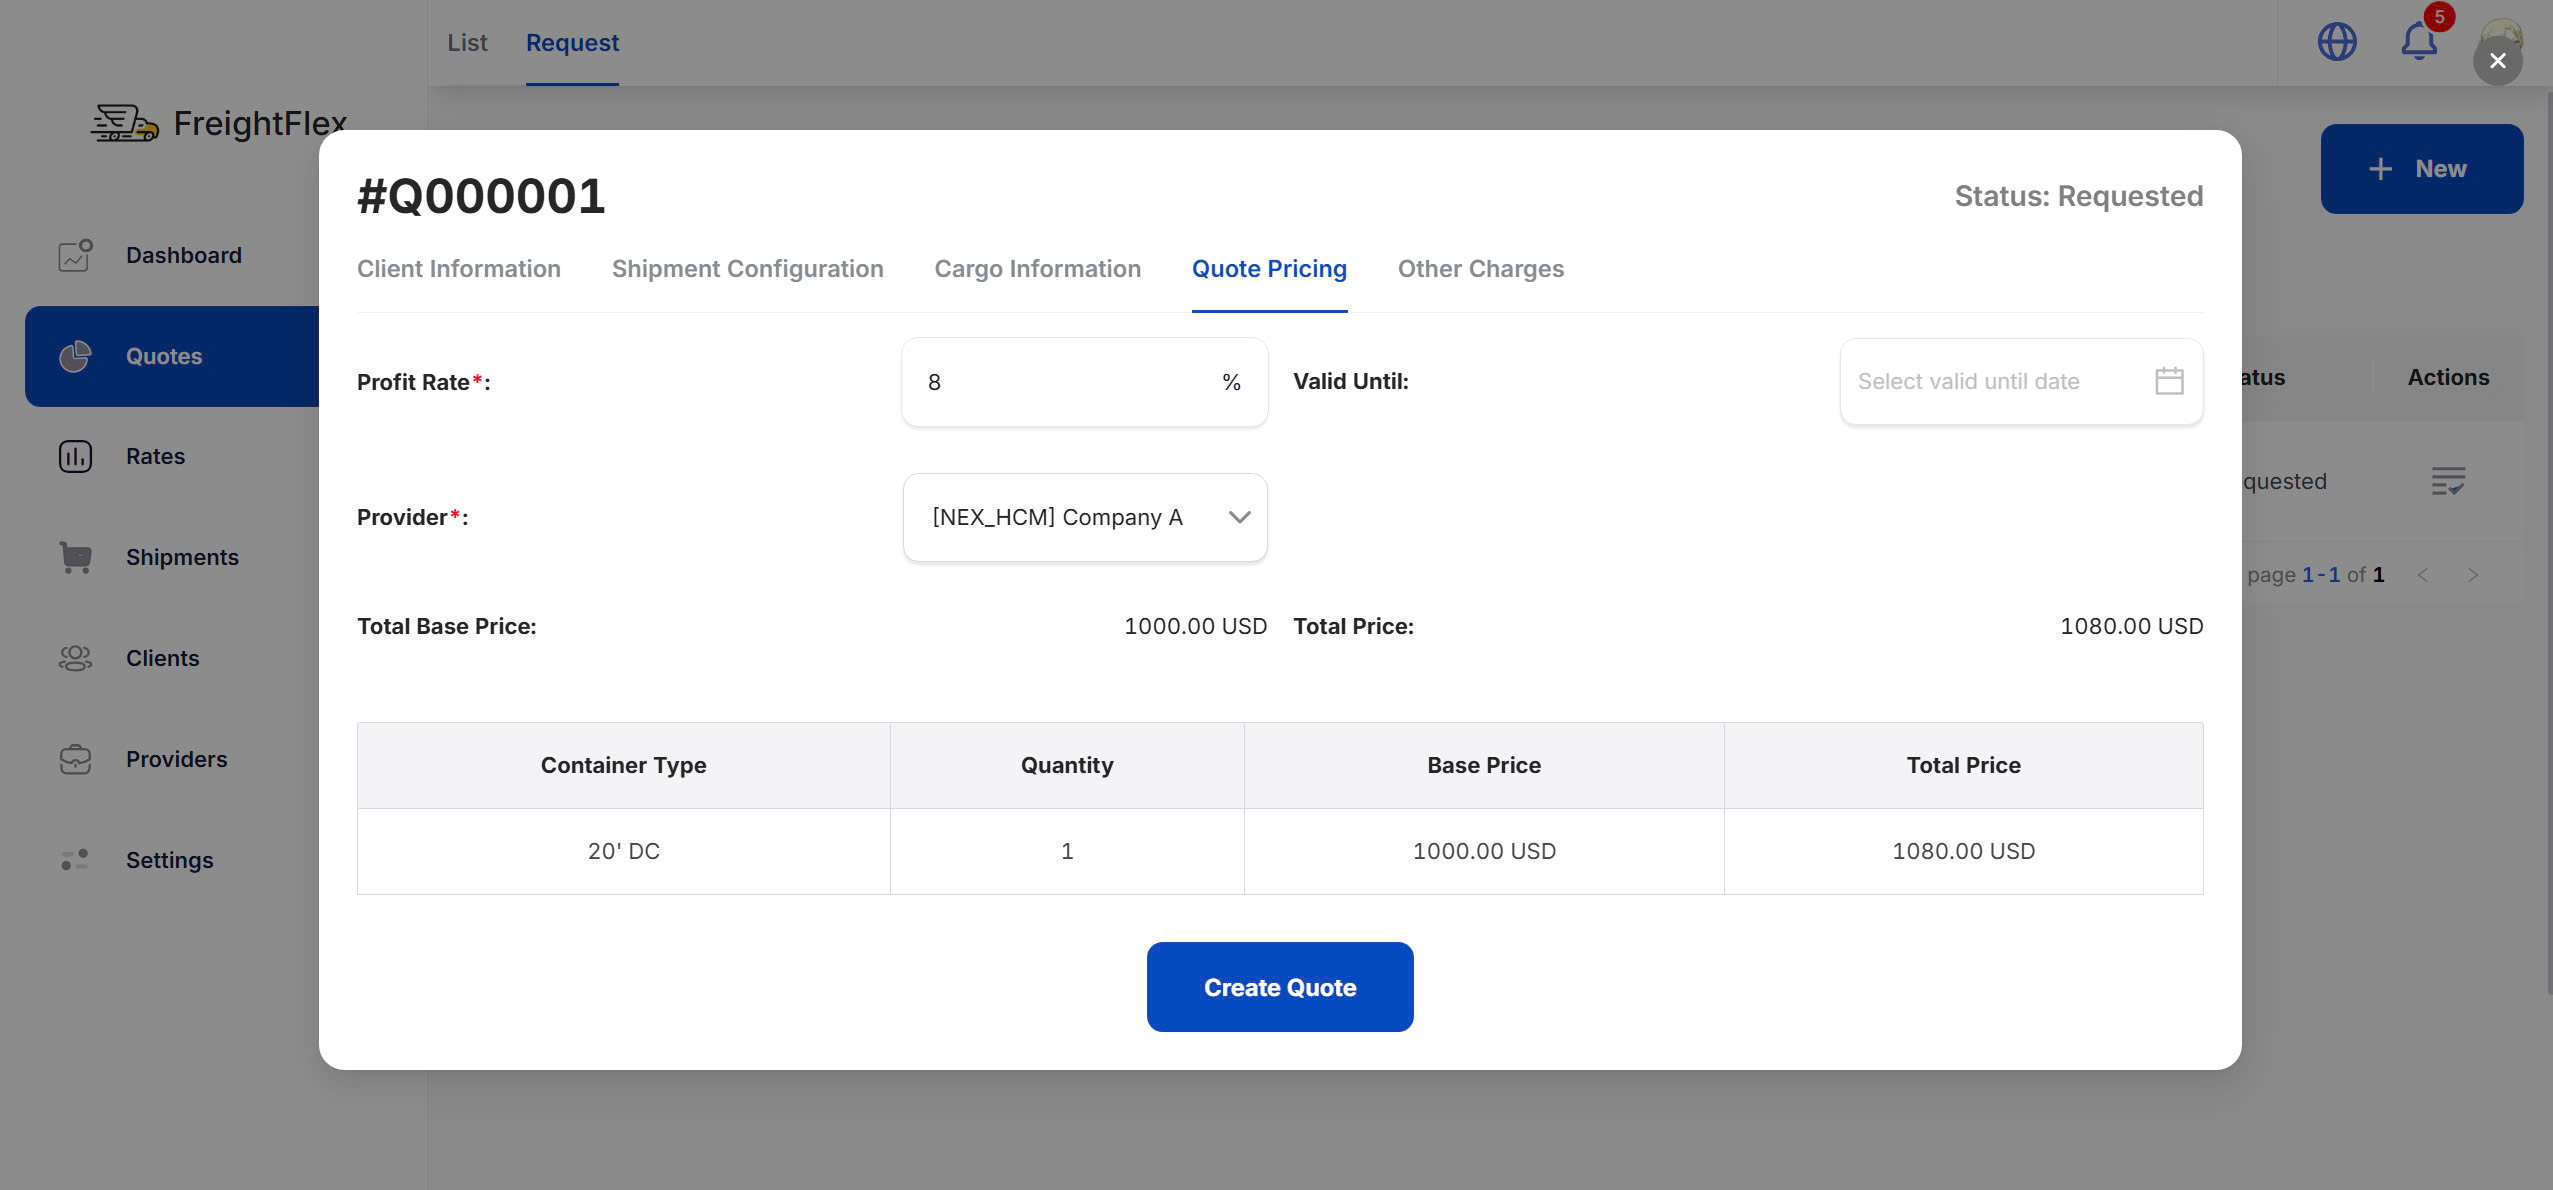
\includegraphics[width=15cm]{graphics/UI/quote-pricing.png}
    \caption{New Quote Creation}
    \label{fig:new-quotes}
\end{figure}

\begin{figure}[H]
    \centering
    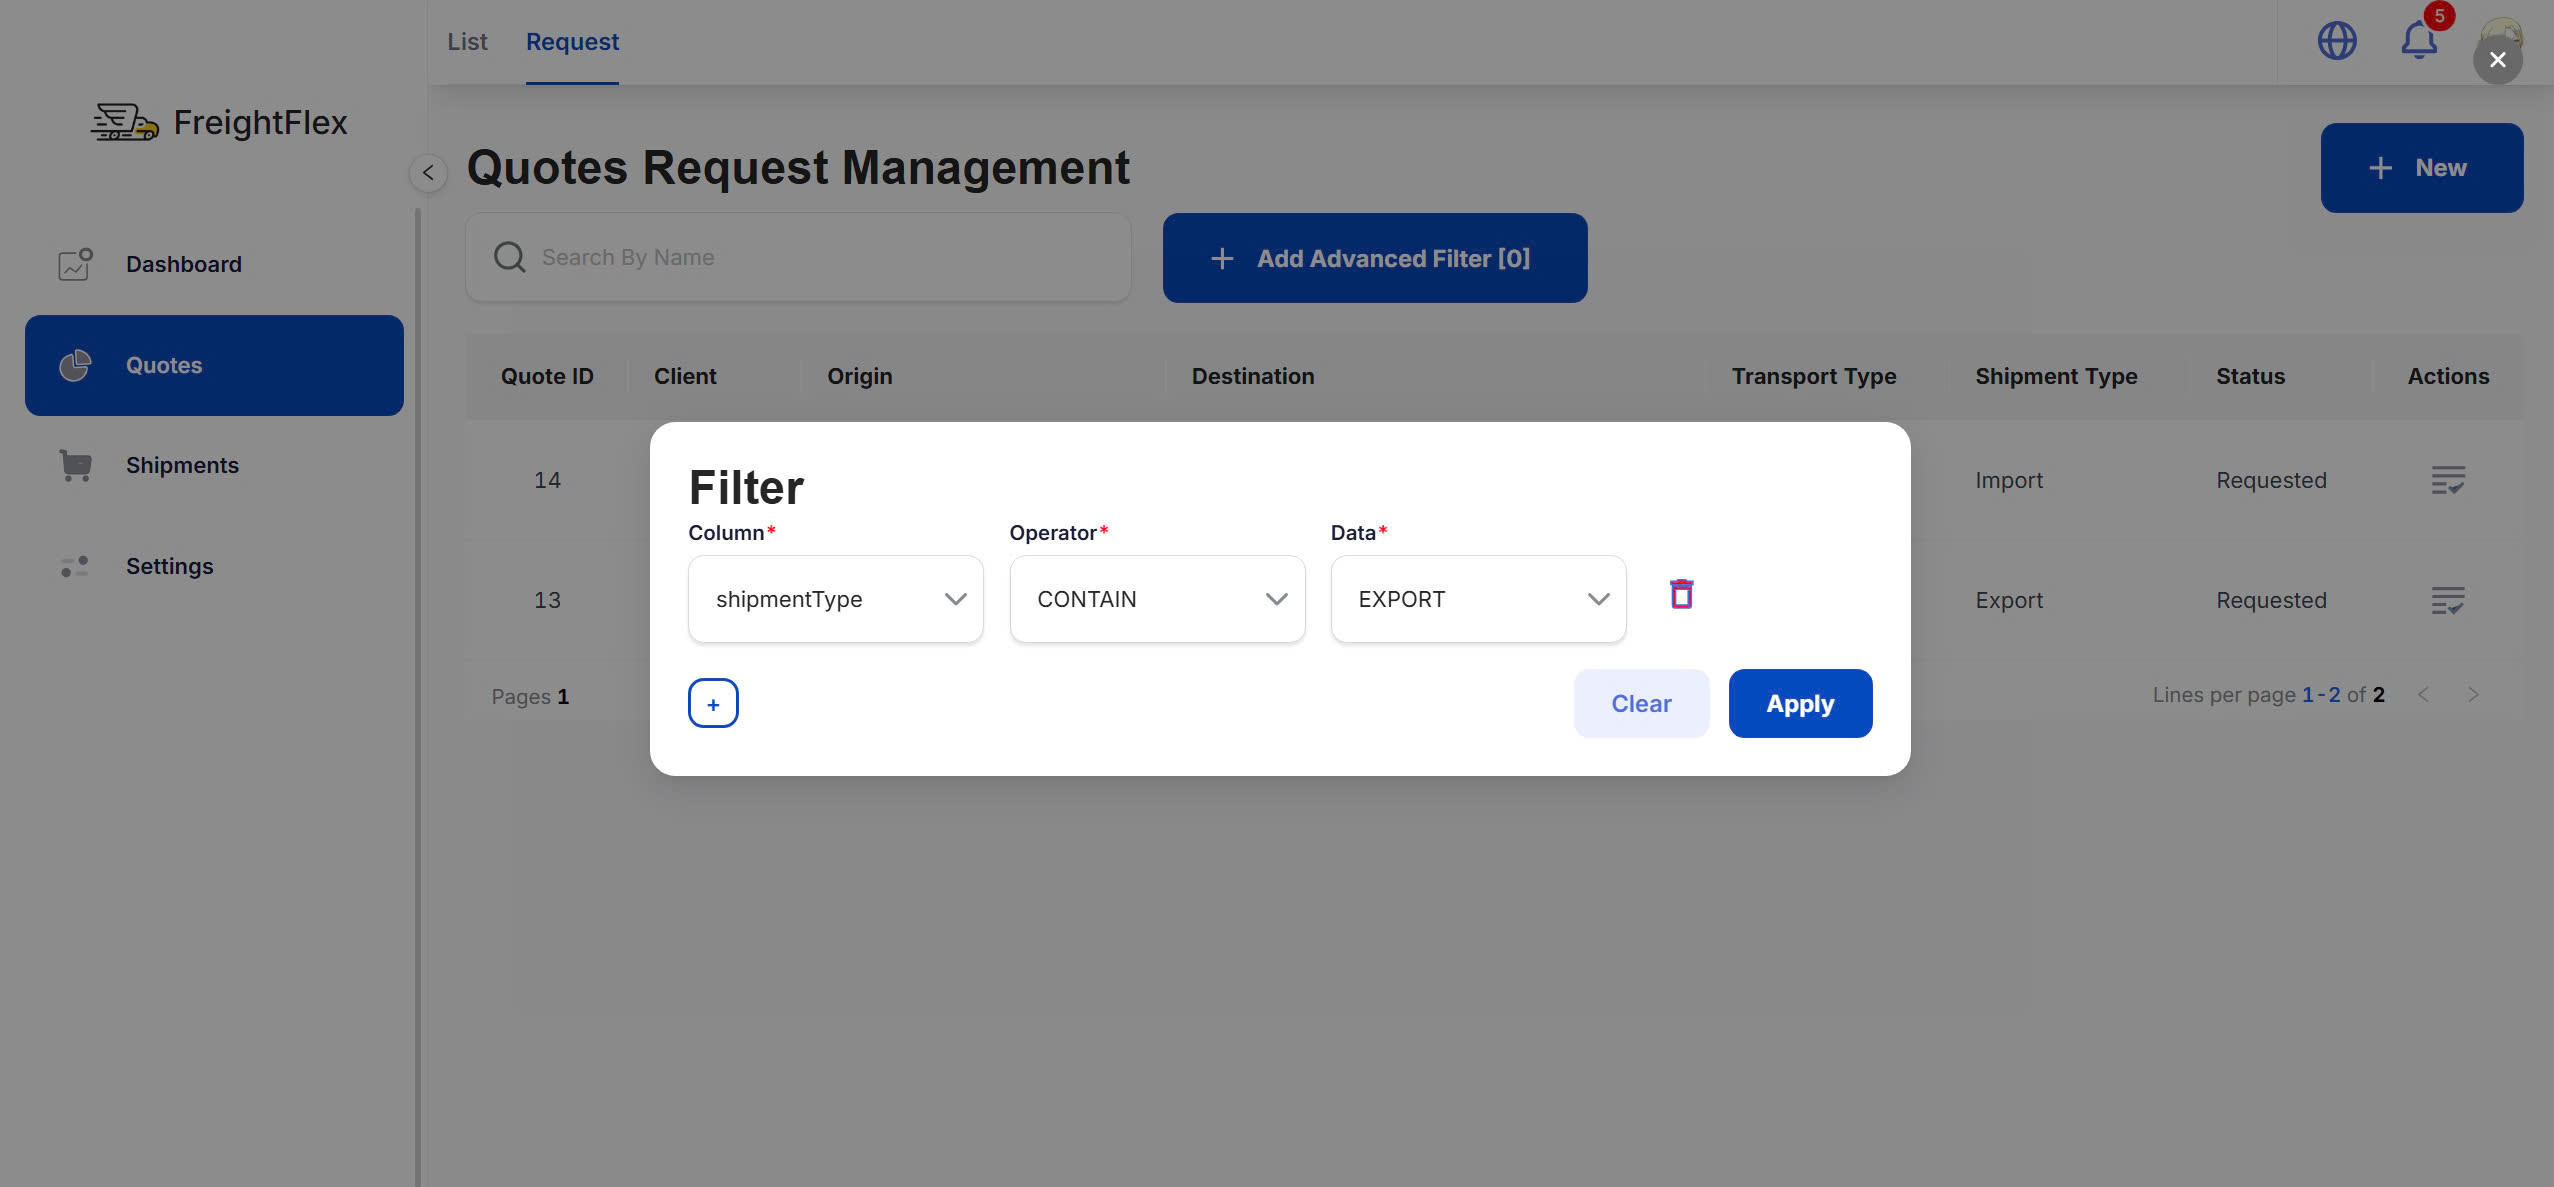
\includegraphics[width=15cm]{graphics/UI/quote-filter.png}
    \caption{Quote Filter}
    \label{fig:new-quotes}
\end{figure}

\section{Third-Party Integrations}
\subsection{File Upload and Storage with Minio}
Minio \cite{minio} is an open-source object storage server that provides a high-performance, S3-compatible API for storing and retrieving unstructured data. We integrated Minio into our system to handle file uploads and storage efficiently. The integration allows users to upload files directly from the frontend, which are then securely stored in Minio's object storage.

Steps to integrate Minio into our system:
\begin{itemize}
    \item \textbf{Infrastructure Setup:} Deployed Minio as a Docker container to provide consistent development and production environments. The Docker configuration ensures easy deployment and maintenance of the storage service.
    
    \item \textbf{Configuration:} Added Minio configuration parameters to our application properties file to establish connectivity between our Spring Boot application and the Minio server:
    
    \begin{verbatim}
minio:
  endpoint: http://localhost:9000
  accessKey: minioadmin
  secretKey: minioadmin
  bucketName: files
    \end{verbatim}
    
    \item \textbf{Dependency Integration:} Added the Minio Java client dependency to our project's pom.xml file:
    
    \begin{verbatim}
<dependency>
    <groupId>io.minio</groupId>
    <artifactId>minio</artifactId>
    <version>8.5.2</version>
</dependency>
    \end{verbatim}
    
    \item \textbf{Service Layer Development:} Created a service class to encapsulate all interactions with the Minio server, including file uploads, downloads, and pre-signed URL generation.
    
    \item \textbf{Entity Creation:} Designed a Document entity to store metadata about files uploaded to Minio:
    
    \begin{verbatim}
@Entity
@Table(name = "document")
public class Document {
    @Id
    private Long id;
    private String name;     // Original file name
    private String type;     // File MIME type
    private String path;     // Path in Minio storage
    private String description;
    private LocalDateTime createdAt;
    private Long createdBy;
}
    \end{verbatim}
    
    \item \textbf{Controller Implementation:} Developed REST endpoints to handle file operations, including upload, download, and deletion.
    
    \item \textbf{Security Integration:} Implemented secure file access controls using pre-signed URLs, allowing temporary access to files without exposing storage credentials.
    
    \item \textbf{Unique File Naming:} Created a strategy to ensure unique file names by generating timestamps or UUIDs as prefixes for all uploaded files.
    
    \item \textbf{Frontend Component Development:} Built frontend components to facilitate file uploads and display stored files to users.
\end{itemize}

The integration provides several key benefits to our system:

\begin{itemize}
    \item \textbf{Scalability:} Minio's object storage architecture allows for horizontal scaling to handle increasing storage demands.
    
    \item \textbf{Cost-Effectiveness:} By using an open-source solution, we avoided vendor lock-in and associated costs of commercial storage services.
    
    \item \textbf{Performance:} Direct uploads to Minio reduce the load on our application servers and provide faster file operations.
    
    \item \textbf{Security:} The separation of file storage from application logic enhances overall system security.
    
    \item \textbf{Compatibility:} The S3-compatible API ensures our application can transition to other storage solutions if needed in the future.
\end{itemize}